%% ============================================================================
%%  CAPITOLO 8 — Integrali definiti
%%  Fonte principale per argomenti e dimostrazioni: Marcellini–Sbordone, cap. 8
%%  (§61 il metodo di esaustione; §62 definizioni e notazioni; §63 proprietà
%%  degli integrali definiti; §64 il teorema della media; appendice: §65
%%  uniforme continuità, teorema di Cantor, funzioni lipschitziane; §66
%%  integrabilità delle funzioni continue).
%% ============================================================================
\aperturacapitolo{Integrali definiti}{cap:integrali-definiti}

\epigraph{Also zuerst: Was hat man unter $\int_{a}^{b}f(x)\,dx$ zu verstehen?\\[2pt]
\upshape(Dunque, per prima cosa: che cosa si deve intendere con
$\int_{a}^{b}f(x)\,dx$?)}{Bernhard Riemann, \emph{Über die Darstellbarkeit einer
Function durch eine trigonometrische Reihe} (1854), \S4}

\lettrine[lines=3, findent=2pt, nindent=0pt]{S}{e la derivata} risponde alla domanda
«quanto rapidamente varia una grandezza?», l'integrale risponde alla domanda inversa:
«quanto si accumula una grandezza che varia?». Lo spazio percorso da un velivolo durante
la corsa di decollo è l'accumulo della sua velocità nel tempo; la portanza totale di
un'ala è l'accumulo della portanza delle singole «strisce» lungo l'apertura; la
superficie alare è l'accumulo delle corde. In tutti questi casi la grandezza da
accumulare non è costante, e il prodotto «base per altezza», che basterebbe se lo
fosse, va sostituito da un procedimento più raffinato.

Il procedimento risale ad Archimede: si suddivide l'intervallo in tanti piccoli
intervalli, in ciascuno dei quali la grandezza è \emph{quasi} costante, e si sommano i
contributi. Si ottengono così due stime, una per difetto e una per eccesso, tanto più
vicine quanto più fine è la suddivisione. L'integrale definito è il numero, se esiste ed
è unico, che separa tutte le stime per difetto da tutte le stime per eccesso: una
definizione che poggia direttamente sull'assioma di completezza del
\cref{cap:numeri}. Studieremo le proprietà dell'integrale (additività, linearità,
confronto), il teorema della media e, in appendice, il risultato che rende la teoria
davvero utilizzabile: \emph{ogni funzione continua in un intervallo chiuso e limitato è
integrabile}. Per dimostrarlo introdurremo la nozione di \emph{uniforme continuità}.
Il calcolo effettivo degli integrali, attraverso il legame con le derivate scoperto da
Newton e Leibniz, sarà l'argomento del prossimo capitolo; qui ne vedremo soltanto un
primo, sorprendente indizio. Seguiremo il testo di riferimento
\cite{marcellini-sbordone}, con qualche integrazione da \cite{giusti}.

\medskip
\noindent\textbf{In questo capitolo.}
\begin{itemize}
  \item Il metodo di esaustione: l'area del settore di parabola
  (\S\ref{sec:esaustione}).
  \item Approfondimento: la quadratura della parabola di Archimede
  (\S\ref{subsec:archimede-parabola}).
  \item Partizioni, somme integrali, integrale definito secondo Riemann; il criterio
  di integrabilità (\S\ref{sec:integrale-definito}).
  \item Approfondimento: l'integrale con le funzioni a scala
  (\S\ref{subsec:funzioni-scala}).
  \item Proprietà: additività, linearità, confronto, valore assoluto; l'area con segno
  (\S\ref{sec:proprieta-integrale}).
  \item Il teorema della media; corda media e corda media aerodinamica di un'ala
  (\S\ref{sec:media}).
  \item Appendice: uniforme continuità, teorema di Cantor, funzioni lipschitziane
  (\S\ref{sec:uniforme-continuita}).
  \item Appendice: integrabilità delle funzioni continue e delle funzioni monotòne;
  le somme di Riemann e le formule di quadratura (\S\ref{sec:integrabilita-continue}).
  \item Esercizi di riepilogo (\S\ref{sec:esercizi-cap8}).
  \item Punti fondamentali del capitolo (\S\ref{sec:sintesi-cap08}).
\end{itemize}

%% ----------------------------------------------------------------------------
%%  §8.1  Il metodo di esaustione
%% ----------------------------------------------------------------------------
\section{Il metodo di esaustione}
\label{sec:esaustione}

Con l'espressione \emph{metodo di esaustione}\index{metodo di esaustione} si indica il
procedimento con cui i matematici greci calcolavano aree e volumi di figure
curvilinee. Lo usò sistematicamente Archimede nel \textsc{iii} secolo a.C., ma, secondo
lo stesso Archimede, risale a Eudosso di Cnido (\textsc{iv} secolo a.C.). Ne abbiamo già
visto un esempio nel \cref{sec:premessa-limiti}: l'area del cerchio è stata ottenuta
come limite delle aree dei poligoni regolari inscritti, e nel \cref{teo:area-cerchio}
abbiamo dimostrato che tale limite è $\pi$. La parola «esaustione» esprime proprio
l'idea che il cerchio viene \emph{riempito}, o \emph{esaurito}, da poligoni con un
numero di lati sempre maggiore.

In questo paragrafo descriviamo il metodo con il linguaggio moderno dei limiti, su un
esempio che guiderà la definizione generale del paragrafo successivo: l'area del
\emph{settore di parabola}, cioè della regione
\begin{equation}\label{eq:settore-parabola}
  S=\set{(x,y)\in\R^{2} \tc 0\le x\le b,\ \ 0\le y\le x^{2}}, \qquad b>0,
\end{equation}
compresa tra l'asse delle $x$, il grafico di $f(x)=x^{2}$ e la retta verticale $x=b$
(\cref{fig:esaustione}, a sinistra).

\subsection{Stime per difetto e per eccesso}

Dividiamo l'intervallo $[0,b]$ in $n\in\N$ intervalli $[x_{k-1},x_{k}]$ di uguale
ampiezza $b/n$, mediante i punti
\begin{equation}\label{eq:partizione-uniforme-parabola}
  x_{0}=0,\quad x_{1}=\frac bn,\quad x_{2}=\frac{2b}n,\quad\dots,\quad
  x_{k}=\frac{kb}n,\quad\dots,\quad x_{n}=b .
\end{equation}
Poiché $f(x)=x^{2}$ è crescente in $[0,b]$, in ciascun intervallo $[x_{k-1},x_{k}]$ si
ha $x_{k-1}^{2}\le x^{2}\le x_{k}^{2}$. Il rettangolo di base $[x_{k-1},x_{k}]$ e altezza
$x_{k-1}^{2}$ è dunque contenuto in $S$, mentre quello di uguale base e altezza
$x_{k}^{2}$ contiene la parte di $S$ che sta sopra $[x_{k-1},x_{k}]$
(\cref{fig:esaustione}, al centro e a destra). Sommando le aree dei rettangoli
otteniamo
\begin{align}
  s_{n}&=\sum_{k=1}^{n}f(x_{k-1})(x_{k}-x_{k-1})=\frac bn\sum_{k=1}^{n}x_{k-1}^{2}
  =\frac bn\bigl(x_{0}^{2}+x_{1}^{2}+\dots+x_{n-1}^{2}\bigr),
  \label{eq:somma-inferiore-parabola}\\
  S_{n}&=\sum_{k=1}^{n}f(x_{k})(x_{k}-x_{k-1})=\frac bn\sum_{k=1}^{n}x_{k}^{2}
  =\frac bn\bigl(x_{1}^{2}+x_{2}^{2}+\dots+x_{n}^{2}\bigr).
  \label{eq:somma-superiore-parabola}
\end{align}
La prima è l'area di un'unione di rettangoli (un \emph{plurirettangolo}) contenuta in
$S$, la seconda quella di un plurirettangolo che contiene $S$. Se attribuiamo all'area
le proprietà che l'intuizione suggerisce (l'area di un rettangolo è base per altezza,
l'area di un'unione di figure senza punti interni comuni è la somma delle aree, una
figura contenuta in un'altra ha area minore o uguale), otteniamo
\begin{equation}\label{eq:stime-parabola}
  s_{n}\le\text{area }S\le S_{n} \qquad\perogni n\in\N .
\end{equation}
La somma $s_{n}$ è detta \emph{somma integrale inferiore}, la somma $S_{n}$
\emph{somma integrale superiore}.

\begin{figure}[htb]
\centering
\begin{tikzpicture}
\begin{axis}[name=p1, width=0.38\textwidth, height=0.36\textwidth,
  axis lines=left, xmin=0, xmax=1.15, ymin=0, ymax=1.15, xtick={1},
  xticklabels={$b$}, ytick={1}, yticklabels={$b^{2}$},
  title={\scriptsize il settore $S$}, clip=false]
  \addplot[draw=none, fill=blu!18, domain=0:1, samples=60] {x^2} \closedcycle;
  \addplot[curva, domain=0:1.08, samples=60] {x^2};
  \addplot[tratteggio] coordinates {(1,0) (1,1)};
  \node[font=\scriptsize, blu] at (axis cs:0.72,0.2) {$S$};
  \node[font=\scriptsize, anchor=east] at (axis cs:0.95,0.95) {$y=x^{2}$};
\end{axis}
\begin{axis}[at={(p1.east)}, anchor=west, xshift=0.5cm, name=p2,
  width=0.38\textwidth, height=0.36\textwidth, axis lines=left, xmin=0, xmax=1.15,
  ymin=0, ymax=1.15, xtick={0,0.1667,0.3333,0.5,0.6667,0.8333,1},
  xticklabels={,,,,,,$b$}, ytick=\empty, title={\scriptsize $s_{6}$ (per difetto)}]
  \addplot[ybar interval, fill=blu!25, draw=blu, domain=0:1, samples=7] {x^2};
  \addplot[curva2, domain=0:1.08, samples=60] {x^2};
\end{axis}
\begin{axis}[at={(p2.east)}, anchor=west, xshift=0.5cm, width=0.38\textwidth,
  height=0.36\textwidth, axis lines=left, xmin=0, xmax=1.15, ymin=0, ymax=1.15,
  xtick={0,0.1667,0.3333,0.5,0.6667,0.8333,1}, xticklabels={,,,,,,$b$},
  ytick=\empty, title={\scriptsize $S_{6}$ (per eccesso)}]
  \addplot[ybar interval, fill=rame!25, draw=rame, domain=0:1, samples=7]
    {(x+1/6)^2};
  \addplot[curva, domain=0:1.08, samples=60] {x^2};
\end{axis}
\end{tikzpicture}
\caption{Il settore di parabola $S$ (a sinistra) e le sue approssimazioni con $n=6$
rettangoli: per difetto, con altezze $x_{k-1}^{2}$ (al centro), e per eccesso, con
altezze $x_{k}^{2}$ (a destra).}
\label{fig:esaustione}
\end{figure}

Calcoliamo le due somme. Ricordando che $x_{k}=kb/n$ e usando la formula della somma
dei primi $n$ quadrati, dimostrata per induzione nella \cref{prop:quadrati},
\[
  \sum_{k=1}^{n}x_{k}^{2}=\frac{b^{2}}{n^{2}}\sum_{k=1}^{n}k^{2}
  =\frac{b^{2}}{n^{2}}\cdot\frac{n(n+1)(2n+1)}6 ,
\]
e quindi $S_{n}=\frac bn\sum x_{k}^{2}$ vale
\begin{equation}\label{eq:Sn-parabola}
  S_{n}=\frac{b^{3}}6\cdot\frac{(n+1)(2n+1)}{n^{2}} .
\end{equation}
Nella somma inferiore compaiono i quadrati di $x_{0},\dots,x_{n-1}$, cioè la stessa somma
con $n-1$ al posto di $n$ (il termine $x_{0}^{2}=0$ non contribuisce):
\begin{equation}\label{eq:sn-parabola}
  s_{n}=\frac bn\cdot\frac{b^{2}}{n^{2}}\cdot\frac{(n-1)n(2n-1)}6
  =\frac{b^{3}}6\cdot\frac{(n-1)(2n-1)}{n^{2}} .
\end{equation}
Prima di passare al limite osserviamo una semplificazione notevole. La differenza tra
le due somme è una somma \emph{telescopica}, nella quale i termini intermedi si
cancellano a due a due (come nella \cref{prop:telescopica}):
\begin{equation}\label{eq:differenza-parabola}
  S_{n}-s_{n}=\frac bn\sum_{k=1}^{n}\bigl(x_{k}^{2}-x_{k-1}^{2}\bigr)
  =\frac bn\bigl(x_{n}^{2}-x_{0}^{2}\bigr)=\frac{b^{3}}n .
\end{equation}
Il significato geometrico è illuminante: i rettangolini di base $[x_{k-1},x_{k}]$ e
altezza $x_{k}^{2}-x_{k-1}^{2}$, che costituiscono la differenza tra i due
plurirettangoli, traslati orizzontalmente fino all'ultima colonna vi si impilano senza
sovrapporsi,
formando un unico rettangolo di base $b/n$ e altezza $b^{2}$ (\cref{fig:telescopica}).
La differenza tende a zero come $1/n$.

\begin{figure}[htb]
\centering
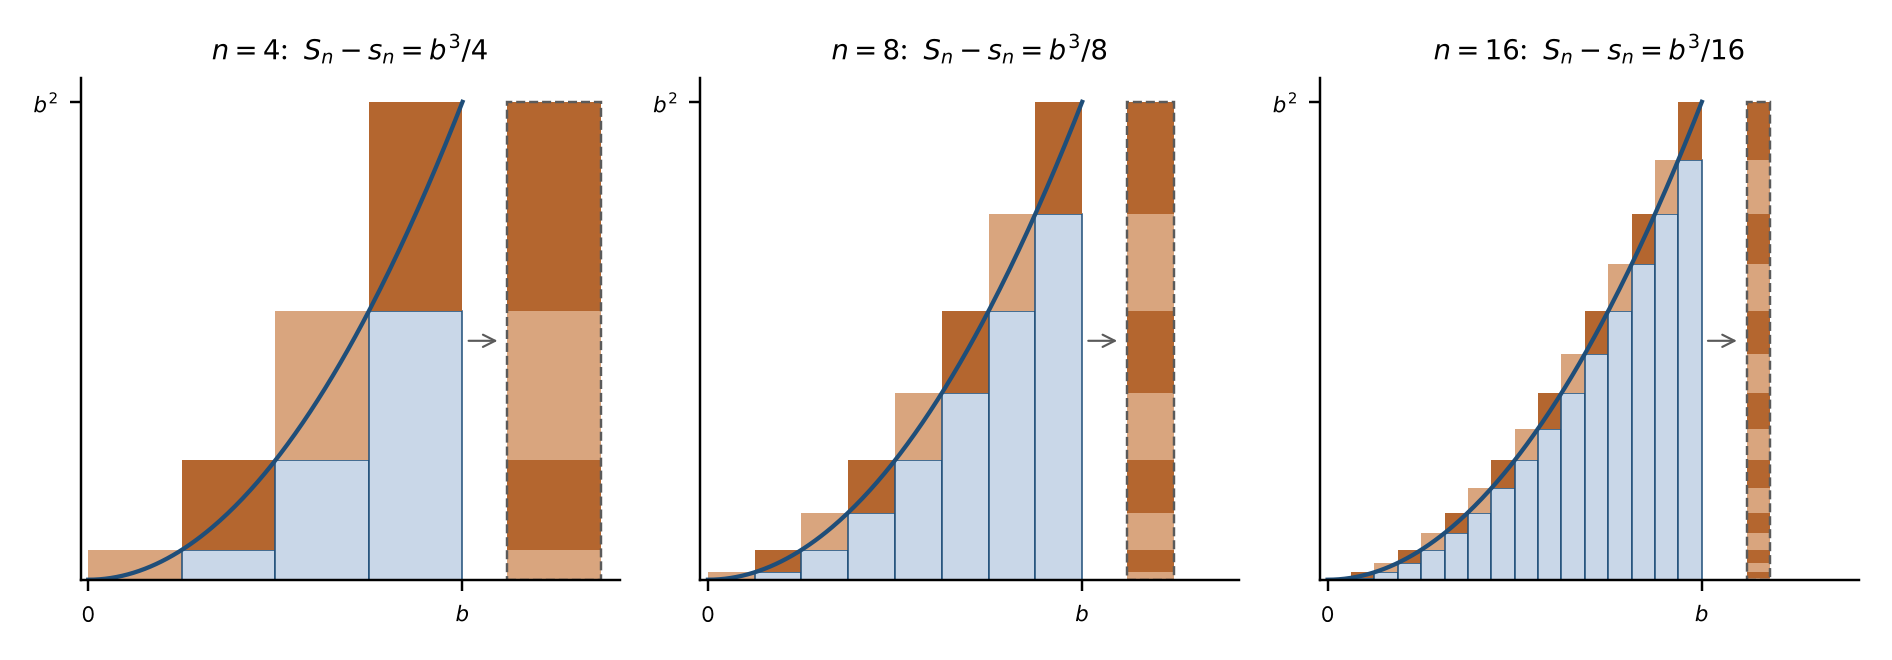
\includegraphics[width=\textwidth]{figure/esaustione.png}
\caption{La differenza $S_{n}-s_{n}=b^{3}/n$ per $n=4,8,16$. I rettangolini in color rame
(la parte di plurirettangolo circoscritto che eccede quello inscritto) si possono
traslare nell'ultima colonna, dove formano il rettangolo tratteggiato di base $b/n$ e
altezza $b^{2}$: la differenza vale esattamente $b^{3}/n$
(\texttt{python/fig\_esaustione.py}).}
\label{fig:telescopica}
\end{figure}

\needspace{12\baselineskip}
\subsection{L'area del settore di parabola}

\begin{proposizione}[Area del settore di parabola]\label{prop:settore-parabola}
Sia $b>0$ e siano $s_{n}$, $S_{n}$ le somme
\eqref{eq:somma-inferiore-parabola}--\eqref{eq:somma-superiore-parabola}. Allora
$b^{3}/3$ è l'\emph{unico} numero reale $c$ tale che
\begin{equation}\label{eq:separatore-parabola}
  s_{n}\le c\le S_{n} \qquad\perogni n\in\N .
\end{equation}
\end{proposizione}

\begin{schema}
\Ipotesi{$b>0$; \ $s_{n}$, $S_{n}$ somme inferiori e superiori di $x^{2}$ in $[0,b]$
relative alla suddivisione in $n$ parti uguali.}
\Tesi{(i) $s_{n}<\frac{b^{3}}3<S_{n}$ per ogni $n$; \ (ii) se $s_{n}\le c\le S_{n}$ per ogni
$n$, allora $c=\frac{b^{3}}3$.}
\end{schema}

\begin{strategia}
Le formule \eqref{eq:Sn-parabola} e \eqref{eq:sn-parabola} sono esplicite: sviluppando i
prodotti, entrambe si scrivono come $\frac{b^{3}}3$ più o meno termini che contengono
$\frac1n$ e $\frac1{n^{2}}$, e un confronto di segni prova la (i). Per l'unicità basta
osservare che due numeri compresi tra $s_{n}$ e $S_{n}$ distano al più
$S_{n}-s_{n}=\frac{b^{3}}n$, quantità che, per la proprietà di Archimede, diventa più
piccola di qualsiasi numero positivo assegnato.
\end{strategia}

\begin{dimostrazione}
(i) Sviluppando i prodotti nelle \eqref{eq:Sn-parabola} e \eqref{eq:sn-parabola},
\[
\begin{aligned}
  S_{n}&=\frac{b^{3}}6\cdot\frac{2n^{2}+3n+1}{n^{2}}
  =\frac{b^{3}}3+\frac{b^{3}}{2n}+\frac{b^{3}}{6n^{2}},\\
  s_{n}&=\frac{b^{3}}6\cdot\frac{2n^{2}-3n+1}{n^{2}}
  =\frac{b^{3}}3-\frac{b^{3}}{6n^{2}}\,(3n-1) .
\end{aligned}
\]
La prima mostra che $S_{n}>\frac{b^{3}}3$; nella seconda $3n-1>0$ per ogni $n\ge1$, e
quindi $s_{n}<\frac{b^{3}}3$.

(ii) Sia $c$ un numero che verifica la \eqref{eq:separatore-parabola}. Poiché anche
$\frac{b^{3}}3$ la verifica, i due numeri appartengono entrambi all'intervallo
$[s_{n},S_{n}]$, e quindi, per la \eqref{eq:differenza-parabola},
\[
  \Bigl|c-\frac{b^{3}}3\Bigr|\le S_{n}-s_{n}=\frac{b^{3}}n \qquad\perogni n\in\N .
\]
Se fosse $c\neq\frac{b^{3}}3$, per la proprietà di Archimede (\cref{teo:archimede})
esisterebbe $n\in\N$ con $n\,\bigl|c-\frac{b^{3}}3\bigr|>b^{3}$, contro la disuguaglianza
appena scritta. Dunque $c=\frac{b^{3}}3$.
\end{dimostrazione}

Dalle \eqref{eq:stime-parabola} e dalla proposizione segue che, se il settore $S$ ha
un'area, essa non può che essere
\begin{equation}\label{eq:area-parabola}
  \text{area }S=\frac{b^{3}}3 ,
\end{equation}
cioè \emph{un terzo} dell'area del rettangolo $[0,b]\times[0,b^{2}]$ che lo contiene.
È il risultato di Archimede. Allo stesso valore si arriva passando al limite nelle
\eqref{eq:Sn-parabola}--\eqref{eq:sn-parabola} (basta dividere numeratore e denominatore
per $n^{2}$): $s_{n}\to\frac{b^{3}}3$ e $S_{n}\to\frac{b^{3}}3$. Le due strade sono
equivalenti, ma la prima, che caratterizza l'area come \emph{unico elemento separatore}
tra le stime per difetto e quelle per eccesso, è quella che generalizzeremo.

Il programma seguente calcola le somme in aritmetica razionale esatta, con il modulo
\texttt{fractions}, per $b=1$: si vede la differenza $S_{n}-s_{n}=\frac1n$ e
l'avvicinamento di entrambe le somme a $\frac13$.

\begin{python}[Somme integrali del settore di parabola in aritmetica esatta]
from fractions import Fraction as F

def somme(n, b=F(1)):
    """Somme inferiore e superiore di x^2 in [0, b], n intervalli."""
    x = [F(k, n) * b for k in range(n + 1)]
    s = sum(x[k - 1]**2 * (x[k] - x[k - 1]) for k in range(1, n + 1))
    S = sum(x[k]**2 * (x[k] - x[k - 1]) for k in range(1, n + 1))
    return s, S

print(f"{'n':>5} {'s_n':>10} {'S_n':>10} {'S_n - s_n':>10}")
for n in (1, 2, 5, 10, 100, 1000):
    s, S = somme(n)
    print(f"{n:5d} {float(s):10.6f} {float(S):10.6f}"
          f" {float(S - s):10.6f}")
s, S = somme(10)
print("n = 10, valori esatti:", s, "< 1/3 <", S)
\end{python}
\begin{risultato}
    n        s_n        S_n  S_n - s_n
    1   0.000000   1.000000   1.000000
    2   0.125000   0.625000   0.500000
    5   0.240000   0.440000   0.200000
   10   0.285000   0.385000   0.100000
  100   0.328350   0.338350   0.010000
 1000   0.332834   0.333834   0.001000
n = 10, valori esatti: 57/200 < 1/3 < 77/200
\end{risultato}

\begin{osservazione}[Un indizio del teorema fondamentale]\label{oss:indizio-tfc}
Pensiamo l'area \eqref{eq:area-parabola} come funzione dell'estremo $b$ e deriviamola:
\begin{equation}\label{eq:derivata-area}
  \frac{d}{db}\Bigl(\frac{b^{3}}3\Bigr)=b^{2} .
\end{equation}
La derivata dell'area è il valore in $x=b$ della funzione $f(x)=x^{2}$ che delimita la
regione. Non è una coincidenza: se si sposta l'estremo da $b$ a $b+h$, l'area aumenta
di una striscia di base $h$ e altezza circa $b^{2}$, e il rapporto incrementale è
circa $b^{2}$. Questa osservazione, resa rigorosa, è il \emph{teorema fondamentale del
calcolo integrale}, che dimostreremo nel prossimo capitolo e che trasformerà il
calcolo delle aree in un problema di derivate.
\end{osservazione}

\begin{idea}[La teoria delle strisce e la portanza di un'ala]
Lungo l'apertura alare la portanza non è distribuita uniformemente: si descrive con la
\emph{portanza per unità di apertura} $l(y)$, misurata in N/m, dove $y\in[-\frac b2,
\frac b2]$ è la coordinata lungo l'apertura $b$. La portanza totale è l'«area» sotto il
grafico di $l$: per calcolarla, la \emph{teoria delle strisce} divide l'ala in strisce
di larghezza $\Delta y$ e somma i contributi $l(y_{k})\,\Delta y$, esattamente come
abbiamo fatto per la parabola. Un caso fondamentale è la \emph{distribuzione
ellittica}
\begin{equation}\label{eq:portanza-ellittica}
  l(y)=l_{0}\sqrt{1-\Bigl(\frac{2y}b\Bigr)^{2}}, \qquad -\frac b2\le y\le\frac b2,
\end{equation}
che, secondo la teoria della linea portante di Ludwig Prandtl (1918), rende minima la
resistenza indotta a parità di portanza e di apertura; la si ottiene, ad esempio, con
un'ala di pianta ellittica come quella dello Spitfire (\cref{fig:portanza-ellittica}).
Poiché $l$ è crescente in $[-\frac b2,0]$ e decrescente in $[0,\frac b2]$, se lo zero è
un estremo delle strisce, in ogni striscia il minimo e il massimo di $l$ sono assunti
negli estremi della striscia, e le somme per difetto e per eccesso si calcolano
facilmente. Vedremo nell'\cref{es:portanza-ellittica-esatta} che l'area sotto la
\eqref{eq:portanza-ellittica} vale $\frac\pi4l_{0}b$; per un velivolo di peso
$W=10\,000$~N e apertura $b=10$~m, il volo livellato ($L=W$) richiede dunque
$l_{0}=\frac{4W}{\pi b}\approx1273$~N/m.
\end{idea}

\begin{python}[Portanza totale con la teoria delle strisce]
import math

b, W = 10.0, 10000.0                  # apertura [m], peso [N]
l0 = 4 * W / (math.pi * b)            # carico al centro [N/m]

def l(y):
    """Portanza per unità di apertura, distribuzione ellittica."""
    return l0 * math.sqrt(max(0.0, 1 - (2 * y / b)**2))

def strisce(n):
    """Somme per difetto e per eccesso con n strisce (n pari)."""
    y = [-b / 2 + k * b / n for k in range(n + 1)]
    s = S = 0.0
    for k in range(1, n + 1):
        lo, hi = sorted((l(y[k - 1]), l(y[k])))  # l monotona
        s += lo * (y[k] - y[k - 1])
        S += hi * (y[k] - y[k - 1])
    return s, S

print(f"l0 = {l0:.2f} N/m")
for n in (4, 16, 64, 256, 1024):
    s, S = strisce(n)
    print(f"n = {n:4d}: {s:8.1f} N <= L <= {S:8.1f} N"
          f"   (S - s = {S - s:6.1f} N)")
\end{python}
\begin{risultato}
l0 = 1273.24 N/m
n =    4:   5513.3 N <= L <=  11879.5 N   (S - s = 6366.2 N)
n =   16:   9039.4 N <= L <=  10631.0 N   (S - s = 1591.5 N)
n =   64:   9780.4 N <= L <=  10178.3 N   (S - s =  397.9 N)
n =  256:   9947.7 N <= L <=  10047.2 N   (S - s =   99.5 N)
n = 1024:   9987.2 N <= L <=  10012.1 N   (S - s =   24.9 N)
\end{risultato}

\begin{figure}[htb]
\centering
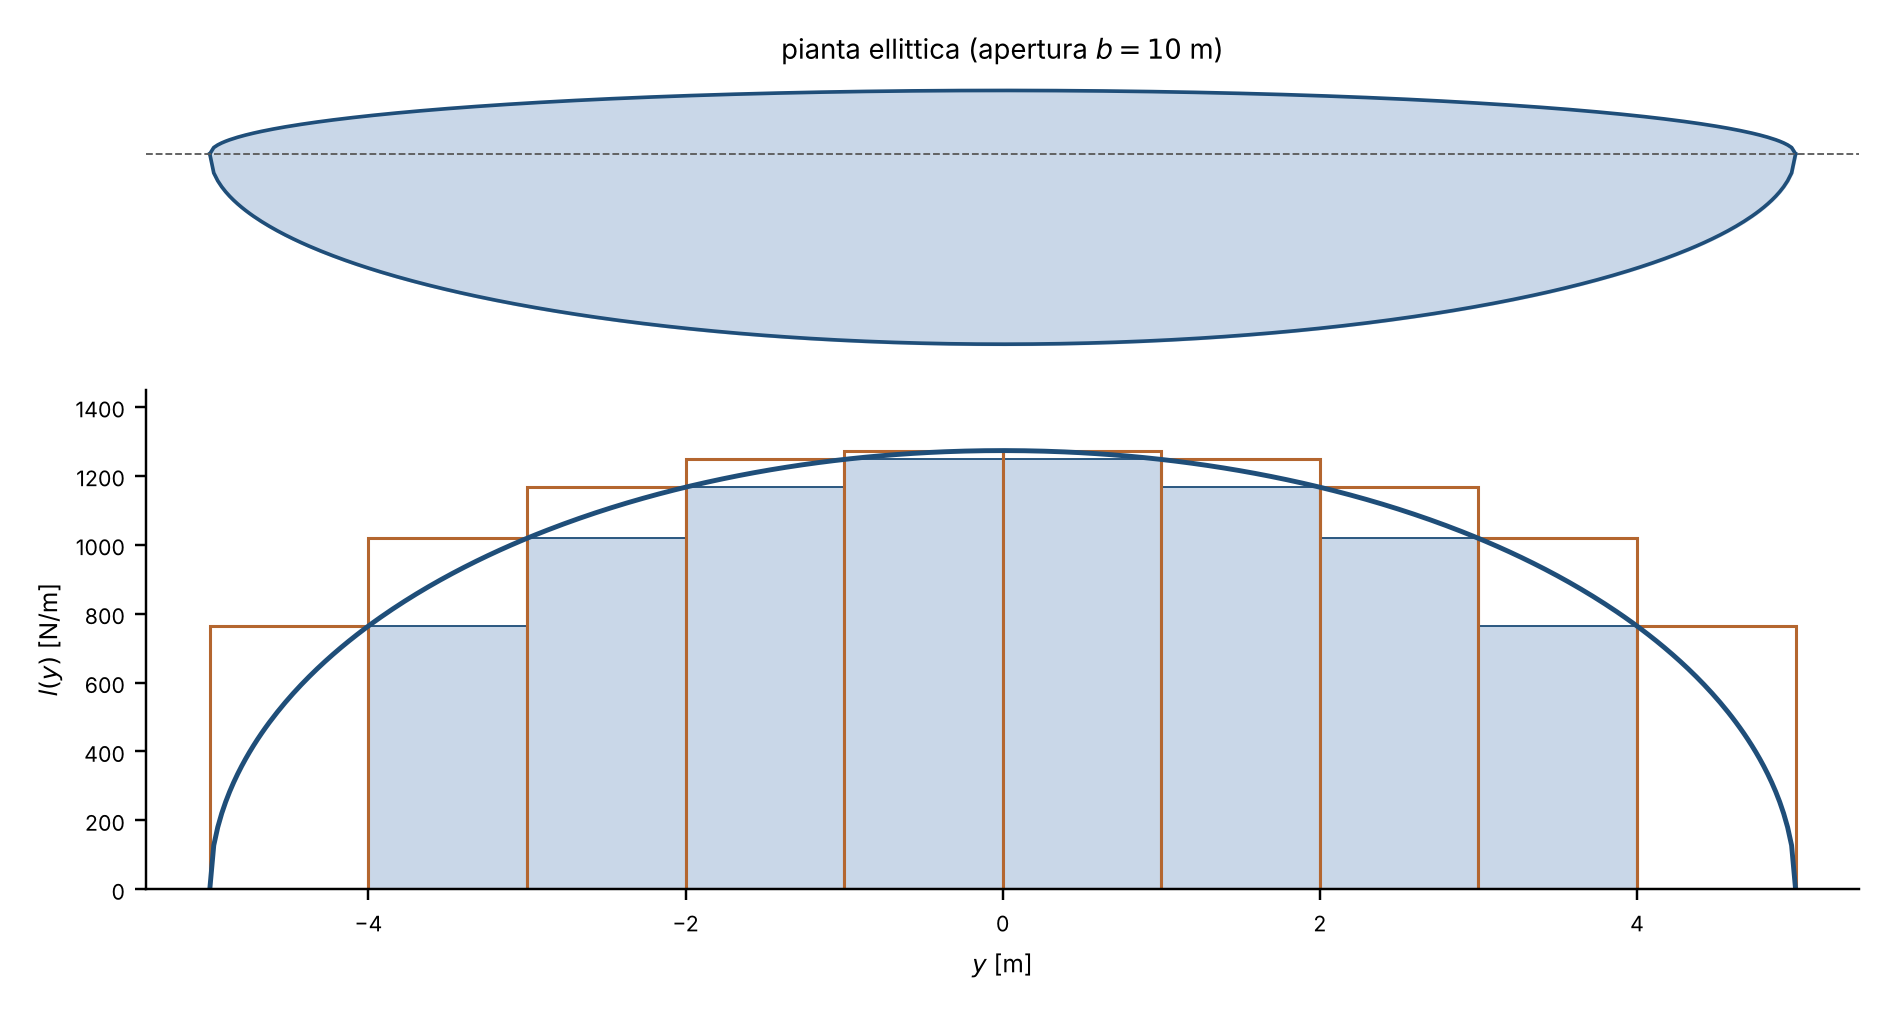
\includegraphics[width=\textwidth]{figure/portanza_ellittica.png}
\caption{In alto, la pianta ellittica di un'ala di apertura $b=10$~m. In basso, la
distribuzione ellittica della portanza \eqref{eq:portanza-ellittica} con $10$ strisce:
in azzurro i rettangoli della somma per difetto, in color rame il contorno di quelli
della somma per eccesso (\texttt{python/fig\_portanza\_ellittica.py}).}
\label{fig:portanza-ellittica}
\end{figure}

Anche qui la differenza tra le due somme è telescopica: in ciascuna delle due metà
dell'ala, dove $l$ è monotòna e passa dal valore $0$ al valore $l_{0}$, essa vale
$\frac{l_{0}b}n$, e in totale $S-s=\frac{2l_{0}b}n$. Le somme convergono al valore
esatto $10\,000$~N, ma lentamente, come $1/n$: nel \cref{sec:integrabilita-continue}
vedremo formule di approssimazione molto più efficienti.

\begin{notastorica}[Da Eudosso a Fermat]
Eudosso di Cnido (circa 408--355 a.C.) è considerato l'inventore del metodo di
esaustione, con il quale dimostrò, ad esempio, che il volume di un cono è un terzo di
quello del cilindro con la stessa base e la stessa altezza. Archimede di Siracusa
(circa 287--212 a.C.) ne fece uno strumento potentissimo: nella \emph{Quadratura della
parabola} dimostrò che il segmento parabolico ha un'area uguale ai $\frac43$ di quella
del triangolo inscritto con la stessa base e lo stesso vertice (ne seguiremo il
ragionamento nel \S\ref{subsec:archimede-parabola}). L'esaustione restò per due
millenni il modello del rigore, ma andava reinventata per ogni figura; nel Seicento si
cercarono scorciatoie. Keplero, nella \emph{Nova stereometria doliorum vinariorum}
(1615), vide il cerchio come formato da infiniti triangolini con il vertice nel centro.
Bonaventura Cavalieri, allievo di Galileo, nella \emph{Geometria indivisibilibus
continuorum} (1635) trattò le figure piane come insiemi di infinite corde parallele, gli
\emph{indivisibili}, e ne ricavò il \emph{principio di Cavalieri}: due figure tagliate da
ogni parallela a una retta data secondo corde uguali hanno la stessa area. Evangelista
Torricelli, nell'\emph{Opera geometrica} (1644), diede una ventina di dimostrazioni del
teorema di Archimede, alcune alla maniera degli antichi, altre con gli indivisibili.
John Wallis, nell'\emph{Arithmetica infinitorum} (1656), osservò che il rapporto tra
$0^{2}+1^{2}+\dots+n^{2}$ e $(n+1)\,n^{2}$ vale $\frac13+\frac1{6n}$, e ne concluse che
«all'infinito» esso diventa $\frac13$: è la \eqref{eq:area-parabola}. Pierre de Fermat,
negli stessi anni, calcolò l'area sotto le curve $y=x^{n}$ suddividendo l'intervallo
con punti in progressione geometrica. Questi metodi guadagnavano in generalità ciò che perdevano in rigore; le
somme integrali di questo capitolo conservano l'una e l'altro.
\end{notastorica}

\subsection{Approfondimento: la quadratura della parabola di Archimede}
\label{subsec:archimede-parabola}

Archimede non usò rettangoli, ma «esaurì» il segmento di parabola con triangoli:
inscrisse nel segmento un triangolo, nei due segmenti rimasti scoperti altri due
triangoli, e così via. Seguiamo il suo ragionamento sulla parabola $y=x^{2}$, con le
coordinate, che Archimede non aveva. Come nel \cref{sec:esaustione}, attribuiamo
all'area le proprietà suggerite dall'intuizione (aree elementari, additività per figure
senza punti interni comuni, confronto per inclusione); non useremo né limiti né serie,
ma soltanto una somma finita e la proprietà di Archimede.

Siano $p<r$ e siano $A=(p,p^{2})$, $B=(r,r^{2})$ due punti della parabola. La retta
$AB$ ha equazione $y=c(x)$, con $c(x)=(p+r)x-pr$, come si verifica sostituendo $x=p$ e
$x=r$. Chiamiamo \emph{segmento parabolico} di corda $AB$ la regione
\begin{equation}\label{eq:segmento-parabolico}
  \Sigma(p,r)=\set{(x,y)\in\R^{2} \tc p\le x\le r,\ \ x^{2}\le y\le c(x)} ,
\end{equation}
compresa tra l'arco di parabola e la corda, e \emph{triangolo di Archimede} del segmento
il triangolo $ABC$, dove $C=(q,q^{2})$ è il punto della parabola di ascissa
$q=\frac{p+r}2$ (\cref{fig:archimede-parabola}, a sinistra).

\begin{lemma}[Il triangolo di Archimede]\label{lem:triangolo-archimede}
Siano $p<r$, $w=r-p$, $q=\frac{p+r}2$, e sia $t(x)=(p+r)x-q^{2}$ la retta per $C$
parallela alla corda. Allora:
\begin{enumerate}[label=\textup{(\alph*)}]
  \item $t(x)\le x^{2}\le c(x)$ per ogni $x\in[p,r]$;
  \item il triangolo $ABC$ ha area $\frac{w^{3}}8$;
  \item il segmento $\Sigma(p,r)$ è contenuto nel parallelogramma delimitato dalle rette
  $y=c(x)$, $y=t(x)$, $x=p$, $x=r$, che ha area $\frac{w^{3}}4$, doppia di quella del
  triangolo.
\end{enumerate}
\end{lemma}

\begin{schema}
\Ipotesi{$p<r$; \ $A$, $B$, $C$ punti della parabola $y=x^{2}$ di ascisse $p$, $r$,
$q=\frac{p+r}2$.}
\Tesi{(a) $t\le x^{2}\le c$ in $[p,r]$; \ (b) area $ABC=\frac{(r-p)^{3}}8$; \
(c) $\Sigma(p,r)$ sta in un parallelogramma di area doppia di quella di $ABC$.}
\end{schema}

\begin{strategia}
Tutto si riduce a due fattorizzazioni: $c(x)-x^{2}=(x-p)(r-x)$ e
$x^{2}-t(x)=(x-q)^{2}$. La prima dice che l'arco sta sotto la corda, la seconda che sta
sopra la parallela per $C$, cioè che questa è la tangente in $C$. Per l'area del
triangolo lo si taglia con la verticale per $C$, che lo divide in due triangoli con un
lato verticale comune.
\end{strategia}

\begin{dimostrazione}
(a) Sviluppando i prodotti si verifica che $c(x)-x^{2}=-x^{2}+(p+r)x-pr=(x-p)(r-x)$,
che è non negativo per $p\le x\le r$. Inoltre, poiché $p+r=2q$,
$x^{2}-t(x)=x^{2}-2qx+q^{2}=(x-q)^{2}\ge0$ per ogni $x$: la retta $y=t(x)$, la cui
pendenza $2q$ è la derivata di $x^{2}$ in $q$, tocca la parabola soltanto in $C$.

(b) Sia $D=(q,c(q))$ il punto della corda sulla verticale per $C$. Per la (a), la
lunghezza del segmento $CD$ è
\[
  d=c(q)-q^{2}=(q-p)(r-q)=\frac w2\cdot\frac w2=\frac{w^{2}}4 .
\]
Il segmento $CD$ divide il triangolo $ABC$ nei triangoli $ACD$ e $DCB$, che hanno $CD$
come lato comune e altezze relative a esso uguali alle distanze orizzontali $q-p=\frac
w2$ e $r-q=\frac w2$. Dunque l'area di $ABC$ è
$\frac12\,d\,\frac w2+\frac12\,d\,\frac w2=\frac{dw}2=\frac{w^{3}}8$.

(c) Se $(x,y)\in\Sigma(p,r)$, allora $p\le x\le r$ e, per la (a),
$t(x)\le x^{2}\le y\le c(x)$: il punto appartiene al parallelogramma descritto
nell'enunciato. Le rette $y=c(x)$ e $y=t(x)$ hanno la stessa pendenza, quindi la
distanza verticale tra esse è costante e vale $c(q)-t(q)=c(q)-q^{2}=d$. Il
parallelogramma ha due lati verticali di lunghezza $d$ a distanza $w$, e la sua area è
$dw=\frac{w^{3}}4$, il doppio dell'area del triangolo.
\end{dimostrazione}

\begin{figure}[htb]
\centering
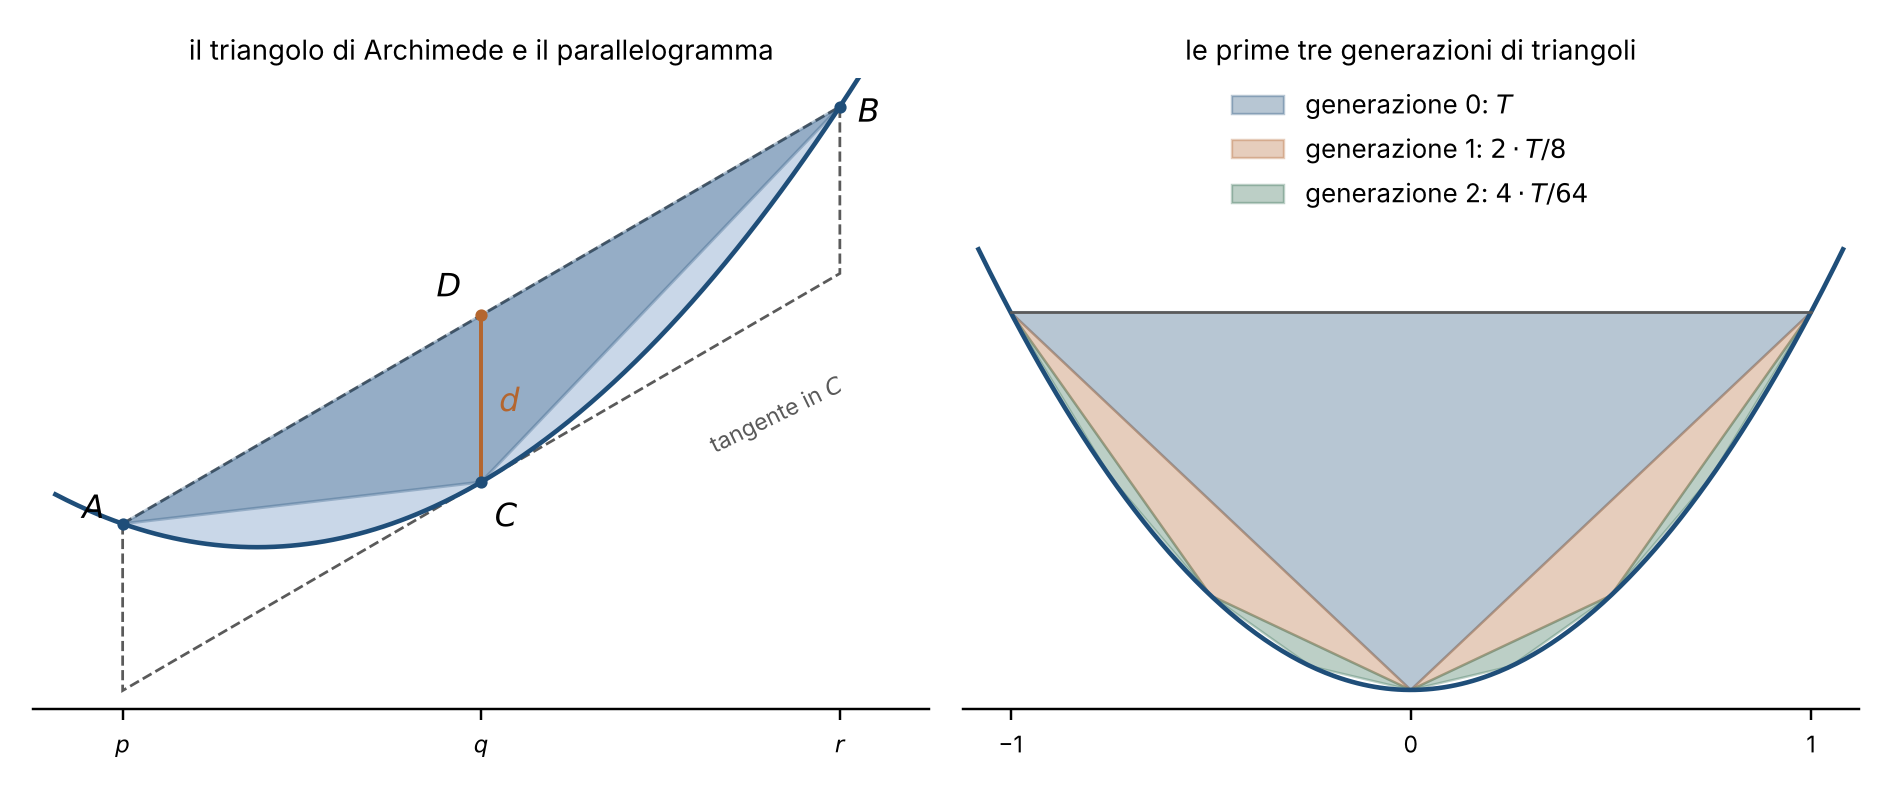
\includegraphics[width=\textwidth]{figure/archimede_parabola.png}
\caption{A sinistra, il segmento parabolico $\Sigma(p,r)$ (azzurro chiaro), il suo
triangolo di Archimede $ABC$ e il parallelogramma tratteggiato del
\cref{lem:triangolo-archimede}, delimitato dalla corda e dalla tangente in $C$, che
contiene il segmento e ha area doppia di quella del triangolo. A destra, i triangoli
delle prime tre generazioni per la corda di estremi $(\pm1,1)$: ogni generazione ha
area totale pari a $\frac14$ della precedente
(\texttt{python/fig\_archimede\_parabola.py}).}
\label{fig:archimede-parabola}
\end{figure}

\needspace{10\baselineskip}
Il segmento $\Sigma(p,r)$ si scompone nel triangolo $ABC$ e nei due segmenti
$\Sigma(p,q)$ e $\Sigma(q,r)$, di corde $AC$ e $CB$, senza punti interni comuni: per
$p\le x\le q$, ad esempio, la corda $AC$ divide il segmento verticale di $\Sigma(p,r)$
sopra $x$ in una parte che sta in $\Sigma(p,q)$ e una che sta nel triangolo. I due nuovi
segmenti hanno corde di larghezza $\frac w2$ e, per il lemma, triangoli di Archimede di
area $\frac18\cdot\frac{w^{3}}8$ ciascuno: insieme, un quarto del primo triangolo. È il
motore della dimostrazione.

\begin{proposizione}[Quadratura della parabola]\label{prop:quadratura-archimede}
Siano $p<r$ e sia $T=\frac{(r-p)^{3}}8$ l'area del triangolo di Archimede del segmento
parabolico $\Sigma(p,r)$. Se il segmento ha un'area, essa vale
\begin{equation}\label{eq:quadratura-archimede}
  \text{area }\Sigma(p,r)=\frac43\,T=\frac{(r-p)^{3}}6 .
\end{equation}
\end{proposizione}

\begin{schema}
\Ipotesi{$p<r$; \ l'area gode delle proprietà intuitive (aree elementari, additività,
confronto per inclusione).}
\Tesi{area $\Sigma(p,r)=\frac43\,T$, \ dove $T=\frac{(r-p)^{3}}8$ è l'area del
triangolo di Archimede.}
\end{schema}

\begin{strategia}
Si inscrivono nel segmento triangoli di generazioni successive: ogni generazione ha
area totale $\frac14$ della precedente, e l'unione delle prime $n+1$ generazioni è un
poligono la cui area è una somma geometrica finita, minore di $\frac43T$ per
$\frac T{3\cdot4^{n}}$. Ciò che resta scoperto è formato da segmenti più piccoli, e per
il \cref{lem:triangolo-archimede}(c) ha area al più doppia di quella della generazione
successiva. Archimede conclude con una \emph{doppia riduzione all'assurdo}: l'area del
segmento non può essere né maggiore né minore di $\frac43T$.
\end{strategia}

\begin{dimostrazione}
Sia $w=r-p$. Per $k\ge0$ intero, i punti $x_{j}=p+j\frac w{2^{k}}$,
$j=0,\dots,2^{k}$, dividono $[p,r]$ in $2^{k}$ parti uguali; chiamiamo \emph{segmenti di
generazione $k$} i $2^{k}$ segmenti parabolici $\Sigma(x_{j-1},x_{j})$, di corde di
larghezza $\frac w{2^{k}}$. Per il \cref{lem:triangolo-archimede}(b), ciascuno di essi
ha un triangolo di Archimede di area $\frac18\bigl(\frac w{2^{k}}\bigr)^{3}=\frac
T{8^{k}}$, e i triangoli di generazione $k$ hanno area totale
$2^{k}\cdot\frac T{8^{k}}=\frac T{4^{k}}$. Per la scomposizione descritta prima
dell'enunciato, ogni segmento di generazione $k$ è l'unione del suo triangolo e di due
segmenti di generazione $k+1$, senza punti interni comuni. Ripetendo la scomposizione,
per ogni $n\in\N$ il segmento $\Sigma(p,r)$ è l'unione del poligono $P_{n}$, formato dai
triangoli delle generazioni $0,1,\dots,n$, e dei $2^{n+1}$ segmenti di generazione
$n+1$, senza punti interni comuni.

\emph{L'area del poligono.} Per l'additività e per la somma della progressione
geometrica (\cref{prop:geometrica}) con $x=\frac14$,
\begin{equation}\label{eq:poligono-archimede}
  \text{area }P_{n}=T\Bigl(1+\frac14+\dots+\frac1{4^{n}}\Bigr)
  =T\,\frac{1-\frac1{4^{n+1}}}{1-\frac14}=\frac43\,T-\frac T{3\cdot4^{n}} .
\end{equation}

\emph{Ciò che resta scoperto.} Per il \cref{lem:triangolo-archimede}(c) e il confronto
per inclusione, ogni segmento di generazione $n+1$ ha area minore o uguale del doppio
del suo triangolo, cioè di $\frac{2T}{8^{n+1}}$. Sommando sui $2^{n+1}$ segmenti, la parte
scoperta $R_{n}=\text{area }\Sigma(p,r)-\text{area }P_{n}$ verifica
\begin{equation}\label{eq:resto-archimede}
  R_{n}\le2^{n+1}\cdot\frac{2T}{8^{n+1}}=\frac{2T}{4^{n+1}}=\frac T{2\cdot4^{n}} .
\end{equation}

\emph{La doppia riduzione all'assurdo.} Poniamo $\mathcal A=\text{area }\Sigma(p,r)$ e
$K=\frac43T$. Osserviamo che $4^{n}=(1+3)^{n}\ge1+3n>n$ per la disuguaglianza di
Bernoulli (\cref{teo:bernoulli}). Se fosse $\mathcal A>K$, per la proprietà di
Archimede (\cref{teo:archimede}) esisterebbe $n\in\N$ con $n>\frac T{2(\mathcal A-K)}$;
per la \eqref{eq:resto-archimede} si avrebbe $R_{n}\le\frac T{2\cdot4^{n}}<\frac T{2n}
<\mathcal A-K$, cioè $\text{area }P_{n}=\mathcal A-R_{n}>K$, contro la
\eqref{eq:poligono-archimede}, che dà $\text{area }P_{n}<K$. Se fosse $\mathcal A<K$,
esisterebbe $n\in\N$ con $n>\frac T{3(K-\mathcal A)}$, e per la
\eqref{eq:poligono-archimede} $K-\text{area }P_{n}=\frac T{3\cdot4^{n}}<\frac T{3n}<
K-\mathcal A$, cioè $\text{area }P_{n}>\mathcal A$: impossibile, perché il poligono $P_{n}$
è contenuto nel segmento. Esclusi i due casi, resta $\mathcal A=K=\frac43T$, e
$\frac43\cdot\frac{(r-p)^{3}}8=\frac{(r-p)^{3}}6$.
\end{dimostrazione}

\begin{osservazione}[La somma di Archimede e la serie geometrica]
\label{oss:somma-archimede}
Archimede ottenne la \eqref{eq:poligono-archimede} con una somma telescopica: ogni
termine, aumentato di un suo terzo, è un terzo del precedente,
$\frac1{4^{k}}+\frac13\cdot\frac1{4^{k}}=\frac13\cdot\frac1{4^{k-1}}$, e sommando per
$k=1,\dots,n$ si ha $1+\frac14+\dots+\frac1{4^{n}}+\frac13\cdot\frac1{4^{n}}=\frac43$.
Nel linguaggio del \cref{cap:serie}, la serie geometrica $1+\frac14+\frac1{16}+\cdots$
ha somma $\frac43$: la doppia riduzione all'assurdo fa le veci del passaggio al limite.
\end{osservazione}

\begin{esempio}[Due verifiche con il settore di parabola]\label{es:archimede-settore}
Per la corda di estremi $(\pm b,b^{2})$ la \eqref{eq:quadratura-archimede} dà
$\frac{(2b)^{3}}6=\frac43b^{3}$; con la \eqref{eq:area-parabola}, il segmento è il
rettangolo $[-b,b]\times[0,b^{2}]$ privato di due regioni congruenti al settore
\eqref{eq:settore-parabola}, e ha area $2b^{3}-2\cdot\frac{b^{3}}3=\frac43b^{3}$. Per la
corda di estremi $(0,0)$ e $(b,b^{2})$ si ottiene $\frac{b^{3}}6$, e infatti togliendo
il settore $S$ dal triangolo di vertici $(0,0)$, $(b,0)$, $(b,b^{2})$ resta
$\frac{b^{3}}2-\frac{b^{3}}3=\frac{b^{3}}6$. I triangoli di Archimede e i rettangoli
delle somme integrali portano allo stesso risultato.
\end{esempio}

\begin{notastorica}[Il \emph{Metodo} di Archimede]
La \emph{Quadratura della parabola}, indirizzata all'astronomo Dositeo di Pelusio,
contiene due dimostrazioni del teorema dei $\frac43$: una «meccanica», che equilibra il
segmento con un triangolo su una bilancia ideale, e quella con i triangoli inscritti che
abbiamo appena seguito. Entrambe, però, presuppongono di conoscere il risultato:
l'esaustione è un metodo di dimostrazione, non di scoperta, e già nel Seicento si
sospettava che Archimede possedesse un procedimento segreto per trovare i suoi teoremi.
La risposta arrivò nel 1906, quando il filologo danese Johan Ludvig Heiberg riconobbe, in
un libro di preghiere conservato a Costantinopoli, il testo raschiato di un codice di
opere di Archimede copiato nel \textsc{x} secolo, la cui pergamena era stata riutilizzata
nel 1229. Vi si trovava, in copia unica, il \emph{Metodo sui teoremi meccanici}, una
lettera a Eratostene in cui Archimede racconta di aver scoperto i suoi risultati
scomponendo le figure in infinite strisce parallele e bilanciandole su una leva, e
avverte che questo modo di ragionare suggerisce la verità ma non la dimostra. Il primo
esempio della lettera è proprio il segmento di parabola. Rimasto a lungo irreperibile,
il palinsesto ricomparve a un'asta nel 1998 ed è stato poi studiato a Baltimora con
tecniche di imaging multispettrale, che hanno restituito passi che Heiberg non era
riuscito a leggere. Le strisce del \emph{Metodo} sono le antenate degli indivisibili di
Cavalieri e dei rettangoli delle nostre somme integrali.
\end{notastorica}

%% ----------------------------------------------------------------------------
%%  §8.2  Somme integrali e integrale definito
%% ----------------------------------------------------------------------------
\section{Somme integrali e integrale definito}
\label{sec:integrale-definito}

Generalizziamo il procedimento del paragrafo precedente a una funzione qualsiasi,
purché \emph{limitata}. In tutto il paragrafo $[a,b]$ è un intervallo chiuso e limitato,
con $a<b$, e $f:[a,b]\to\R$ è una funzione limitata: esistono due costanti $m$, $M$ tali
che
\begin{equation}\label{eq:f-limitata}
  m\le f(x)\le M \qquad\perogni x\in[a,b] .
\end{equation}
Rispetto al settore di parabola cambiano due cose. La suddivisione dell'intervallo non
sarà più necessariamente in parti uguali; e, poiché $f$ non è più monotòna, l'altezza
dei rettangoli inscritti e circoscritti non sarà più il valore di $f$ in un estremo,
ma l'estremo inferiore e l'estremo superiore di $f$ nell'intervallo.

\subsection{Partizioni e somme integrali}

\begin{definizione}[Partizione]\label{def:partizione}\index{partizione}
Si chiama \emph{partizione} dell'intervallo $[a,b]$ un insieme finito
$P=\set{x_{0},x_{1},\dots,x_{n}}$ di punti, con $n\in\N$, tali che
\begin{equation}\label{eq:partizione}
  a=x_{0}<x_{1}<\dots<x_{k-1}<x_{k}<\dots<x_{n}=b .
\end{equation}
Gli $n+1$ punti individuano $n$ intervalli $I_{k}=[x_{k-1},x_{k}]$, $k=1,\dots,n$, di
ampiezza $\Delta x_{k}=x_{k}-x_{k-1}$. Il numero $\abs P=\max_{k}\Delta x_{k}$ si chiama
\emph{ampiezza} della partizione. Se $P$ e $Q$ sono partizioni di $[a,b]$ e
$P\subseteq Q$, si dice che $Q$ è \emph{più fine} di $P$, o che è un
\emph{raffinamento} di $P$.
\end{definizione}

Le ampiezze degli intervalli hanno per somma la lunghezza dell'intervallo:
$\sum_{k=1}^{n}\Delta x_{k}=x_{n}-x_{0}=b-a$ (ancora una somma telescopica). L'esempio
più semplice è la \emph{partizione uniforme} in $n$ parti uguali, con
$x_{k}=a+k\frac{b-a}n$ e $\abs P=\frac{b-a}n$, che abbiamo usato nel paragrafo
precedente. Se $P$ e $Q$ sono due partizioni di $[a,b]$, l'insieme
\begin{equation}\label{eq:unione-partizioni}
  R=P\cup Q ,
\end{equation}
ottenuto prendendo insieme i punti di $P$ e quelli di $Q$ (e ordinandoli), è ancora una
partizione di $[a,b]$, più fine sia di $P$ sia di $Q$.

\begin{definizione}[Somme integrali]\label{def:somme-integrali}\index{somma integrale}
Sia $P=\set{x_{0},\dots,x_{n}}$ una partizione di $[a,b]$. Per $k=1,\dots,n$ poniamo
\begin{equation}\label{eq:mk-Mk}
\begin{aligned}
  m_{k}&=\inf\set{f(x) \tc x\in[x_{k-1},x_{k}]},\\
  M_{k}&=\sup\set{f(x) \tc x\in[x_{k-1},x_{k}]} .
\end{aligned}
\end{equation}
Si chiamano \emph{somma integrale inferiore} e \emph{somma integrale superiore} di $f$
relative a $P$ i numeri
\begin{equation}\label{eq:somme-integrali}
  s(P)=\sum_{k=1}^{n}m_{k}\,(x_{k}-x_{k-1}), \qquad
  S(P)=\sum_{k=1}^{n}M_{k}\,(x_{k}-x_{k-1}) .
\end{equation}
Quando occorre ricordare la funzione si scrive $s(P,f)$ e $S(P,f)$.
\end{definizione}

Gli estremi $m_{k}$ e $M_{k}$ esistono finiti per il \cref{teo:esistenza-sup}, perché
l'insieme dei valori di $f$ in $[x_{k-1},x_{k}]$ è non vuoto e limitato; inoltre, per la
\eqref{eq:f-limitata}, $m\le m_{k}\le M_{k}\le M$. Moltiplicando per $\Delta x_{k}>0$ e
sommando si ottiene la stima
\begin{equation}\label{eq:stime-somme}
  m(b-a)\le s(P)\le S(P)\le M(b-a) \qquad\text{per ogni partizione } P .
\end{equation}
Se $f\ge0$, le somme integrali hanno il chiaro significato geometrico di somme delle
aree dei rettangoli rispettivamente inscritti nella regione sotto il grafico e
circoscritti a essa (\cref{fig:somme-integrali}). Si noti però che $s(P)$ e $S(P)$ sono
definite indipendentemente da ogni significato geometrico, anche se $f$ cambia segno.
Per $f(x)=x^{2}$ in $[0,b]$ e la partizione uniforme si ha $m_{k}=x_{k-1}^{2}$ e
$M_{k}=x_{k}^{2}$, e ritroviamo le somme $s_{n}$ e $S_{n}$ del \cref{sec:esaustione}.

\begin{figure}[htb]
\centering
\begin{tikzpicture}
\begin{axis}[width=0.9\textwidth, height=5.6cm, axis lines=left, xmin=0, xmax=4.95,
  ymin=0, ymax=3.1, xtick={0.3,1.3,2.5,3.3,4.5},
  xticklabels={$a=x_{0}$,$x_{1}$,$x_{2}$,$x_{3}$,$b=x_{4}$},
  ytick={1.345,2.424,2.733}, yticklabels={$m_{1}$,$m_{2}=M_{1}$,$M_{2}$},
  tick label style={font=\scriptsize}, clip=false]
  \fill[blu!20] (axis cs:0.3,0) rectangle (axis cs:1.3,1.345);
  \fill[blu!20] (axis cs:1.3,0) rectangle (axis cs:2.5,2.424);
  \fill[blu!20] (axis cs:2.5,0) rectangle (axis cs:3.3,1.899);
  \fill[blu!20] (axis cs:3.3,0) rectangle (axis cs:4.5,1.413);
  \draw[rame, thick] (axis cs:0.3,0) rectangle (axis cs:1.3,2.424);
  \draw[rame, thick] (axis cs:1.3,0) rectangle (axis cs:2.5,2.733);
  \draw[rame, thick] (axis cs:2.5,0) rectangle (axis cs:3.3,2.569);
  \draw[rame, thick] (axis cs:3.3,0) rectangle (axis cs:4.5,1.899);
  \addplot[curva, domain=0.2:4.65, samples=150] {1.7+0.8*sin(deg(1.3*x-0.9))+0.12*x};
  \addplot[tratteggio] coordinates {(0,1.345) (0.3,1.345)};
  \addplot[tratteggio] coordinates {(0,2.424) (1.3,2.424)};
  \addplot[tratteggio] coordinates {(0,2.733) (1.3,2.733)};
  \node[font=\scriptsize, blu, anchor=west] at (axis cs:4.67,1.53) {$y=f(x)$};
\end{axis}
\end{tikzpicture}
\caption{Somme integrali relative a una partizione non uniforme con $n=4$ intervalli.
L'area azzurra è la somma inferiore $s(P)$, quella racchiusa dai contorni in color rame
è la somma superiore $S(P)$. Nel secondo intervallo il massimo $M_{2}$ è assunto in un
punto interno, nel quarto il minimo $m_{4}$: le altezze dei rettangoli non sono, in
generale, i valori di $f$ negli estremi.}
\label{fig:somme-integrali}
\end{figure}

Il risultato seguente afferma che raffinando una partizione la somma inferiore
\emph{aumenta} (o resta uguale) e quella superiore \emph{diminuisce} (o resta uguale): le
due stime migliorano. Ne segue che \emph{ogni} somma inferiore è minore o uguale di
\emph{ogni} somma superiore, anche relativa a un'altra partizione.

\begin{lemma}[Raffinamento delle partizioni]\label{lem:raffinamento}
Siano $P$ e $Q$ partizioni di $[a,b]$.
\begin{enumerate}[label=\textup{(\alph*)}]
  \item Se $P\subseteq Q$, allora $s(P)\le s(Q)\le S(Q)\le S(P)$.
  \item In ogni caso, posto $R=P\cup Q$, risulta
  \begin{equation}\label{eq:s-minore-S}
    s(P)\le s(R)\le S(R)\le S(Q) .
  \end{equation}
\end{enumerate}
\end{lemma}

\begin{schema}
\Ipotesi{$f$ limitata in $[a,b]$; \ $P$, $Q$ partizioni di $[a,b]$.}
\Tesi{(a) $P\subseteq Q \implica s(P)\le s(Q)\le S(Q)\le S(P)$; \
(b) $s(P)\le S(Q)$ per ogni coppia $P$, $Q$.}
\end{schema}

\begin{strategia}
Il caso essenziale è quello in cui $Q$ ha un solo punto $\bar x$ in più di $P$. Allora
le due somme inferiori differiscono soltanto per i termini relativi all'intervallo di
$P$ che contiene $\bar x$, e tutto si riduce a un'osservazione sugli estremi inferiori:
l'estremo inferiore di $f$ su un insieme più piccolo è \emph{maggiore o uguale} di quello
sull'insieme più grande. Il caso generale si ottiene aggiungendo i punti di $Q$ uno alla
volta. La (b) segue dalla (a) applicata a $R$, che raffina sia $P$ sia $Q$.
\end{strategia}

\begin{dimostrazione}
(a) Supponiamo dapprima che $Q=P\cup\set{\bar x}$, con $x_{k-1}<\bar x<x_{k}$ per un certo
$k$, e poniamo
\[
  m'=\inf\set{f(x) \tc x\in[x_{k-1},\bar x]}, \qquad
  m''=\inf\set{f(x) \tc x\in[\bar x,x_{k}]} .
\]
Gli insiemi dei valori di $f$ in $[x_{k-1},\bar x]$ e in $[\bar x,x_{k}]$ sono contenuti
nell'insieme dei valori di $f$ in $[x_{k-1},x_{k}]$; poiché $m_{k}$ è un minorante di
quest'ultimo, è un minorante anche dei due sottoinsiemi, e quindi è minore o uguale dei
loro estremi inferiori: $m'\ge m_{k}$, $m''\ge m_{k}$. Le somme $s(Q)$ e $s(P)$ hanno in
comune tutti i termini tranne quelli relativi a $[x_{k-1},x_{k}]$, e dunque
\[
\begin{aligned}
  s(Q)-s(P)&=m'(\bar x-x_{k-1})+m''(x_{k}-\bar x)-m_{k}(x_{k}-x_{k-1})\\
  &\ge m_{k}\bigl[(\bar x-x_{k-1})+(x_{k}-\bar x)-(x_{k}-x_{k-1})\bigr]=0 .
\end{aligned}
\]
In modo analogo, gli estremi superiori sui due sottointervalli sono minori o uguali di
$M_{k}$, e si ottiene $S(Q)\le S(P)$. Se $Q$ contiene $p\ge2$ punti che non stanno in $P$,
si costruisce una catena $P=Q_{0}\subset Q_{1}\subset\dots\subset Q_{p}=Q$ in cui ciascuna
partizione si ottiene dalla precedente aggiungendo un solo punto; applicando il caso già
dimostrato a ogni anello della catena (cioè ragionando per induzione su $p$) si ottiene
$s(P)\le s(Q)$ e $S(Q)\le S(P)$. Infine $s(Q)\le S(Q)$ perché $m_{k}\le M_{k}$ per ogni
intervallo di $Q$.

(b) La partizione $R=P\cup Q$ è più fine sia di $P$ sia di $Q$. Applicando la (a) alla
coppia $P\subseteq R$ si ha $s(P)\le s(R)\le S(R)$, e applicandola alla coppia
$Q\subseteq R$ si ha $S(R)\le S(Q)$.
\end{dimostrazione}

\begin{figure}[htb]
\centering
\begin{tikzpicture}
\begin{axis}[width=0.62\textwidth, height=5cm, axis lines=left, xmin=0.4, xmax=4.1,
  ymin=0, ymax=4.3, xtick={1,2.4,3.6}, xticklabels={$x_{k-1}$,$\bar x$,$x_{k}$},
  ytick={0.85,2.04,3.84}, yticklabels={$m_{k}$,$m''=M'$,$M_{k}$},
  tick label style={font=\scriptsize}, clip=false]
  \fill[blu!20] (axis cs:1,0) rectangle (axis cs:3.6,0.85);
  \fill[verde!35] (axis cs:2.4,0.85) rectangle (axis cs:3.6,2.04);
  \fill[pattern=north east lines, pattern color=rame] (axis cs:1,2.04) rectangle
    (axis cs:2.4,3.84);
  \draw[rame, thick] (axis cs:1,0) rectangle (axis cs:3.6,3.84);
  \draw[grigio] (axis cs:2.4,0) -- (axis cs:2.4,3.84);
  \addplot[curva, domain=0.8:3.75, samples=80] {0.6+0.25*x^2};
  \addplot[tratteggio] coordinates {(0.4,2.04) (2.4,2.04)};
  \node[font=\scriptsize, verde!70!black] at (axis cs:3.0,1.45) {$+$};
  \node[font=\scriptsize, rame, fill=white, inner sep=1pt] at (axis cs:1.7,2.94) {$-$};
\end{axis}
\end{tikzpicture}
\caption{Aggiungendo il punto $\bar x$ all'intervallo $[x_{k-1},x_{k}]$, la somma
inferiore guadagna il rettangolo verde, perché in $[\bar x,x_{k}]$ l'estremo inferiore
sale da $m_{k}$ a $m''$; la somma superiore perde il rettangolo tratteggiato, perché in
$[x_{k-1},\bar x]$ l'estremo superiore scende da $M_{k}$ a $f(\bar x)=m''$.}
\label{fig:raffinamento}
\end{figure}

\subsection{L'integrale definito}

Indichiamo con $A$ l'insieme numerico costituito dalle somme inferiori $s(P)$, al variare
di $P$ tra tutte le partizioni di $[a,b]$, e con $B$ l'insieme delle corrispondenti somme
superiori:
\begin{equation}\label{eq:insiemi-A-B}
\begin{aligned}
  A&=\set{s(P) \tc P \text{ partizione di }[a,b]},\\
  B&=\set{S(P) \tc P \text{ partizione di }[a,b]} .
\end{aligned}
\end{equation}
Per il \cref{lem:raffinamento}(b), $a'\le b'$ per ogni $a'\in A$ e ogni $b'\in B$: i due
insiemi sono \emph{separati}. Per l'assioma di completezza (\cref{ass:completezza})
esiste almeno un numero reale $c$ maggiore o uguale di tutti gli elementi di $A$ e
minore o uguale di tutti gli elementi di $B$, cioè un \emph{elemento separatore}:
\[
  s(P)\le c\le S(Q) \qquad\text{per ogni coppia di partizioni } P, Q .
\]
In generale l'elemento separatore non è unico. Per descrivere tutti gli elementi
separatori introduciamo i numeri
\begin{equation}\label{eq:integrali-inf-sup}
\begin{aligned}
  s(f)&=\sup\set{s(P) \tc P \text{ partizione di }[a,b]},\\
  S(f)&=\inf\set{S(P) \tc P \text{ partizione di }[a,b]},
\end{aligned}
\end{equation}
detti rispettivamente \emph{integrale inferiore} e \emph{integrale superiore} di $f$.
Esistono finiti perché $A$ è non vuoto e limitato superiormente (da ogni elemento di
$B$), e $B$ è non vuoto e limitato inferiormente (da ogni elemento di $A$).

\begin{proposizione}[Gli elementi separatori]\label{prop:separatori}
Risulta $s(f)\le S(f)$, e un numero $c$ è elemento separatore tra $A$ e $B$ se e solo se
$s(f)\le c\le S(f)$.
\end{proposizione}

\begin{schema}
\Ipotesi{$f$ limitata in $[a,b]$; \ $A$, $B$ come in \eqref{eq:insiemi-A-B}.}
\Tesi{$s(f)\le S(f)$; \ gli elementi separatori sono tutti e soli i numeri
dell'intervallo $[s(f),S(f)]$.}
\end{schema}

\begin{strategia}
Tutto discende dalla definizione di estremo superiore come \emph{minimo dei maggioranti}
e di estremo inferiore come \emph{massimo dei minoranti}: un elemento separatore è un
maggiorante di $A$ che è anche un minorante di $B$.
\end{strategia}

\begin{dimostrazione}
Ogni elemento $S(Q)$ di $B$ è un maggiorante di $A$, e quindi è maggiore o uguale del
minimo dei maggioranti: $s(f)\le S(Q)$ per ogni $Q$. Dunque $s(f)$ è un minorante di $B$,
e quindi è minore o uguale del massimo dei minoranti: $s(f)\le S(f)$. Inoltre $c$ è
elemento separatore se e solo se è un maggiorante di $A$ e un minorante di $B$, cioè se
e solo se $c\ge\sup A=s(f)$ e $c\le\inf B=S(f)$.
\end{dimostrazione}

\begin{figure}[htb]
\centering
\begin{tikzpicture}[scale=1]
  \draw[-Latex, grigio] (0,1.1) -- (9.4,1.1);
  \foreach \x in {0.5,1.4,2.2,2.9,3.4,3.75,3.95} \fill[blu] (\x,1.1) circle (1.6pt);
  \foreach \x in {8.7,7.6,6.5,5.6,5.0,4.6,4.35} \fill[rame] (\x,1.1) circle (1.6pt);
  \draw[verde, very thick] (4.15,0.95) -- (4.15,1.25);
  \node[font=\scriptsize, above] at (4.15,1.25) {$s(f)=S(f)$};
  \node[font=\scriptsize, blu, below] at (2.0,1.0) {somme inferiori $s(P)$};
  \node[font=\scriptsize, rame, below] at (6.6,1.0) {somme superiori $S(P)$};
  \node[font=\scriptsize, anchor=west] at (9.5,1.1) {$f$ integrabile};
  \draw[-Latex, grigio] (0,0) -- (9.4,0);
  \foreach \x in {0.5,1.3,1.9,2.4,2.75,2.95,3.05} \fill[blu] (\x,0) circle (1.6pt);
  \foreach \x in {8.7,7.9,7.0,6.3,5.85,5.6,5.5} \fill[rame] (\x,0) circle (1.6pt);
  \draw[verde, very thick] (3.2,-0.15) -- (3.2,0.15);
  \draw[verde, very thick] (5.35,-0.15) -- (5.35,0.15);
  \fill[verde!25] (3.2,-0.06) rectangle (5.35,0.06);
  \node[font=\scriptsize, below] at (3.2,-0.15) {$s(f)$};
  \node[font=\scriptsize, below] at (5.35,-0.15) {$S(f)$};
  \node[font=\scriptsize, anchor=west] at (9.5,0) {$f$ non integrabile};
\end{tikzpicture}
\caption{In alto, le somme inferiori e quelle superiori si addensano attorno a un unico
elemento separatore: $f$ è integrabile. In basso, tra le une e le altre resta un
intervallo $[s(f),S(f)]$ di elementi separatori: $f$ non è integrabile.}
\label{fig:separatori}
\end{figure}

\begin{definizione}[Integrale definito secondo Riemann]\label{def:integrale}
\index{integrale definito}\index{funzione!integrabile}
Si dice che la funzione limitata $f$ è \emph{integrabile secondo Riemann} in $[a,b]$ se
esiste un \emph{unico} elemento separatore tra gli insiemi $A$ e $B$ delle somme
inferiori e superiori, cioè se $s(f)=S(f)$. Tale elemento si chiama \emph{integrale
definito} di $f$ in $[a,b]$ e si indica con il simbolo
\begin{equation}\label{eq:integrale}
  \int_{a}^{b}f(x)\,dx=s(f)=S(f) ,
\end{equation}
che si legge «integrale da $a$ a $b$ di $f(x)$ in $dx$».
\end{definizione}

Il termine «definito» distingue questo integrale, che è un numero, dagli
\emph{integrali indefiniti} del prossimo capitolo, nei quali gli estremi $a$, $b$ non
sono fissati. Vediamo subito due esempi opposti.

\begin{esempio}[Funzioni costanti]\label{es:integrale-costante}
Se $f(x)=c$ per ogni $x\in[a,b]$, in ogni intervallo di ogni partizione si ha
$m_{k}=M_{k}=c$, e quindi $s(P)=S(P)=c\sum\Delta x_{k}=c(b-a)$ per ogni $P$. Gli insiemi
$A$ e $B$ si riducono entrambi al numero $c(b-a)$, che è l'unico elemento separatore:
\begin{equation}\label{eq:integrale-costante}
  \int_{a}^{b}c\,dx=c\,(b-a) .
\end{equation}
\end{esempio}

\begin{esempio}[Una funzione limitata non integrabile]\label{es:dirichlet-non-integrabile}
Consideriamo in $[0,1]$ la funzione di Dirichlet $D$ dell'\cref{oss:dirichlet}, che
vale $1$ nei razionali e $0$ negli irrazionali. Per la densità dei razionali e degli
irrazionali (\cref{teo:densita-Q,cor:densita-irrazionali}), ogni intervallo
$[x_{k-1},x_{k}]$, con $x_{k-1}<x_{k}$, contiene sia punti razionali sia punti
irrazionali, e quindi $m_{k}=0$, $M_{k}=1$. Ne segue
\[
  s(P)=0, \qquad S(P)=\sum_{k=1}^{n}\Delta x_{k}=1 \qquad\text{per ogni partizione } P,
\]
dunque $s(D)=0<1=S(D)$: ogni numero di $[0,1]$ è un elemento separatore, e $D$ non è
integrabile secondo Riemann. La limitatezza, da sola, non basta all'integrabilità.
\end{esempio}

\subsection{Il criterio di integrabilità}

Verificare l'integrabilità calcolando $s(f)$ e $S(f)$, cioè un estremo superiore e un
estremo inferiore su \emph{tutte} le partizioni, è in genere impraticabile. Il teorema
seguente riduce il problema alla ricerca di \emph{una sola} partizione per ogni
tolleranza assegnata.

\begin{teorema}[Criterio di integrabilità]\label{teo:criterio-integrabilita}
\index{criterio!di integrabilità}
Una funzione $f$ limitata in $[a,b]$ è integrabile secondo Riemann in $[a,b]$ se e solo
se per ogni $\epsilon>0$ esiste una partizione $P$ di $[a,b]$ tale che
\begin{equation}\label{eq:criterio-integrabilita}
  S(P)-s(P)<\epsilon .
\end{equation}
\end{teorema}

\begin{schema}
\Ipotesi{$f$ limitata in $[a,b]$.}
\Tesi{$f$ integrabile $\sse$ $\perogni\epsilon>0\ \esiste P$ : $S(P)-s(P)<\epsilon$.}
\end{schema}

\begin{strategia}
\emph{Necessità}: se $s(f)=S(f)$, per le proprietà caratteristiche dell'estremo superiore
e dell'estremo inferiore esistono una somma inferiore e una somma superiore vicine a
meno di $\frac\epsilon2$ al valore comune, eventualmente relative a partizioni diverse
$P$ e $Q$; la partizione $R=P\cup Q$ le migliora entrambe (\cref{lem:raffinamento}).
\emph{Sufficienza}: $s(f)$ e $S(f)$ sono intrappolati tra $s(P)$ e $S(P)$, quindi distano
meno di $\epsilon$; un numero non negativo minore di ogni $\epsilon>0$ è nullo.
\end{strategia}

\begin{dimostrazione}
\emph{Necessità.} Sia $f$ integrabile, cioè $s(f)=S(f)$, e sia $\epsilon>0$. Per la
caratterizzazione dell'estremo superiore (\cref{prop:caratt-sup}) esiste una partizione
$P$ con $s(f)-\frac\epsilon2<s(P)$, e per quella dell'estremo inferiore
\eqref{eq:caratt-inf} esiste una partizione $Q$ con $S(Q)<S(f)+\frac\epsilon2$. Posto
$R=P\cup Q$, per la \eqref{eq:s-minore-S}
\[
  s(f)-\frac\epsilon2<s(P)\le s(R)\le S(R)\le S(Q)<S(f)+\frac\epsilon2 ,
\]
e quindi, essendo $s(f)=S(f)$,
\[
  S(R)-s(R)<\Bigl(S(f)+\frac\epsilon2\Bigr)-\Bigl(s(f)-\frac\epsilon2\Bigr)=\epsilon .
\]
La partizione cercata è $R$.

\emph{Sufficienza.} Per ogni partizione $P$ si ha $s(P)\le s(f)$, perché $s(f)$ è un
maggiorante delle somme inferiori, e $S(f)\le S(P)$, perché $S(f)$ è un minorante delle
somme superiori. Insieme alla \cref{prop:separatori} si ottiene
$s(P)\le s(f)\le S(f)\le S(P)$, e quindi
\[
  0\le S(f)-s(f)\le S(P)-s(P) .
\]
Se vale l'ipotesi, per ogni $\epsilon>0$ possiamo scegliere $P$ in modo che il secondo
membro sia minore di $\epsilon$: il numero $S(f)-s(f)$, che non dipende da $\epsilon$, è
non negativo e minore di ogni numero positivo, e dunque è nullo. Perciò $s(f)=S(f)$, cioè
$f$ è integrabile.
\end{dimostrazione}

Nella pratica il criterio si usa quasi sempre attraverso una successione di partizioni,
come abbiamo fatto per la parabola.

\begin{corollario}[Integrale come limite di somme]\label{cor:limite-somme}
Sia $f$ limitata in $[a,b]$ e sia $P_{n}$ una successione di partizioni di $[a,b]$ tale
che $S(P_{n})-s(P_{n})\to0$. Allora $f$ è integrabile e
\begin{equation}\label{eq:limite-somme}
  \int_{a}^{b}f(x)\,dx=\lim_{n\to+\infty}s(P_{n})=\lim_{n\to+\infty}S(P_{n}) .
\end{equation}
\end{corollario}

\begin{schema}
\Ipotesi{$f$ limitata in $[a,b]$; \ $S(P_{n})-s(P_{n})\to0$.}
\Tesi{$f$ integrabile; \ $s(P_{n})\to\int_{a}^{b}f$ e $S(P_{n})\to\int_{a}^{b}f$.}
\end{schema}

\begin{strategia}
L'integrabilità è il criterio appena dimostrato. Poi l'integrale, come ogni elemento
separatore, sta tra $s(P_{n})$ e $S(P_{n})$, e il teorema dei carabinieri fa il resto.
\end{strategia}

\begin{dimostrazione}
Dato $\epsilon>0$, per la definizione di limite esiste $n$ con
$S(P_{n})-s(P_{n})<\epsilon$, e per il \cref{teo:criterio-integrabilita} $f$ è
integrabile. Posto $I=\int_{a}^{b}f(x)\,dx$, si ha $s(P_{n})\le I\le S(P_{n})$, quindi
\[
  0\le I-s(P_{n})\le S(P_{n})-s(P_{n}), \qquad 0\le S(P_{n})-I\le S(P_{n})-s(P_{n}) ,
\]
e per il teorema dei carabinieri (\cref{teo:carabinieri}) $I-s(P_{n})\to0$ e
$S(P_{n})-I\to0$.
\end{dimostrazione}

\begin{esempio}[Gli integrali di $x$ e di $x^{2}$]\label{es:integrale-x-x2}
Sia $f(x)=x$ in $[0,b]$, e sia $P_{n}$ la partizione uniforme con $x_{k}=\frac{kb}n$.
Poiché $f$ è crescente, $m_{k}=x_{k-1}$ e $M_{k}=x_{k}$; con la somma dei primi
$n$ numeri naturali (\cref{prop:gauss}),
\[
\begin{aligned}
  S(P_{n})&=\frac bn\sum_{k=1}^{n}\frac{kb}n=\frac{b^{2}}{n^{2}}\cdot\frac{n(n+1)}2
  =\frac{b^{2}}2\cdot\frac{n+1}n,\\
  s(P_{n})&=\frac{b^{2}}2\cdot\frac{n-1}n ,
\end{aligned}
\]
e $S(P_{n})-s(P_{n})=\frac{b^{2}}n\to0$. Per il \cref{cor:limite-somme}
\begin{equation}\label{eq:integrale-x}
  \int_{0}^{b}x\,dx=\frac{b^{2}}2 ,
\end{equation}
che è l'area del triangolo di vertici $(0,0)$, $(b,0)$, $(b,b)$, come deve essere. Allo
stesso modo, le somme \eqref{eq:Sn-parabola}--\eqref{eq:sn-parabola} del settore di
parabola hanno differenza $\frac{b^{3}}n\to0$, e quindi
\begin{equation}\label{eq:integrale-x2}
  \int_{0}^{b}x^{2}\,dx=\frac{b^{3}}3 .
\end{equation}
\end{esempio}

Per una funzione non monotòna il calcolo di $m_{k}$ e $M_{k}$ richiede un po' più di
lavoro. Se $f$ è derivabile, però, gli strumenti del \cref{cap:applicazioni-derivate}
bastano: in ogni intervallo $[x_{k-1},x_{k}]$ la funzione, continua, ha massimo e minimo
(\cref{teo:weierstrass}), e se uno di essi è assunto in un punto interno, lì la derivata
si annulla (\cref{teo:fermat}). Dunque $m_{k}$ e $M_{k}$ vanno cercati tra i valori negli
estremi e quelli nei punti critici interni. Il programma seguente applica questa
osservazione a $f(x)=x^{3}-3x$ in $[-2,2]$, i cui punti critici sono $\pm1$.

\begin{python}[Somme integrali di una funzione non monotòna]
def darboux(f, a, b, n, critici=()):
    """Somme s(P), S(P) per la partizione uniforme in n parti:
    m_k e M_k si cercano tra gli estremi dell'intervallo e i
    punti critici interni (Weierstrass + Fermat)."""
    x = [a + k * (b - a) / n for k in range(n + 1)]
    s = S = 0.0
    for k in range(1, n + 1):
        cand = [x[k - 1], x[k]]
        cand += [c for c in critici if x[k - 1] < c < x[k]]
        v = [f(t) for t in cand]
        s += min(v) * (x[k] - x[k - 1])
        S += max(v) * (x[k] - x[k - 1])
    return s, S

f = lambda x: x**3 - 3 * x            # punti critici: -1 e 1
for n in (3, 30, 300, 3000):
    s, S = darboux(f, -2, 2, n, critici=(-1, 1))
    print(f"n = {n:4d}: s = {s:9.5f}  S = {S:8.5f}"
          f"  S-s = {S - s:8.5f}  n(S-s) = {n * (S - s):5.2f}")
\end{python}
\begin{risultato}
n =    3: s =  -7.60494  S =  7.60494  S-s = 15.20988  n(S-s) = 45.63
n =   30: s =  -0.79826  S =  0.79826  S-s =  1.59652  n(S-s) = 47.90
n =  300: s =  -0.08000  S =  0.08000  S-s =  0.16000  n(S-s) = 48.00
n = 3000: s =  -0.00800  S =  0.00800  S-s =  0.01600  n(S-s) = 48.00
\end{risultato}

Le due somme si stringono attorno a $0$, il valore suggerito dalla simmetria ($f$ è
dispari, e le aree sopra e sotto l'asse si compensano), e la differenza decresce come
$1/n$. Il prodotto $n(S-s)$ si stabilizza intorno a $48$, e il motivo è semplice: $f$
sale da $-2$ a $2$ in $[-2,-1]$, scende a $-2$ in $[-1,1]$ e risale a $2$ in $[1,2]$;
in ogni intervallo $M_{k}-m_{k}$ è al più la variazione totale di $f$ in
quell'intervallo (la somma delle sue salite e delle sue discese), e la somma di tutte le
salite e discese in $[-2,2]$ è $4+4+4=12$. Quindi
$S-s=\sum(M_{k}-m_{k})\frac4n\le\frac{48}n$.

\subsection{Significato geometrico e notazioni}

\begin{definizione}[Rettangoloide]\label{def:rettangoloide}\index{rettangoloide}
Sia $f\ge0$ in $[a,b]$. L'insieme
\begin{equation}\label{eq:rettangoloide}
  R_{f}=\set{(x,y)\in\R^{2} \tc a\le x\le b,\ 0\le y\le f(x)}
\end{equation}
si chiama \emph{rettangoloide} (o \emph{trapezoide}) di base $[a,b]$ relativo a $f$.
\end{definizione}

Per ogni partizione $P$, la somma $s(P)$ è l'area di un plurirettangolo contenuto in
$R_{f}$, e $S(P)$ quella di un plurirettangolo che contiene $R_{f}$
(\cref{fig:somme-integrali}). Il criterio di integrabilità afferma che, se $f$ è
integrabile, si possono trovare un plurirettangolo contenuto in $R_{f}$ e uno che lo
contiene le cui aree differiscono per meno di un qualsiasi $\epsilon>0$ assegnato. È
dunque ragionevole \emph{definire} l'area del rettangoloide come l'unico numero che
separa le aree dei plurirettangoli inscritti da quelle dei plurirettangoli
circoscritti:
\begin{equation}\label{eq:area-rettangoloide}
  \text{area }R_{f}=\int_{a}^{b}f(x)\,dx \qquad (f\ge0 \text{ integrabile}) .
\end{equation}
La definizione è coerente con le aree elementari: per una funzione costante si ottiene
l'area del rettangolo, per $f(x)=x$ quella del triangolo, per $f(x)=x^{2}$ quella del
settore di parabola calcolata da Archimede. È il punto di partenza della teoria della
misura delle figure piane di Peano e Jordan.

Nella scrittura $\int_{a}^{b}f(x)\,dx$ i numeri $a$ e $b$ si chiamano \emph{estremi di
integrazione}, la funzione $f$ \emph{funzione integranda}, la variabile $x$
\emph{variabile di integrazione}. Il risultato è un numero e non dipende da $x$, che è
una variabile «muta», come l'indice di una sommatoria: $\int_{a}^{b}f(x)\,dx$,
$\int_{a}^{b}f(t)\,dt$ e $\int_{a}^{b}f(s)\,ds$ indicano lo stesso numero. È utile
considerare l'integrale anche quando il primo estremo non è minore del secondo: si pone
\begin{equation}\label{eq:estremi-invertiti}
  \int_{a}^{b}f(x)\,dx=-\int_{b}^{a}f(x)\,dx \quad (a>b), \qquad
  \int_{a}^{a}f(x)\,dx=0 .
\end{equation}

\begin{osservazione}[Somme di Riemann]\label{oss:somme-riemann}\index{somma di Riemann}
Data una partizione $P$, scegliamo in ciascun intervallo $[x_{k-1},x_{k}]$ un punto
$\xi_{k}$ arbitrario e formiamo la \emph{somma di Riemann}
\begin{equation}\label{eq:somma-riemann}
  \sigma(P,\xi)=\sum_{k=1}^{n}f(\xi_{k})\,(x_{k}-x_{k-1}) .
\end{equation}
Poiché $m_{k}\le f(\xi_{k})\le M_{k}$, si ha $s(P)\le\sigma(P,\xi)\le S(P)$; se $f$ è
integrabile, anche l'integrale sta tra $s(P)$ e $S(P)$, e quindi
\begin{equation}\label{eq:riemann-stima}
  \Bigl|\sigma(P,\xi)-\int_{a}^{b}f(x)\,dx\Bigr|\le S(P)-s(P) .
\end{equation}
Le somme di Riemann sono quelle che si calcolano in pratica, perché richiedono soltanto
valori di $f$ e non estremi inferiori e superiori: scegliendo come $\xi_{k}$ l'estremo
sinistro, l'estremo destro o il punto medio di ogni intervallo si ottengono le formule
dei rettangoli che studieremo nel \cref{sec:integrabilita-continue}. La notazione di
Leibniz ricorda proprio queste somme: il simbolo $\int$ è una «S» allungata, iniziale
di \emph{summa}, e $dx$ ricorda le ampiezze $\Delta x_{k}$.
\end{osservazione}

\begin{notastorica}[Leibniz, Cauchy, Riemann, Darboux]
Gottfried Wilhelm Leibniz introdusse il simbolo $\int$ in un manoscritto del 29 ottobre
1675, sostituendo l'abbreviazione \emph{omn.} (\emph{omnia}, la «somma di tutte» le
linee di una figura) con una S allungata, iniziale di \emph{summa}; fu poi Joseph
Fourier, intorno al 1820, a proporre di scrivere gli estremi in basso e in alto. Per i
successori di Leibniz, a partire da Johann Bernoulli ed Eulero, l'integrale divenne
soprattutto l'operazione inversa della derivazione. Il primo a definirlo in modo
autonomo, come limite di somme, fu Augustin-Louis Cauchy nel \emph{Résumé des leçons}
del 1823, per le funzioni continue e con le somme costruite sugli estremi sinistri: il
legame con la derivata, che per Leibniz era quasi una definizione, diventò così un
teorema, quello fondamentale del prossimo capitolo. Cauchy deduceva l'esistenza del
limite dal fatto che due somme relative a partizioni abbastanza fini differiscono poco,
un passaggio che richiede la completezza dei reali, allora non ancora formulata; inoltre
la somma dipende da tutta la partizione e non dalla sola ampiezza, e un limite «per
ampiezza tendente a zero» sfuggiva alle definizioni di limite note (per questo nel
\cref{teo:riemann-continue} useremo successioni di partizioni). Una teoria dei limiti
adatta a questi casi fu proposta solo nel 1922 da Eliakim H.~Moore e Herman L.~Smith.
Bernhard Riemann, nella dissertazione di abilitazione del 1854 sulle serie
trigonometriche (pubblicata postuma, a cura di Dedekind, nel 1867), si pose la domanda
dell'epigrafe e rispose con le somme \eqref{eq:somma-riemann} a punti $\xi_{k}$
arbitrari, ammettendo funzioni qualsiasi purché limitate; diede anche il criterio di
integrabilità. La formulazione con le somme inferiori e superiori, che abbiamo seguito,
è dovuta a Gaston Darboux (1875); le due definizioni sono equivalenti.
\end{notastorica}

\subsection{Approfondimento: l'integrale con le funzioni a scala}
\label{subsec:funzioni-scala}

Molti testi, tra cui \cite{giusti}, definiscono l'integrale in un modo che a prima vista
sembra diverso dal nostro: al posto delle somme inferiori e superiori usano le
\emph{funzioni a scala} che stanno sotto e sopra $f$. Mostriamo che le due definizioni
coincidono; la verifica richiede un po' di attenzione nei punti di suddivisione.

\begin{definizione}[Funzione a scala]\label{def:funzione-scala}\index{funzione!a scala}
Una funzione $\varphi:[a,b]\to\R$ si dice \emph{a scala} se esiste una partizione
$P=\set{x_{0},\dots,x_{n}}$ di $[a,b]$ tale che $\varphi$ è costante in ciascun
intervallo aperto $(x_{k-1},x_{k})$: $\varphi(x)=c_{k}$ per $x_{k-1}<x<x_{k}$. Una tale
partizione si dice \emph{adatta} a $\varphi$; i valori di $\varphi$ nei punti $x_{k}$
sono arbitrari. Il numero
\begin{equation}\label{eq:integrale-scala}
  I(\varphi)=\sum_{k=1}^{n}c_{k}\,(x_{k}-x_{k-1})
\end{equation}
si chiama \emph{integrale elementare} di $\varphi$.
\end{definizione}

Il numero $I(\varphi)$ non dipende dalla partizione adatta. Se si aggiunge a $P$ un
punto $\bar x\in(x_{k-1},x_{k})$, la partizione resta adatta e il termine
$c_{k}(x_{k}-x_{k-1})$ si spezza in $c_{k}(\bar x-x_{k-1})+c_{k}(x_{k}-\bar x)$, con la
stessa somma; aggiungendo i punti uno alla volta, come nel \cref{lem:raffinamento}, la
somma non cambia passando a un raffinamento. Se $P$ e $P'$ sono adatte, $P\cup P'$
raffina entrambe, e le tre somme coincidono. Se $f\ge0$ e $\varphi\le f$, $I(\varphi)$ è
l'area di un plurirettangolo contenuto nel rettangoloide di $f$, come una somma
inferiore.

Sia ora $f$ limitata in $[a,b]$, con $m\le f\le M$. Poniamo
\begin{equation}\label{eq:integrali-scala}
\begin{aligned}
  I_{-}(f)&=\sup\set{I(\psi) \tc \psi \text{ a scala},\ \psi\le f \text{ in }[a,b]},\\
  I^{+}(f)&=\inf\set{I(\varphi) \tc \varphi \text{ a scala},\ \varphi\ge f \text{ in }[a,b]} .
\end{aligned}
\end{equation}
Gli insiemi sono non vuoti, perché le costanti $m$ e $M$ sono funzioni a scala; e se
$\psi\le f$ è a scala, i suoi valori $c_{k}$ sono minori o uguali di $M$, quindi
$I(\psi)\le M(b-a)$. Analogamente $I(\varphi)\ge m(b-a)$, e i due numeri sono finiti.

\begin{proposizione}[Funzioni a scala e somme integrali]\label{prop:scala-darboux}
Se $f$ è limitata in $[a,b]$, allora $I_{-}(f)=s(f)$ e $I^{+}(f)=S(f)$. In particolare
$f$ è integrabile secondo Riemann se e solo se $I_{-}(f)=I^{+}(f)$, e in tal caso il
valore comune è $\int_{a}^{b}f(x)\,dx$.
\end{proposizione}

\begin{schema}
\Ipotesi{$f$ limitata in $[a,b]$, \ $m\le f\le M$.}
\Tesi{$I_{-}(f)=s(f)$ \ e \ $I^{+}(f)=S(f)$, \ con $I_{-}$, $I^{+}$ definiti dalla
\eqref{eq:integrali-scala}.}
\end{schema}

\begin{strategia}
Ogni somma inferiore è l'integrale elementare di una funzione a scala minorante:
quella che vale $m_{k}$ all'interno del $k$-esimo intervallo e coincide con $f$ nei punti
di suddivisione. Dunque $I_{-}(f)\ge s(f)$. Il viceversa è più delicato, perché una
funzione a scala minorante può superare $m_{k}$ all'interno di un intervallo, se $f$
assume valori piccoli soltanto negli estremi: si rimedia isolando i punti di
suddivisione in intervallini di ampiezza $\eta$, il cui contributo è proporzionale a
$\eta$. Per $I^{+}(f)$ basta passare a $-f$.
\end{strategia}

\begin{dimostrazione}
\emph{$I_{-}(f)\ge s(f)$.} Sia $P=\set{x_{0},\dots,x_{n}}$ una partizione, e sia
$\psi_{P}$ la funzione che vale $m_{k}$ in $(x_{k-1},x_{k})$ e $f(x_{k})$ nei punti
$x_{k}$. È una funzione a scala, con $P$ adatta, e $\psi_{P}\le f$: all'interno degli
intervalli perché $m_{k}$ è un minorante di $f$ in $[x_{k-1},x_{k}]$, nei punti di
suddivisione per costruzione. Dunque $s(P)=I(\psi_{P})\le I_{-}(f)$ per ogni $P$, e
passando all'estremo superiore $s(f)\le I_{-}(f)$.

\emph{$I_{-}(f)\le s(f)$.} Sia $\psi\le f$ a scala, con partizione adatta
$P=\set{x_{0},\dots,x_{n}}$ e valori $c_{k}$; come osservato, $c_{k}\le M$. Fissiamo
$\eta$ con $0<2\eta<\min_{k}\Delta x_{k}$ e sia $Q$ la partizione ottenuta aggiungendo a
$P$ i punti $x_{k-1}+\eta$ e $x_{k}-\eta$, per $k=1,\dots,n$. Ogni intervallo
$[x_{k-1},x_{k}]$ si divide così in due intervallini di ampiezza $\eta$ adiacenti agli
estremi e nell'intervallo centrale $J_{k}=[x_{k-1}+\eta,x_{k}-\eta]$. Poiché $J_{k}$ è
contenuto in $(x_{k-1},x_{k})$, dove $f\ge\psi=c_{k}$, l'estremo inferiore di $f$ in
$J_{k}$ è maggiore o uguale di $c_{k}$; negli intervallini è maggiore o uguale di $m$.
La partizione $Q$ è adatta a $\psi$, e con essa
\[
  I(\psi)=\sum_{k=1}^{n}\bigl(c_{k}\abs{J_{k}}+2c_{k}\eta\bigr), \qquad
  s(Q)\ge\sum_{k=1}^{n}\bigl(c_{k}\abs{J_{k}}+2m\eta\bigr),
\]
dove $\abs{J_{k}}$ è l'ampiezza di $J_{k}$. Sottraendo,
\[
  I(\psi)-s(Q)\le2\eta\sum_{k=1}^{n}(c_{k}-m)\le2n(M-m)\,\eta ,
\]
e quindi $I(\psi)\le s(f)+2n(M-m)\eta$. Qui $n$ dipende soltanto da $\psi$, mentre $\eta$
si può scegliere piccolo a piacere: il numero $I(\psi)-s(f)$ è minore o uguale di ogni
numero positivo, e quindi $I(\psi)\le s(f)$. Passando all'estremo superiore su $\psi$,
$I_{-}(f)\le s(f)$.

\emph{Integrali superiori.} Si ha $\varphi\ge f$ se e solo se $-\varphi\le-f$, e
$I(-\varphi)=-I(\varphi)$; quindi $I^{+}(f)=-I_{-}(-f)$. D'altra parte, in ogni
intervallo l'estremo inferiore di $-f$ è l'opposto dell'estremo superiore di $f$, per cui
$s(P,-f)=-S(P,f)$ e $s(-f)=-S(f)$. Applicando a $-f$ quanto già dimostrato,
$I^{+}(f)=-I_{-}(-f)=-s(-f)=S(f)$. L'ultima affermazione segue dalla
\cref{def:integrale}.
\end{dimostrazione}

\begin{osservazione}[Integrale delle funzioni a scala]\label{oss:integrale-scala}
Ogni funzione a scala $\varphi$ è integrabile, e $\int_{a}^{b}\varphi(x)\,dx=I(\varphi)$.
Infatti $\varphi$, che assume un numero finito di valori, è limitata, ed è minorante e
maggiorante di sé stessa; per la \eqref{eq:integrali-scala}, la
\cref{prop:scala-darboux} e la \cref{prop:separatori},
$I(\varphi)\le I_{-}(\varphi)=s(\varphi)\le S(\varphi)=I^{+}(\varphi)\le I(\varphi)$, e
tutte le disuguaglianze sono uguaglianze. Ad esempio, una funzione nulla tranne che in
un numero finito di punti è a scala, con integrale nullo: con la linearità del
\cref{sec:proprieta-integrale} si ritrova l'\cref{es:valore-in-un-punto}. Le due
definizioni sono dunque la stessa idea, l'\emph{unico elemento separatore}, vista con
due strumenti: le somme sulle partizioni o i plurirettangoli delle funzioni a scala.
\end{osservazione}

\begin{notastorica}[Il commerciante di Lebesgue]
Approssimare $f$ dal basso e dall'alto con funzioni costanti su intervalli è anche il
punto di partenza della teoria della misura. Giuseppe Peano nel 1887 e Camille Jordan
pochi anni dopo definirono la misura interna ed esterna di un insieme mediante i
plurirettangoli contenuti nell'insieme e quelli che lo contengono, come le somme
inferiori e superiori del rettangoloide; ma l'insieme dei razionali di $[0,1]$ ha misura
interna $0$ ed esterna $1$, e non è misurabile. Émile Borel, nel 1898, chiese alla misura
di essere additiva anche per successioni di insiemi disgiunti, e su questa base Henri
Lebesgue, nella tesi \emph{Intégrale, longueur, aire} (1902), costruì un integrale nuovo.
In una conferenza del 1926 ne spiegò l'idea con un'immagine: Riemann somma i valori di
$f$ nell'ordine in cui li incontra percorrendo l'intervallo, come un commerciante
disordinato che conta le monete nell'ordine in cui gli capitano in mano; Lebesgue
invece le raggruppa per valore, come il commerciante metodico che conta quante monete
ha di ciascun taglio. Si suddivide cioè l'insieme dei \emph{valori} di $f$, non
l'intervallo, e si approssima $f$ con funzioni costanti su insiemi più generali degli
intervalli, dei quali occorre conoscere la misura. Il guadagno non è soltanto una classe
più ampia di funzioni integrabili (la funzione di Dirichlet lo è, con integrale nullo),
ma soprattutto i teoremi di passaggio al limite sotto il segno di integrale, essenziali
per le serie di Fourier. Non tutti gli insiemi, però, sono misurabili: nel 1905
Giuseppe Vitali ne costruì uno che non lo è, servendosi dell'assioma della scelta,
formulato da Ernst Zermelo l'anno prima.
\end{notastorica}

%% ----------------------------------------------------------------------------
%%  §8.3  Proprietà degli integrali definiti
%% ----------------------------------------------------------------------------
\section{Proprietà degli integrali definiti}
\label{sec:proprieta-integrale}

Esaminiamo le proprietà fondamentali dell'integrale definito di una funzione
integrabile secondo Riemann in un intervallo chiuso e limitato. Molte hanno un chiaro
significato geometrico quando si interpretano gli integrali di funzioni positive come
aree; le dimostrazioni, però, non possono appoggiarsi a questo significato, perché
l'area del rettangoloide è stata \emph{definita} mediante l'integrale. Tutte poggiano
sul criterio di integrabilità e sul lemma di raffinamento. Cominciamo con uno strumento
che useremo più volte.

\subsection{L'oscillazione}

\begin{lemma}[Oscillazione]\label{lem:oscillazione}\index{oscillazione}
Sia $f$ limitata in un insieme non vuoto $I$, e siano $m_{I}=\inf_{I}f$,
$M_{I}=\sup_{I}f$. Allora
\begin{equation}\label{eq:oscillazione}
  M_{I}-m_{I}=\sup\set{\abs{f(x)-f(x')} \tc x,x'\in I} .
\end{equation}
Il numero \eqref{eq:oscillazione} si chiama \emph{oscillazione} di $f$ in $I$.
\end{lemma}

\begin{schema}
\Ipotesi{$f$ limitata in $I\neq\emptyset$.}
\Tesi{$\sup_{I}f-\inf_{I}f=\sup_{x,x'\in I}\abs{f(x)-f(x')}$.}
\end{schema}

\begin{strategia}
Una disuguaglianza è immediata: due valori di $f$ in $I$ stanno entrambi tra $m_{I}$ e
$M_{I}$, quindi distano al più $M_{I}-m_{I}$. Per l'altra, si scelgono due valori
$f(x)$ e $f(x')$ vicini quanto si vuole rispettivamente a $M_{I}$ e a $m_{I}$, come
permette la caratterizzazione degli estremi.
\end{strategia}

\begin{dimostrazione}
Sia $D$ l'insieme a secondo membro. Per $x,x'\in I$ si ha $m_{I}\le f(x)\le M_{I}$ e
$m_{I}\le f(x')\le M_{I}$, quindi $f(x)-f(x')\le M_{I}-m_{I}$ e
$f(x')-f(x)\le M_{I}-m_{I}$, cioè $\abs{f(x)-f(x')}\le M_{I}-m_{I}$: il numero
$M_{I}-m_{I}$ è un maggiorante di $D$, e quindi $\sup D\le M_{I}-m_{I}$. Viceversa, fissato
$\epsilon>0$, per le caratterizzazioni \eqref{eq:caratt-sup} e \eqref{eq:caratt-inf}
esistono $x,x'\in I$ con $f(x)>M_{I}-\frac\epsilon2$ e $f(x')<m_{I}+\frac\epsilon2$, e allora
$\abs{f(x)-f(x')}\ge f(x)-f(x')>M_{I}-m_{I}-\epsilon$. Dunque nessun numero
$M_{I}-m_{I}-\epsilon$ è un maggiorante di $D$, e $\sup D\ge M_{I}-m_{I}$.
\end{dimostrazione}

Indicando con $\omega_{k}=M_{k}-m_{k}$ l'oscillazione di $f$ nell'intervallo
$[x_{k-1},x_{k}]$ di una partizione $P$, la differenza tra le somme integrali si scrive
\begin{equation}\label{eq:S-s-oscillazioni}
  S(P)-s(P)=\sum_{k=1}^{n}\omega_{k}\,\Delta x_{k} ,
\end{equation}
una somma di termini non negativi: il criterio di integrabilità chiede che le
oscillazioni, pesate con le ampiezze degli intervalli, abbiano somma piccola.

\subsection{Additività rispetto all'intervallo}

\begin{lemma}[Integrabilità sui sottointervalli e sull'unione]\label{lem:sottointervallo}
\begin{enumerate}[label=\textup{(\alph*)}]
  \item Se $f$ è integrabile in $[a,b]$ e $[c,d]\subseteq[a,b]$, allora $f$ è integrabile
  in $[c,d]$.
  \item Se $a<c<b$ e $f$ è integrabile in $[a,c]$ e in $[c,b]$, allora $f$ è integrabile
  in $[a,b]$.
\end{enumerate}
\end{lemma}

\begin{schema}
\Ipotesi{(a) $f$ integrabile in $[a,b]$, $[c,d]\subseteq[a,b]$; \
(b) $f$ integrabile in $[a,c]$ e in $[c,b]$.}
\Tesi{(a) $f$ integrabile in $[c,d]$; \ (b) $f$ integrabile in $[a,b]$.}
\end{schema}

\begin{strategia}
Si usa il criterio di integrabilità con la scrittura \eqref{eq:S-s-oscillazioni}. Per la
(a), si aggiungono $c$ e $d$ a una partizione «buona» di $[a,b]$: i suoi intervalli
contenuti in $[c,d]$ formano una partizione di $[c,d]$, e la corrispondente somma di
termini non negativi è minore della somma totale. Per la (b), si uniscono due
partizioni «buone» dei due intervalli.
\end{strategia}

\begin{dimostrazione}
(a) Sia $\epsilon>0$. Per il \cref{teo:criterio-integrabilita} esiste una partizione $P$
di $[a,b]$ con $S(P)-s(P)<\epsilon$; per il \cref{lem:raffinamento} anche
$P'=P\cup\set{c,d}$ verifica $S(P')-s(P')<\epsilon$. I punti di $P'$ che stanno in
$[c,d]$ formano una partizione $P''$ di $[c,d]$, i cui intervalli sono intervalli di
$P'$, con gli stessi estremi inferiori e superiori di $f$. Per la
\eqref{eq:S-s-oscillazioni}, $S(P'')-s(P'')$ è una parte della somma di termini non
negativi che dà $S(P')-s(P')$, e quindi $S(P'')-s(P'')<\epsilon$. Per il criterio, $f$ è
integrabile in $[c,d]$.

(b) Sia $\epsilon>0$ e siano $P_{1}$, $P_{2}$ partizioni di $[a,c]$ e di $[c,b]$ con
$S(P_{i})-s(P_{i})<\frac\epsilon2$. L'insieme $P=P_{1}\cup P_{2}$ è una partizione di
$[a,b]$ i cui intervalli sono quelli di $P_{1}$ e quelli di $P_{2}$; quindi
\begin{equation}\label{eq:somme-unione}
  s(P)=s(P_{1})+s(P_{2}), \qquad S(P)=S(P_{1})+S(P_{2}),
\end{equation}
e $S(P)-s(P)<\epsilon$. Per il criterio, $f$ è integrabile in $[a,b]$.
\end{dimostrazione}

\begin{teorema}[Additività dell'integrale rispetto all'intervallo]\label{teo:additivita}
\index{integrale definito!additività}
Sia $f$ integrabile in un intervallo $[\alpha,\beta]$ e siano $a,b,c$ tre punti
qualsiasi di $[\alpha,\beta]$. Allora
\begin{equation}\label{eq:additivita}
  \int_{a}^{b}f(x)\,dx=\int_{a}^{c}f(x)\,dx+\int_{c}^{b}f(x)\,dx .
\end{equation}
\end{teorema}

\begin{schema}
\Ipotesi{$f$ integrabile in $[\alpha,\beta]$; \ $a,b,c\in[\alpha,\beta]$ (in ordine
qualsiasi).}
\Tesi{$\int_{a}^{b}f=\int_{a}^{c}f+\int_{c}^{b}f$.}
\end{schema}

\begin{strategia}
Gli integrali hanno senso per il \cref{lem:sottointervallo}(a), e, se gli estremi non
sono in ordine crescente, per le convenzioni \eqref{eq:estremi-invertiti}. Il caso
essenziale è $a<c<b$: unendo una partizione di $[a,c]$ e una di $[c,b]$, le somme
integrali si sommano \eqref{eq:somme-unione}, e i due membri della
\eqref{eq:additivita} risultano intrappolati in uno stesso intervallo, di ampiezza
piccola a piacere. Gli altri ordinamenti dei tre punti si riconducono a questo grazie
alle convenzioni, che sono state scelte proprio a questo scopo.
\end{strategia}

\begin{dimostrazione}
\emph{Caso $a<c<b$.} Per il \cref{lem:sottointervallo}(a), $f$ è integrabile in
$[a,b]$, in $[a,c]$ e in $[c,b]$. Sia $\epsilon>0$; per il criterio di integrabilità
esistono partizioni $P_{1}$ di $[a,c]$ e $P_{2}$ di $[c,b]$ con
$S(P_{i})-s(P_{i})<\frac\epsilon2$. Posto $P=P_{1}\cup P_{2}$, per la
\eqref{eq:somme-unione} e perché l'integrale sta tra ogni somma inferiore e ogni somma
superiore,
\[
  s(P_{1})+s(P_{2})=s(P)\le\int_{a}^{b}f(x)\,dx\le S(P)=S(P_{1})+S(P_{2}) .
\]
D'altra parte $s(P_{1})\le\int_{a}^{c}f\le S(P_{1})$ e $s(P_{2})\le\int_{c}^{b}f\le S(P_{2})$,
e sommando
\[
  s(P_{1})+s(P_{2})\le\int_{a}^{c}f(x)\,dx+\int_{c}^{b}f(x)\,dx\le S(P_{1})+S(P_{2}) .
\]
I due membri della \eqref{eq:additivita} appartengono dunque allo stesso intervallo
$[s(P),S(P)]$, di ampiezza minore di $\epsilon$, e distano meno di $\epsilon$. Poiché
$\epsilon>0$ è arbitrario, sono uguali.

\emph{Altri casi.} Se due dei tre punti coincidono, la tesi segue dalle convenzioni
\eqref{eq:estremi-invertiti}: ad esempio, per $c=a$ essa si riduce a
$\int_{a}^{b}f=0+\int_{a}^{b}f$, e per $b=a$ a $0=\int_{a}^{c}f+\int_{c}^{a}f$. Se i tre
punti sono distinti, ma non nell'ordine $a<c<b$, si applica il caso già dimostrato
ai tre punti riordinati. Ad esempio, se $c<a<b$, si ha
$\int_{c}^{b}f=\int_{c}^{a}f+\int_{a}^{b}f$, da cui
$\int_{a}^{b}f=\int_{c}^{b}f-\int_{c}^{a}f=\int_{a}^{c}f+\int_{c}^{b}f$; se $b<c<a$, dal
caso dimostrato $\int_{b}^{a}f=\int_{b}^{c}f+\int_{c}^{a}f$, e cambiando i segni si ottiene la
tesi. Tutti i casi si riassumono così: per le convenzioni
\eqref{eq:estremi-invertiti}, la \eqref{eq:additivita} equivale a
$\int_{a}^{b}f+\int_{b}^{c}f+\int_{c}^{a}f=0$, un'espressione che non cambia permutando
ciclicamente $a$, $b$, $c$ e cambia segno scambiandone due; se vale per una
disposizione dei tre punti, vale quindi per tutte.
\end{dimostrazione}

\begin{figure}[htb]
\centering
\begin{tikzpicture}
\begin{axis}[name=q1, width=0.5\textwidth, height=4.4cm, axis lines=left, xmin=0,
  xmax=4.5, ymin=0, ymax=2.6, xtick={0.6,2.1,3.9}, xticklabels={$a$,$c$,$b$},
  ytick=\empty]
  \addplot[draw=none, fill=blu!20, domain=0.6:3.9, samples=80]
    {1.3+0.5*sin(deg(1.4*x))+0.12*x} \closedcycle;
  \addplot[curva, domain=0.3:4.2, samples=80] {1.3+0.5*sin(deg(1.4*x))+0.12*x};
  \node[font=\small, blu] at (axis cs:2.25,0.7) {$A$};
\end{axis}
\begin{axis}[at={(q1.east)}, anchor=west, xshift=0.8cm, width=0.5\textwidth,
  height=4.4cm, axis lines=left, xmin=0, xmax=4.5, ymin=0, ymax=2.6,
  xtick={0.6,2.1,3.9}, xticklabels={$a$,$c$,$b$}, ytick=\empty]
  \addplot[draw=none, fill=blu!20, domain=0.6:2.1, samples=40]
    {1.3+0.5*sin(deg(1.4*x))+0.12*x} \closedcycle;
  \addplot[draw=none, fill=rame!25, domain=2.1:3.9, samples=40]
    {1.3+0.5*sin(deg(1.4*x))+0.12*x} \closedcycle;
  \addplot[curva, domain=0.3:4.2, samples=80] {1.3+0.5*sin(deg(1.4*x))+0.12*x};
  \addplot[grigio] coordinates {(2.1,0) (2.1,1.652)};
  \node[font=\small, blu] at (axis cs:1.35,0.7) {$A_{1}$};
  \node[font=\small, rame] at (axis cs:3.0,0.7) {$A_{2}$};
\end{axis}
\end{tikzpicture}
\caption{Additività: se $f\ge0$ e $a<c<b$, la \eqref{eq:additivita} afferma che l'area
del rettangoloide $A$ è la somma delle aree di $A_{1}$ e $A_{2}$, che non hanno punti
interni in comune.}
\label{fig:additivita}
\end{figure}

Il \cref{lem:sottointervallo}(b) ha una conseguenza pratica: per stabilire che una
funzione è integrabile si può spezzare l'intervallo in un numero finito di parti e
verificare l'integrabilità su ciascuna; l'integrale complessivo è poi la somma degli
integrali sulle parti, per la \eqref{eq:additivita}.

\subsection{Linearità}

\begin{teorema}[Linearità dell'integrale]\label{teo:linearita}
\index{integrale definito!linearità}
Se $f$ e $g$ sono integrabili in $[a,b]$ e $c\in\R$, anche $f+g$ e $cf$ sono integrabili
in $[a,b]$, e risulta
\begin{align}
  \int_{a}^{b}\bigl[f(x)+g(x)\bigr]dx&=\int_{a}^{b}f(x)\,dx+\int_{a}^{b}g(x)\,dx ;
  \label{eq:linearita-somma}\\
  \int_{a}^{b}c\,f(x)\,dx&=c\int_{a}^{b}f(x)\,dx .
  \label{eq:linearita-prodotto}
\end{align}
\end{teorema}

\begin{schema}
\Ipotesi{$f$, $g$ integrabili in $[a,b]$; \ $c\in\R$.}
\Tesi{$f+g$ e $cf$ integrabili; \ $\int(f+g)=\int f+\int g$; \ $\int cf=c\int f$.}
\end{schema}

\begin{strategia}
Per la somma, il punto chiave è una disuguaglianza tra estremi: l'estremo inferiore di
$f+g$ in un intervallo non è minore della somma degli estremi inferiori, e
analogamente per gli estremi superiori. Ne seguono disuguaglianze tra somme integrali
che, con una partizione buona \emph{sia per $f$ sia per $g$} (l'unione di due
partizioni), danno l'integrabilità di $f+g$ e intrappolano i due membri della
\eqref{eq:linearita-somma} in uno stesso intervallo piccolo. Per il prodotto per una
costante si osserva che moltiplicare per $c$ conserva l'ordine se $c\ge0$ e lo inverte
se $c<0$: nel secondo caso gli estremi inferiori diventano superiori e viceversa.
\end{strategia}

\begin{dimostrazione}
\emph{Somma.} Sia $P$ una partizione di $[a,b]$ e sia $I_{k}$ un suo intervallo. Per
$x\in I_{k}$ si ha $f(x)+g(x)\ge m_{k}(f)+m_{k}(g)$; dunque $m_{k}(f)+m_{k}(g)$ è un
minorante di $f+g$ in $I_{k}$, ed è minore o uguale del suo estremo inferiore. In modo
analogo $M_{k}(f)+M_{k}(g)$ è un maggiorante di $f+g$ in $I_{k}$. Moltiplicando per
$\Delta x_{k}$ e sommando,
\begin{equation}\label{eq:somme-somma}
  s(P,f)+s(P,g)\le s(P,f+g)\le S(P,f+g)\le S(P,f)+S(P,g) .
\end{equation}
Sia $\epsilon>0$ e siano $P_{1}$, $P_{2}$ partizioni con
$S(P_{1},f)-s(P_{1},f)<\frac\epsilon2$ e $S(P_{2},g)-s(P_{2},g)<\frac\epsilon2$. Per il
\cref{lem:raffinamento}, la partizione $R=P_{1}\cup P_{2}$ verifica entrambe le
disuguaglianze, e per la \eqref{eq:somme-somma}
\[
  S(R,f+g)-s(R,f+g)\le\bigl[S(R,f)-s(R,f)\bigr]+\bigl[S(R,g)-s(R,g)\bigr]<\epsilon :
\]
per il criterio di integrabilità, $f+g$ è integrabile. Infine, per la
\eqref{eq:somme-somma}, il numero $\int_{a}^{b}(f+g)$, compreso tra $s(R,f+g)$ e
$S(R,f+g)$, appartiene all'intervallo $\bigl[s(R,f)+s(R,g),\,S(R,f)+S(R,g)\bigr]$, al
quale appartiene anche $\int_{a}^{b}f+\int_{a}^{b}g$. Tale intervallo ha ampiezza minore
di $\epsilon$; per l'arbitrarietà di $\epsilon$ i due numeri coincidono.

\emph{Prodotto per una costante.} Se $c\ge0$, la funzione $t\mapsto ct$ è crescente, e
quindi trasforma minoranti e maggioranti di un insieme in minoranti e maggioranti
dell'insieme moltiplicato per $c$: in ogni intervallo $m_{k}(cf)=c\,m_{k}(f)$ e
$M_{k}(cf)=c\,M_{k}(f)$. Ne segue $s(P,cf)=c\,s(P,f)$ e $S(P,cf)=c\,S(P,f)$ per ogni $P$; le
differenze $S-s$ si moltiplicano per $c$, e il criterio dà l'integrabilità di $cf$
(per $c>0$ basta scegliere $P$ con $S(P,f)-s(P,f)<\frac\epsilon c$; per $c=0$ la funzione
è nulla). Inoltre $\int cf=\sup_{P}c\,s(P,f)=c\sup_{P}s(P,f)=c\int f$. Se $c<0$, la
funzione $t\mapsto ct$ è decrescente e scambia minoranti e maggioranti: $m_{k}(cf)=c\,
M_{k}(f)$ e $M_{k}(cf)=c\,m_{k}(f)$, quindi
\[
  s(P,cf)=c\,S(P,f), \qquad S(P,cf)=c\,s(P,f),
\]
da cui $S(P,cf)-s(P,cf)=\abs c\,\bigl[S(P,f)-s(P,f)\bigr]$.
Ancora per il criterio $cf$ è integrabile, e
$\int cf=\sup_{P}c\,S(P,f)=c\,\inf_{P}S(P,f)=c\int f$, perché moltiplicando un insieme per
un numero negativo l'estremo inferiore diventa estremo superiore.
\end{dimostrazione}

Combinando le due formule, per ogni $\alpha,\beta\in\R$ si ha
$\int_{a}^{b}(\alpha f+\beta g)=\alpha\int_{a}^{b}f+\beta\int_{a}^{b}g$; in particolare
$\int_{a}^{b}(f-g)=\int_{a}^{b}f-\int_{a}^{b}g$. Ad esempio, per le \eqref{eq:integrale-x},
\eqref{eq:integrale-x2} e \eqref{eq:integrale-costante},
\[
  \int_{0}^{1}(1+x)^{2}\,dx=\int_{0}^{1}\bigl(1+2x+x^{2}\bigr)dx
  =1+2\cdot\frac12+\frac13=\frac73 .
\]

\subsection{Confronto e valore assoluto}

\begin{teorema}[Confronto tra integrali]\label{teo:confronto-integrali}
\index{integrale definito!confronto}
Se $f$ e $g$ sono integrabili in $[a,b]$ e $f(x)\le g(x)$ per ogni $x\in[a,b]$, allora
\begin{equation}\label{eq:confronto-integrali}
  \int_{a}^{b}f(x)\,dx\le\int_{a}^{b}g(x)\,dx .
\end{equation}
\end{teorema}

\begin{schema}
\Ipotesi{$f$, $g$ integrabili in $[a,b]$, $a<b$; \ $f\le g$ in $[a,b]$.}
\Tesi{$\int_{a}^{b}f\le\int_{a}^{b}g$.}
\end{schema}

\begin{strategia}
Il confronto passa dalle funzioni agli estremi inferiori, da questi alle somme
inferiori, e dalle somme inferiori al loro estremo superiore, che è l'integrale.
\end{strategia}

\begin{dimostrazione}
In ogni intervallo $I_{k}$ di una partizione $P$, $m_{k}(f)\le f(x)\le g(x)$ per ogni
$x\in I_{k}$, quindi $m_{k}(f)$ è un minorante di $g$ in $I_{k}$ e $m_{k}(f)\le m_{k}(g)$.
Moltiplicando per $\Delta x_{k}>0$ e sommando, $s(P,f)\le s(P,g)\le\int_{a}^{b}g$. Il numero
$\int_{a}^{b}g$ è dunque un maggiorante di tutte le somme inferiori di $f$, e quindi è
maggiore o uguale del loro estremo superiore, che è $\int_{a}^{b}f$.
\end{dimostrazione}

Due conseguenze immediate, ottenute confrontando $f$ con la funzione nulla e con le
costanti $m$, $M$ della \eqref{eq:f-limitata} (e usando la \eqref{eq:integrale-costante}),
sono, per $a<b$,
\begin{equation}\label{eq:positivita-stima}
\begin{gathered}
  f\ge0 \ \implica\ \int_{a}^{b}f(x)\,dx\ge0,\\
  m\le f\le M \ \implica\ m(b-a)\le\int_{a}^{b}f(x)\,dx\le M(b-a) .
\end{gathered}
\end{equation}

\begin{esempio}[Stima di un integrale non elementare]\label{es:stima-gaussiana}
La funzione $e^{-x^{2}}$, la «campana» di Gauss che descrive la distribuzione degli
errori di misura, è decrescente in $[0,1]$ e quindi integrabile (lo dimostreremo nel
\cref{teo:integrabilita-monotone}). Poiché $e^{-1}\le e^{-x^{2}}\le1$ in $[0,1]$, la
seconda delle \eqref{eq:positivita-stima} dà $\frac1e\le\int_{0}^{1}e^{-x^{2}}dx\le1$.
Una stima migliore dal basso viene dalla disuguaglianza $e^{t}\ge1+t$
(\cref{es:disuguaglianze-exp-log}) con $t=-x^{2}$: per il confronto, la linearità e la
\eqref{eq:integrale-x2},
\[
  \int_{0}^{1}e^{-x^{2}}dx\ge\int_{0}^{1}\bigl(1-x^{2}\bigr)dx=1-\frac13=\frac23 .
\]
L'integrale non si può calcolare in termini di funzioni elementari: la teoria del
prossimo capitolo non basterà, e il suo valore si ottiene numericamente. Poiché la
funzione è decrescente, in ogni intervallo $m_{k}=f(x_{k})$ e $M_{k}=f(x_{k-1})$, e per la
partizione uniforme la differenza $S-s$ è ancora telescopica:
$S(P_{n})-s(P_{n})=\frac1n\bigl(f(0)-f(1)\bigr)=\frac{1-e^{-1}}n$.
\end{esempio}

\begin{python}[Somme integrali di una funzione decrescente]
import math

f = lambda x: math.exp(-x * x)        # decrescente in [0, 1]

def somme_decrescente(f, a, b, n):
    """s(P) e S(P) per la partizione uniforme, f decrescente."""
    h = (b - a) / n
    x = [a + k * h for k in range(n + 1)]
    s = h * sum(f(x[k]) for k in range(1, n + 1))      # m_k
    S = h * sum(f(x[k - 1]) for k in range(1, n + 1))  # M_k
    return s, S

for n in (10, 100, 1000, 10000):
    s, S = somme_decrescente(f, 0.0, 1.0, n)
    print(f"n = {n:5d}:  {s:.6f} <= I <= {S:.6f}"
          f"   S - s = {S - s:.2e}")
print(f"(1 - 1/e)/10000 = {(1 - math.exp(-1)) / 10000:.2e}")
ref = math.erf(1) * math.sqrt(math.pi) / 2
print(f"valore di riferimento (funzione erf): {ref:.6f}")
\end{python}
\begin{risultato}
n =    10:  0.714605 <= I <= 0.777817   S - s = 6.32e-02
n =   100:  0.743657 <= I <= 0.749979   S - s = 6.32e-03
n =  1000:  0.746508 <= I <= 0.747140   S - s = 6.32e-04
n = 10000:  0.746793 <= I <= 0.746856   S - s = 6.32e-05
(1 - 1/e)/10000 = 6.32e-05
valore di riferimento (funzione erf): 0.746824
\end{risultato}

\begin{teorema}[Integrale del valore assoluto]\label{teo:valore-assoluto}
Se $f$ è integrabile in $[a,b]$, anche $\abs f$ è integrabile in $[a,b]$, e
\begin{equation}\label{eq:valore-assoluto-integrale}
  \Bigl|\int_{a}^{b}f(x)\,dx\Bigr|\le\int_{a}^{b}\abs{f(x)}\,dx \qquad (a<b) .
\end{equation}
\end{teorema}

\begin{schema}
\Ipotesi{$f$ integrabile in $[a,b]$, $a<b$.}
\Tesi{$\abs f$ integrabile; \ $\bigl|\int_{a}^{b}f\bigr|\le\int_{a}^{b}\abs f$.}
\end{schema}

\begin{strategia}
L'integrabilità di $\abs f$ non è ovvia (le somme di $\abs f$ non sono legate in modo
semplice a quelle di $f$), ma l'oscillazione la rende evidente: per la disuguaglianza
triangolare inversa, $\abs f$ oscilla meno di $f$ in ogni intervallo. La disuguaglianza
segue poi dal confronto tra $-\abs f$, $f$ e $\abs f$.
\end{strategia}

\begin{dimostrazione}
Per $x,x'$ in un intervallo $I_{k}$ di una partizione $P$, la disuguaglianza
triangolare inversa (\cref{cor:triangolare-inversa}) dà
$\bigl|\abs{f(x)}-\abs{f(x')}\bigr|\le\abs{f(x)-f(x')}$. Prendendo gli estremi superiori e
usando il \cref{lem:oscillazione}, l'oscillazione di $\abs f$ in $I_{k}$ non supera
quella di $f$, e per la \eqref{eq:S-s-oscillazioni}
\[
  S(P,\abs f)-s(P,\abs f)\le S(P,f)-s(P,f) \qquad\text{per ogni } P .
\]
Per il criterio di integrabilità, $\abs f$ è integrabile. Poiché
$-\abs{f(x)}\le f(x)\le\abs{f(x)}$ per ogni $x$, il \cref{teo:confronto-integrali} e la
\eqref{eq:linearita-prodotto} con $c=-1$ danno
\[
  -\int_{a}^{b}\abs{f(x)}\,dx\le\int_{a}^{b}f(x)\,dx\le\int_{a}^{b}\abs{f(x)}\,dx ,
\]
che equivale alla \eqref{eq:valore-assoluto-integrale} per la \eqref{eq:mod-le}.
\end{dimostrazione}

Il viceversa è falso: la funzione che vale $1$ nei razionali e $-1$ negli irrazionali
non è integrabile in $[0,1]$ (in ogni intervallo $m_{k}=-1$ e $M_{k}=1$, quindi
$S(P)-s(P)=2$ per ogni $P$), mentre il suo valore assoluto è la costante $1$.

\subsection{L'area con segno}

Se $f$ cambia segno, l'integrale non è più un'area, ma una differenza di aree. Poniamo
\begin{equation}\label{eq:parte-positiva-negativa}
  f^{+}=\max\set{f,0}=\frac{\abs f+f}2, \qquad f^{-}=\max\set{-f,0}=\frac{\abs f-f}2 ,
\end{equation}
dette \emph{parte positiva} e \emph{parte negativa} di $f$. Sono funzioni non negative,
integrabili per il \cref{teo:valore-assoluto} e la linearità, e $f=f^{+}-f^{-}$,
$\abs f=f^{+}+f^{-}$. Dunque
\begin{equation}\label{eq:area-segno}
\begin{aligned}
  \int_{a}^{b}f(x)\,dx&=\int_{a}^{b}f^{+}(x)\,dx-\int_{a}^{b}f^{-}(x)\,dx,\\
  \int_{a}^{b}\abs{f(x)}\,dx&=\int_{a}^{b}f^{+}(x)\,dx+\int_{a}^{b}f^{-}(x)\,dx :
\end{aligned}
\end{equation}
l'integrale di $f$ è l'area della parte di piano compresa tra il grafico e l'asse $x$ che
sta \emph{sopra} l'asse, meno l'area della parte che sta \emph{sotto}; l'integrale di
$\abs f$ è l'area totale (\cref{fig:area-segno}). Se le due aree si equivalgono,
l'integrale è nullo anche se $f$ non lo è: è ciò che abbiamo osservato per
$x^{3}-3x$ in $[-2,2]$.

\begin{figure}[htb]
\centering
\begin{tikzpicture}
\begin{axis}[width=0.85\textwidth, height=4.6cm, axis lines=middle, xmin=-0.2,
  xmax=6.9, ymin=-1.5, ymax=1.8, xtick={0.3,6.2}, xticklabels={$a$,$b$},
  ytick=\empty, clip=false]
  \addplot[draw=none, fill=blu!25, domain=0.3:2.970, samples=50]
    {1.2*sin(deg(1.1*x))+0.15} \closedcycle;
  \addplot[draw=none, fill=rame!30, domain=2.970:5.598, samples=60]
    {1.2*sin(deg(1.1*x))+0.15} \closedcycle;
  \addplot[draw=none, fill=blu!25, domain=5.598:6.2, samples=30]
    {1.2*sin(deg(1.1*x))+0.15} \closedcycle;
  \addplot[curva, domain=0.1:6.5, samples=150] {1.2*sin(deg(1.1*x))+0.15};
  \node[font=\small, blu] at (axis cs:1.5,0.6) {$+$};
  \node[font=\small, rame] at (axis cs:4.3,-0.55) {$-$};
  \node[font=\small, blu] at (axis cs:6.08,0.2) {$+$};
  \node[font=\scriptsize, anchor=west] at (axis cs:6.5,1.0) {$y=f(x)$};
\end{axis}
\end{tikzpicture}
\caption{L'area con segno: $\int_{a}^{b}f$ è l'area azzurra (dove $f>0$) meno l'area
in color rame (dove $f<0$); $\int_{a}^{b}\abs f$ è la somma delle due.}
\label{fig:area-segno}
\end{figure}

\begin{idea}[Il variometro di un aliante]
Il variometro misura la velocità verticale $v_{z}$ di un aliante: positiva in salita,
quando l'aliante spirala in una corrente ascensionale, negativa in planata. Se
$v_{z}$ fosse costante in un intervallo di tempo $\Delta t$, la variazione di quota
sarebbe $v_{z}\,\Delta t$; per una velocità variabile, la variazione di quota tra gli
istanti $t_{0}$ e $t_{1}$ è l'integrale $\int_{t_{0}}^{t_{1}}v_{z}(t)\,dt$, cioè l'area
\emph{con segno} sotto il grafico di $v_{z}$ (lo giustificheremo nel prossimo capitolo con
il teorema fondamentale), mentre $\int_{t_{0}}^{t_{1}}\abs{v_{z}(t)}\,dt$ è il dislivello
complessivo percorso in salita e in discesa. Ad esempio, se l'aliante sale a
$3$~m/s per $120$~s, plana scendendo a $1{,}5$~m/s per $300$~s e risale a $2$~m/s per
$90$~s, l'additività e la \eqref{eq:integrale-costante} danno una variazione di quota di
$360-450+180=90$~m, a fronte di un dislivello complessivo di $360+450+180=990$~m. (Il
valore di $v_{z}$ nei due istanti di passaggio da un regime all'altro non influisce
sull'integrale, come mostra l'\cref{es:valore-in-un-punto}.)
\end{idea}

%% ----------------------------------------------------------------------------
%%  §8.4  Il teorema della media
%% ----------------------------------------------------------------------------
\section{Il teorema della media}
\label{sec:media}

La media aritmetica di $n$ numeri $y_{1},\dots,y_{n}$ è $\frac1n\sum y_{k}$. Che cosa si
deve intendere per valore medio di una funzione $f$ in un intervallo $[a,b]$, cioè di
infiniti valori? Campioniamo $f$ in $n$ punti $\xi_{k}$, uno in ciascun intervallo della
partizione uniforme di $[a,b]$, i cui intervalli hanno ampiezza $\frac{b-a}n$: la media
aritmetica dei campioni è
\[
  \frac1n\sum_{k=1}^{n}f(\xi_{k})=\frac1{b-a}\sum_{k=1}^{n}f(\xi_{k})\,\frac{b-a}n
  =\frac{\sigma(P_{n},\xi)}{b-a} ,
\]
cioè una somma di Riemann divisa per la lunghezza dell'intervallo. Per la
\eqref{eq:riemann-stima}, se $S(P_{n})-s(P_{n})\to0$ (e vedremo nel
\cref{sec:integrabilita-continue} che ciò accade, ad esempio, per tutte le funzioni
continue), queste medie aritmetiche tendono a $\frac1{b-a}\int_{a}^{b}f$. È naturale
allora la definizione seguente.

\begin{definizione}[Media integrale]\label{def:media-integrale}\index{media integrale}
Sia $f$ integrabile in $[a,b]$, con $a<b$. Il numero
\begin{equation}\label{eq:media-integrale}
  \frac1{b-a}\int_{a}^{b}f(x)\,dx
\end{equation}
si chiama \emph{media integrale}, o \emph{valor medio}, di $f$ in $[a,b]$.
\end{definizione}

\begin{proposizione}[Primo teorema della media]\label{prop:media-stima}
Se $f$ è integrabile in $[a,b]$ e $m\le f(x)\le M$ per ogni $x\in[a,b]$, allora
\begin{equation}\label{eq:media-stima}
  m\le\frac1{b-a}\int_{a}^{b}f(x)\,dx\le M .
\end{equation}
\end{proposizione}

\begin{schema}
\Ipotesi{$f$ integrabile in $[a,b]$, $a<b$; \ $m\le f\le M$ in $[a,b]$.}
\Tesi{la media integrale di $f$ è compresa tra $m$ e $M$.}
\end{schema}

\begin{strategia}
È la seconda delle \eqref{eq:positivita-stima}, divisa per la quantità positiva
$b-a$.
\end{strategia}

\begin{dimostrazione}
Per la \eqref{eq:positivita-stima}, $m(b-a)\le\int_{a}^{b}f\le M(b-a)$; dividendo tutti i
membri per $b-a>0$, che non cambia il verso delle disuguaglianze, si ottiene la tesi.
\end{dimostrazione}

Se $f$ è continua, la media non è soltanto compresa tra il minimo e il massimo:
è uno dei valori di $f$.

\begin{teorema}[della media]\label{teo:media}\index{teorema!della media}
Sia $f$ una funzione continua nell'intervallo $[a,b]$. Esiste un punto
$x_{0}\in[a,b]$ tale che
\begin{equation}\label{eq:teorema-media}
  \int_{a}^{b}f(x)\,dx=f(x_{0})\,(b-a) .
\end{equation}
\end{teorema}

\begin{schema}
\Ipotesi{$f$ continua in $[a,b]$, $a<b$.}
\Tesi{$\esiste x_{0}\in[a,b]$ : $\frac1{b-a}\int_{a}^{b}f(x)\,dx=f(x_{0})$.}
\end{schema}

\begin{strategia}
Tre risultati, ciascuno dei quali richiede la continuità, si concatenano. Il
\cref{teo:integrabilita-continue} dell'appendice garantisce che l'integrale esiste. Il
teorema di Weierstrass fornisce il minimo $m$ e il massimo $M$ di $f$, e per il primo
teorema della media la media integrale è compresa tra $m$ e $M$. Infine il secondo
teorema dei valori intermedi assicura che $f$ assume ogni valore compreso tra il suo
minimo e il suo massimo, e quindi anche la media.
\end{strategia}

\begin{dimostrazione}
Per il \cref{teo:integrabilita-continue}, $f$ è integrabile in $[a,b]$. Per il teorema
di Weierstrass (\cref{teo:weierstrass}) esistono il minimo $m$ e il massimo $M$ di $f$ in
$[a,b]$, e per la \cref{prop:media-stima} il numero
\[
  y_{0}=\frac1{b-a}\int_{a}^{b}f(x)\,dx
\]
verifica $m\le y_{0}\le M$. Per il secondo teorema dei valori intermedi
(\cref{teo:valori-intermedi-2}) esiste $x_{0}\in[a,b]$ con $f(x_{0})=y_{0}$, cioè
$f(x_{0})=\frac1{b-a}\int_{a}^{b}f(x)\,dx$, che equivale alla \eqref{eq:teorema-media}.
\end{dimostrazione}

Si noti che il rinvio al \cref{teo:integrabilita-continue} non crea circoli viziosi:
la sua dimostrazione, nell'appendice, usa soltanto il teorema di Cantor sull'uniforme
continuità e il criterio di integrabilità, e non il teorema della media.

Se $f\ge0$, il teorema ha un'interpretazione geometrica immediata
(\cref{fig:media}): l'area del rettangoloide di $f$ è uguale all'area di un rettangolo
che ha per base l'intervallo $[a,b]$ e per altezza un valore $f(x_{0})$ opportuno, cioè
non scelto a caso, ma determinato dalla funzione. Equivalentemente, la parte del
rettangolo che sta sopra il grafico ha la stessa area della parte del rettangoloide che
sporge dal rettangolo.

\begin{figure}[htb]
\centering
\begin{tikzpicture}
\begin{axis}[name=m1, width=0.38\textwidth, height=0.36\textwidth, axis lines=left,
  xmin=0, xmax=2.3, ymin=0, ymax=4.4, xtick={0.3,2}, xticklabels={$a$,$b$},
  ytick=\empty, title={\scriptsize rettangoloide $A$}]
  \addplot[draw=none, fill=blu!22, domain=0.3:2, samples=50] {0.8+0.75*x^2}
    \closedcycle;
  \addplot[curva, domain=0.2:2.1, samples=50] {0.8+0.75*x^2};
  \node[font=\scriptsize, blu] at (axis cs:1.2,0.8) {$A$};
\end{axis}
\begin{axis}[at={(m1.east)}, anchor=west, xshift=0.45cm, name=m2,
  width=0.38\textwidth, height=0.36\textwidth, axis lines=left, xmin=0, xmax=2.3,
  ymin=0, ymax=4.4, xtick={0.3,1.25,2}, xticklabels={$a$,$x_{0}$,$b$},
  ytick=\empty, title={\scriptsize rettangolo $R$},
  tick label style={font=\scriptsize}, clip=false]
  \fill[rame!25] (axis cs:0.3,0) rectangle (axis cs:2,1.9725);
  \draw[rame, thick] (axis cs:0.3,0) rectangle (axis cs:2,1.9725);
  \addplot[curva, dashed, domain=0.2:2.1, samples=50] {0.8+0.75*x^2};
  \addplot[tratteggio] coordinates {(1.25,0) (1.25,1.9725)};
  \node[font=\scriptsize, rame, anchor=south] at (axis cs:0.72,1.9725) {$f(x_{0})$};
  \node[font=\scriptsize, rame] at (axis cs:1.6,0.8) {$R$};
\end{axis}
\begin{axis}[at={(m2.east)}, anchor=west, xshift=0.45cm, width=0.38\textwidth,
  height=0.36\textwidth, axis lines=left, xmin=0, xmax=2.3, ymin=0, ymax=4.4,
  xtick={0.3,1.25,2}, xticklabels={$a$,$x_{0}$,$b$}, ytick=\empty,
  title={\scriptsize area $C$ = area $D$}]
  \addplot[fill=rame!35, draw=none, domain=0.3:1.25, samples=30] {0.8+0.75*x^2}
    -- (axis cs:0.3,1.9725) -- cycle;
  \addplot[fill=blu!30, draw=none, domain=1.25:2, samples=30] {0.8+0.75*x^2}
    -- (axis cs:2,1.9725) -- cycle;
  \draw[rame, thick] (axis cs:0.3,0) rectangle (axis cs:2,1.9725);
  \addplot[curva, domain=0.2:2.1, samples=50] {0.8+0.75*x^2};
  \addplot[tratteggio] coordinates {(1.25,0) (1.25,1.9725)};
  \node[font=\scriptsize] at (axis cs:0.52,1.68) {$C$};
  \node[font=\scriptsize] at (axis cs:1.86,2.55) {$D$};
\end{axis}
\end{tikzpicture}
\caption{Il teorema della media per una funzione positiva: il rettangoloide $A$ (a
sinistra) e il rettangolo $R$ di base $[a,b]$ e altezza $f(x_{0})$ (al centro) hanno la
stessa area; a destra, la parte $C$ del rettangolo che sta sopra il grafico e la parte
$D$ del rettangoloide che sporge dal rettangolo hanno la stessa area.}
\label{fig:media}
\end{figure}

\begin{esempio}[Media di $x^{2}$]\label{es:media-x2}
Per la \eqref{eq:integrale-x2}, la media integrale di $f(x)=x^{2}$ in $[0,b]$ è
$\frac1b\cdot\frac{b^{3}}3=\frac{b^{2}}3$, e il punto del teorema della media è
$x_{0}=\frac b{\sqrt3}\approx0{,}577\,b$. Non è il punto medio $\frac b2$: la media dei
valori non è il valore nel punto medio, e per questa funzione, che cresce sempre più
rapidamente, la supera ($\frac{b^{2}}3>\frac{b^{2}}4$).
\end{esempio}

\begin{osservazione}[La continuità è essenziale]\label{oss:media-discontinua}
Sia $f(x)=-1$ per $0\le x<1$ e $f(x)=1$ per $1\le x\le2$. Per $0<\delta<1$, la
partizione $P_{\delta}=\set{0,1-\delta,1,2}$ ha
\[
  s(P_{\delta})=-(1-\delta)-\delta+1=0, \qquad S(P_{\delta})=-(1-\delta)+\delta+1=2\delta ,
\]
perché soltanto nell'intervallo $[1-\delta,1]$ la funzione assume entrambi i valori. Per
il \cref{cor:limite-somme}, con $\delta=\frac1n$, $f$ è integrabile in $[0,2]$ e
$\int_{0}^{2}f=0$. La media integrale è dunque $0$, ma $f$ assume soltanto i valori
$\pm1$: la tesi del teorema della media è falsa. L'ipotesi violata è la continuità nel
punto $1$.
\end{osservazione}

\subsection{Corda media e corda media aerodinamica}

\begin{esempio}[L'ala trapezia]\label{es:corda-media}
Consideriamo un'ala trapezia di apertura $b$, con corda alla radice $c_{r}$ e corda
all'estremità $c_{t}$, e indichiamo con $s=\frac b2$ la semiapertura e con $S$ la
superficie alare, secondo l'uso aeronautico (in questo esempio $s$ e $S$ non sono somme
integrali). Lungo la semiala
la corda varia linearmente:
\begin{equation}\label{eq:corda-trapezia}
  c(y)=c_{r}-\frac{c_{r}-c_{t}}s\,y, \qquad 0\le y\le s .
\end{equation}
La superficie della semiala è l'area del rettangoloide di $c$ sull'intervallo $[0,s]$;
per la linearità, la \eqref{eq:integrale-costante} e la \eqref{eq:integrale-x},
\[
  \int_{0}^{s}c(y)\,dy=c_{r}s-\frac{c_{r}-c_{t}}s\cdot\frac{s^{2}}2=\frac{c_{r}+c_{t}}2\,s .
\]
Le due semiali sono simmetriche, e i loro integrali coincidono
(\cref{es:riflessione}); quindi la superficie alare è
$S=(c_{r}+c_{t})\,s=\frac{c_{r}+c_{t}}2\,b$, l'area del trapezio, come deve essere.
La \emph{corda media geometrica} è la media integrale della corda:
\begin{equation}\label{eq:corda-media}
  \bar c=\frac1s\int_{0}^{s}c(y)\,dy=\frac{c_{r}+c_{t}}2=\frac Sb ,
\end{equation}
e l'allungamento si scrive $AR=\frac{b^{2}}S=\frac b{\bar c}$. Il teorema della media
garantisce l'esistenza di una stazione $y_{0}$ in cui la corda è uguale alla corda
media; qui, per la linearità di $c$, è $y_{0}=\frac s2$.

In aerodinamica è ancora più importante la \emph{corda media aerodinamica}, una media
\emph{pesata} della corda in cui ogni striscia pesa in proporzione alla propria area:
\[
  c_{MA}=\frac{\int_{0}^{s}c(y)\cdot c(y)\,dy}{\int_{0}^{s}c(y)\,dy}
  =\frac2S\int_{0}^{s}c(y)^{2}\,dy .
\]
È la lunghezza di riferimento per il coefficiente di momento di beccheggio, e la
posizione del baricentro di un velivolo si esprime in percentuale di $c_{MA}$.
Sviluppando il quadrato $c(y)^{2}=c_{r}^{2}-2c_{r}ky+k^{2}y^{2}$, con
$k=\frac{c_{r}-c_{t}}s$, e usando le \eqref{eq:integrale-costante}, \eqref{eq:integrale-x}
e \eqref{eq:integrale-x2},
\[
  \int_{0}^{s}c(y)^{2}\,dy=c_{r}^{2}s-c_{r}ks^{2}+\frac{k^{2}s^{3}}3
  =\frac s3\bigl(c_{r}^{2}+c_{r}c_{t}+c_{t}^{2}\bigr),
\]
e quindi
\begin{equation}\label{eq:corda-media-aerodinamica}
  c_{MA}=\frac23\cdot\frac{c_{r}^{2}+c_{r}c_{t}+c_{t}^{2}}{c_{r}+c_{t}} ,
  \qquad
  y_{MA}=\frac s3\cdot\frac{c_{r}+2c_{t}}{c_{r}+c_{t}} ,
\end{equation}
dove $y_{MA}$ è la stazione in cui $c(y_{MA})=c_{MA}$, che si ricava risolvendo
un'equazione di primo grado. Per un velivolo leggero con $b=11$~m, $c_{r}=1{,}6$~m e
$c_{t}=1{,}1$~m si ottengono la superficie $S=14{,}85$~m$^{2}$, la corda media
$\bar c=1{,}35$~m e l'allungamento $AR\approx8{,}15$; la corda media aerodinamica è
$c_{MA}\approx1{,}365$~m, alla stazione $y_{MA}\approx2{,}58$~m
(\cref{fig:corda-media}).
\end{esempio}

\begin{figure}[htb]
\centering
\begin{tikzpicture}[x=1.15cm, y=1.15cm]
  \fill[blu!10] (0,0) -- (5.5,0.125) -- (5.5,1.225) -- (0,1.6) -- cycle;
  \draw[blu, thick] (0,0) -- (5.5,0.125) -- (5.5,1.225) -- (0,1.6) -- cycle;
  \draw[grigio, -Latex] (0,-0.5) -- (6.3,-0.5) node[right, font=\scriptsize] {$y$};
  \draw[grigio] (0,-0.58) -- (0,-0.42) node[below=3pt, font=\scriptsize] {$0$};
  \draw[grigio] (5.5,-0.58) -- (5.5,-0.42) node[below=3pt, font=\scriptsize] {$s$};
  \draw[verde!70!black, very thick] (2.75,0.0625) -- (2.75,1.4125);
  \draw[rame, very thick] (2.58,0.0586) -- (2.58,1.4240);
  \draw[grigio, densely dashed] (2.75,-0.5) -- (2.75,0.0625);
  \draw[grigio, densely dashed] (2.58,-0.5) -- (2.58,0.0586);
  \node[font=\scriptsize, anchor=north west, inner sep=1pt] at (2.73,-0.56) {$y_{0}$};
  \node[font=\scriptsize, anchor=north east, inner sep=1pt] at (2.60,-0.56) {$y_{MA}$};
  \node[font=\scriptsize, verde!70!black, anchor=west] at (2.8,0.75) {$\bar c$};
  \node[font=\scriptsize, rame, anchor=east] at (2.53,0.75) {$c_{MA}$};
  \node[font=\scriptsize, anchor=east] at (-0.05,0.8) {$c_{r}$};
  \node[font=\scriptsize, anchor=west] at (5.55,0.675) {$c_{t}$};
  \draw[grigio] (0,0) -- (0,1.6);
\end{tikzpicture}
\caption{Pianta della semiala trapezia dell'\cref{es:corda-media}, con
$c_{r}=1{,}6$~m, $c_{t}=1{,}1$~m e $s=5{,}5$~m: la corda media geometrica $\bar c$ si
trova a metà semiala, la corda media aerodinamica $c_{MA}$, un po' più lunga, a
$y_{MA}\approx2{,}58$~m dalla radice.}
\label{fig:corda-media}
\end{figure}

Il programma seguente verifica i valori dell'esempio calcolando le medie integrali con
somme di Riemann ai punti medi, che anticipano la formula di quadratura del
\cref{sec:integrabilita-continue}.

\begin{python}[Corda media e corda media aerodinamica]
b, cr, ct = 11.0, 1.6, 1.1           # apertura e corde [m]
s = b / 2                            # semiapertura

def c(y):
    """Corda della semiala trapezia alla stazione y."""
    return cr - (cr - ct) * y / s

def media(g, a, b, n=1000):
    """Media integrale di g con una somma ai punti medi."""
    h = (b - a) / n
    return sum(g(a + (k + 0.5) * h) for k in range(n)) / n

c_med = media(c, 0, s)               # corda media geometrica
S = 2 * s * c_med                    # superficie alare
c_ma = media(lambda y: c(y)**2, 0, s) / c_med
ex = 2 / 3 * (cr**2 + cr * ct + ct**2) / (cr + ct)
print(f"S = {S:.4f} m^2   (esatto {(cr + ct) * s:.4f})")
print(f"corda media  = {c_med:.4f} m   AR = {b**2 / S:.3f}")
print(f"corda m.a.   = {c_ma:.4f} m   (esatto {ex:.4f})")
y0 = (cr - c_med) * s / (cr - ct)    # c(y0) = corda media
y_ma = (cr - c_ma) * s / (cr - ct)   # c(y_ma) = corda m.a.
print(f"stazioni: y0 = {y0:.3f} m,  y_ma = {y_ma:.3f} m")
\end{python}
\begin{risultato}
S = 14.8500 m^2   (esatto 14.8500)
corda media  = 1.3500 m   AR = 8.148
corda m.a.   = 1.3654 m   (esatto 1.3654)
stazioni: y0 = 2.750 m,  y_ma = 2.580 m
\end{risultato}

\begin{osservazione}[Media integrale e teorema di Lagrange]
Il teorema della media per gli integrali e il teorema di Lagrange
(\cref{teo:lagrange}) si somigliano: entrambi affermano che una media («globale») è
uguale a un valore («locale») assunto in un punto opportuno. Nel prossimo capitolo
vedremo che non si tratta di un'analogia: grazie al teorema fondamentale del calcolo
integrale, il primo diventa un caso particolare del secondo.
\end{osservazione}

%% ----------------------------------------------------------------------------
%%  §8.5  Appendice: uniforme continuità, teorema di Cantor, funzioni lipschitziane
%% ----------------------------------------------------------------------------
\section{Appendice: uniforme continuità e funzioni lipschitziane}
\label{sec:uniforme-continuita}

Allo scopo di dimostrare che una funzione continua in un intervallo chiuso e limitato è
integrabile secondo Riemann, introduciamo in questo paragrafo il concetto di
\emph{uniforme continuità}. Vediamo prima perché la continuità, da sola, non basta al
nostro scopo. Per applicare il criterio di integrabilità occorre una partizione in cui
\emph{tutte} le oscillazioni $M_{k}-m_{k}$ siano piccole; se gli intervalli hanno
ampiezza minore di un certo $\delta$, ciò significa che $f$ deve variare poco su
\emph{ogni} intervallo di ampiezza $\delta$, ovunque esso si trovi. La continuità
garantisce qualcosa di più debole.

Sia $f$ continua in un intervallo $I$. Per la \cref{prop:caratt-continuita}, per ogni
$x_{0}\in I$ e per ogni $\epsilon>0$ esiste $\delta=\delta(x_{0},\epsilon)>0$ tale che
$\abs{f(x)-f(x_{0})}<\epsilon$ per ogni $x\in I$ con $\abs{x-x_{0}}<\delta$. Il numero
$\delta$ dipende, in generale, \emph{sia da $\epsilon$ sia da $x_{0}$}.

\begin{esempio}[La funzione $x^{2}$ su $\R$]\label{es:x2-non-uniforme}
Sia $f(x)=x^{2}$, $x\in\R$. Fissato $\epsilon>0$, supponiamo che esista $\delta>0$,
dipendente soltanto da $\epsilon$ e non da $x_{0}$, tale che
\begin{equation}\label{eq:x2-uniforme-ipotesi}
  \abs{x-x_{0}}<\delta \ \implica\ \abs{x^{2}-x_{0}^{2}}<\epsilon \qquad\perogni x_{0}\in\R .
\end{equation}
Posto $x=x_{0}+h$ con $h=\frac\delta2$, si avrebbe
$\abs{(x_{0}+h)^{2}-x_{0}^{2}}=\abs{2x_{0}h+h^{2}}<\epsilon$ per ogni $x_{0}\in\R$. Ma ciò è
assurdo, perché per $x_{0}>\frac\epsilon{2h}$ si ha $2x_{0}h+h^{2}>\epsilon$. Dunque il
$\delta$ della continuità di $x^{2}$ non può essere scelto indipendentemente dal punto.
Più precisamente, per $x_{0}\ge0$ il più grande $\delta$ ammissibile è quello per cui
$(x_{0}+\delta)^{2}-x_{0}^{2}=\epsilon$ (a destra di $x_{0}$ la funzione cresce più
rapidamente che a sinistra), cioè
\begin{equation}\label{eq:delta-x2}
  \delta_{\max}(x_{0},\epsilon)=\sqrt{x_{0}^{2}+\epsilon}-x_{0}
  =\frac{\epsilon}{\sqrt{x_{0}^{2}+\epsilon}+x_{0}} ,
\end{equation}
che tende a zero per $x_{0}\to+\infty$: dove il grafico è più ripido, occorre restare più
vicini a $x_{0}$ per non far variare $f$ più di $\epsilon$ (\cref{fig:uniforme}, a
sinistra).
\end{esempio}

\begin{figure}[htb]
\centering
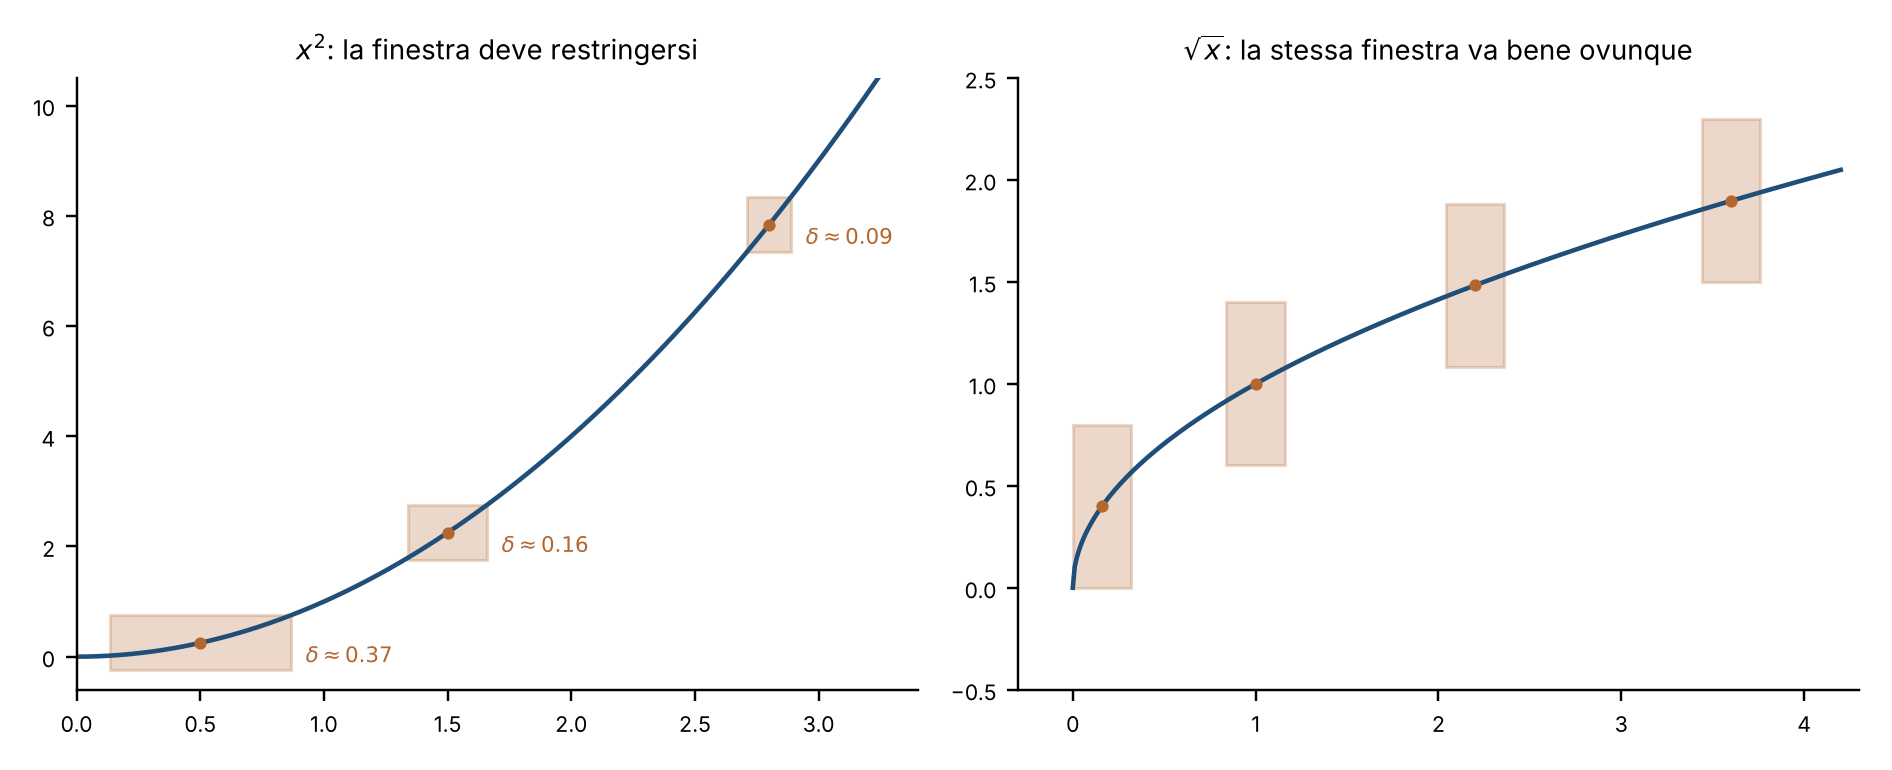
\includegraphics[width=\textwidth]{figure/uniforme.png}
\caption{A sinistra, $f(x)=x^{2}$ con $\epsilon=0{,}5$: per mantenere le variazioni di
$f$ entro $\pm\epsilon$, la finestra deve restringersi man mano che il grafico diventa
più ripido, e la sua semiampiezza è la \eqref{eq:delta-x2}. A destra,
$f(x)=\sqrt x$ con $\epsilon=0{,}4$: la stessa finestra, di semiampiezza
$\delta=\epsilon^{2}=0{,}16$, va bene ovunque, anche vicino all'origine dove la tangente è
verticale (\texttt{python/fig\_uniforme.py}).}
\label{fig:uniforme}
\end{figure}

È opportuno introdurre la definizione seguente.

\begin{definizione}[Funzione uniformemente continua]\label{def:uniformemente-continua}
\index{funzione!uniformemente continua}\index{uniforme continuità}
Si dice che $f:I\to\R$ è \emph{uniformemente continua} nell'intervallo $I$ se per ogni
$\epsilon>0$ esiste $\delta=\delta(\epsilon)>0$ tale che, per ogni $x,x'\in I$,
\begin{equation}\label{eq:uniforme-continuita}
  \abs{x-x'}<\delta \ \implica\ \abs{f(x)-f(x')}<\epsilon .
\end{equation}
\end{definizione}

La differenza con la continuità sta tutta nell'\emph{ordine dei quantificatori}.
Indicata con (C) la condizione
$\abs{x-x_{0}}<\delta\implica\abs{f(x)-f(x_{0})}<\epsilon$, si ha
\[
  \begin{aligned}
    &\text{continuità in } I: &&\perogni x_{0}\in I\ \ \perogni\epsilon>0\ \
    \esiste\delta>0\ \ \perogni x\in I : \ \text{(C)};\\
    &\text{uniforme continuità}: &&\perogni\epsilon>0\ \ \esiste\delta>0\ \
    \perogni x_{0}\in I\ \ \perogni x\in I : \ \text{(C)} .
  \end{aligned}
\]
Nella seconda riga $\delta$ viene scelto \emph{prima} del punto, e deve quindi andar bene
per tutti i punti. Una funzione uniformemente continua è ovviamente continua; il
viceversa è falso, come mostra l'\cref{es:x2-non-uniforme}. Geometricamente, $f$ è
uniformemente continua se un rettangolo di dimensioni fisse $2\delta\times2\epsilon$, fatto
scorrere con il centro sul grafico, è sempre attraversato dal grafico soltanto attraverso
i lati verticali (\cref{fig:uniforme}).

\begin{python}[Il $\delta$ massimo per $x^{2}$ e per $\sqrt x$]
import math

eps = 0.1
print("f(x) = x^2: delta massimo in x0, eps = 0.1")
for x0 in (0, 1, 10, 100, 1000):
    d = math.sqrt(x0**2 + eps) - x0            # formula (delta-x2)
    print(f"   x0 = {x0:7.2f}:  delta = {d:.3e}")
print("f(x) = sqrt(x): delta massimo in x0, eps = 0.1")
for x0 in (0, 0.0025, 1, 100, 1000):
    r = math.sqrt(x0)
    # a destra: (r + eps)^2 - x0;  a sinistra: x0 - (r - eps)^2
    d = 2 * eps * r + eps**2 if r < eps else 2 * eps * r - eps**2
    print(f"   x0 = {x0:7.4g}:  delta = {d:.3e}")
\end{python}
\begin{risultato}
f(x) = x^2: delta massimo in x0, eps = 0.1
   x0 =    0.00:  delta = 3.162e-01
   x0 =    1.00:  delta = 4.881e-02
   x0 =   10.00:  delta = 4.999e-03
   x0 =  100.00:  delta = 5.000e-04
   x0 = 1000.00:  delta = 5.000e-05
f(x) = sqrt(x): delta massimo in x0, eps = 0.1
   x0 =       0:  delta = 1.000e-02
   x0 =  0.0025:  delta = 2.000e-02
   x0 =       1:  delta = 1.900e-01
   x0 =     100:  delta = 1.990e+00
   x0 =    1000:  delta = 6.315e+00
\end{risultato}

Per $x^{2}$ il $\delta$ massimo decresce come $\frac\epsilon{2x_{0}}$; per $\sqrt x$, al
contrario, il più piccolo dei $\delta$ massimi è $\epsilon^{2}>0$ (lo si ha, ad esempio,
nell'origine):
come vedremo nell'\cref{es:radice-uniforme}, la radice quadrata è uniformemente continua
su tutta la semiretta $[0,+\infty)$.

\subsection{Il teorema di Cantor}

Riprendendo l'esempio di $x^{2}$: la funzione non è uniformemente continua su $\R$, ma lo
è in ogni intervallo chiuso e limitato $[a,b]$, grazie al teorema seguente.

\begin{teorema}[di Cantor]\label{teo:cantor}\index{teorema!di Cantor}
Sia $f$ una funzione continua nell'intervallo chiuso e limitato $[a,b]$. Allora $f$ è
uniformemente continua in $[a,b]$.
\end{teorema}

\begin{schema}
\Ipotesi{$f$ continua in $[a,b]$ (chiuso e limitato).}
\Tesi{$\perogni\epsilon>0\ \esiste\delta>0$ : $x,x'\in[a,b]$, $\abs{x-x'}<\delta\implica
\abs{f(x)-f(x')}<\epsilon$.}
\end{schema}

\begin{strategia}
Procediamo per assurdo. Se $f$ non è uniformemente continua, per un certo $\epsilon_{0}$
nessun $\delta$ funziona: scegliendo $\delta=\frac1n$ troviamo coppie di punti
$x_{n}$, $x_{n}'$ sempre più vicine, sulle quali però $f$ differisce di almeno
$\epsilon_{0}$. Qui entra in gioco l'ipotesi che l'intervallo sia chiuso e limitato:
per il teorema di Bolzano--Weierstrass i punti $x_{n}$ hanno un'estratta convergente a
un punto $x_{0}$ di $[a,b]$, e le $x_{n}'$ corrispondenti, vicinissime alle $x_{n}$,
convergono allo stesso punto. La continuità di $f$ in $x_{0}$ costringe allora
$f(x_{n})-f(x_{n}')$ a tendere a zero, in contraddizione con la scelta delle coppie.
\end{strategia}

\begin{dimostrazione}
Procediamo per assurdo. La definizione di uniforme continuità in $[a,b]$ si scrive
\[
  \perogni\epsilon>0\ \ \esiste\delta>0\ \ \perogni x,x'\in[a,b] : \
  \abs{x-x'}<\delta\implica\abs{f(x)-f(x')}<\epsilon ;
\]
la sua negazione afferma che esiste $\epsilon_{0}>0$ tale che, qualunque sia $\delta>0$,
esistono $x,x'\in[a,b]$ (dipendenti da $\delta$) con
\begin{equation}\label{eq:negazione-uc}
  \abs{x-x'}<\delta, \qquad \abs{f(x)-f(x')}\ge\epsilon_{0} .
\end{equation}
Scegliamo $\delta=\frac1n$, con $n\in\N$, e indichiamo con $x_{n}$, $x_{n}'$ i
corrispondenti punti di $[a,b]$ per cui vale la \eqref{eq:negazione-uc}:
\[
  \abs{x_{n}-x_{n}'}<\frac1n, \qquad \abs{f(x_{n})-f(x_{n}')}\ge\epsilon_{0}
  \qquad\perogni n\in\N .
\]
La successione $x_{n}$ è limitata, perché $a\le x_{n}\le b$; per il teorema di
Bolzano--Weierstrass (\cref{teo:bolzano-weierstrass}) esiste un'estratta $x_{n_{k}}$
convergente a un punto $x_{0}$; poiché $a\le x_{n_{k}}\le b$ per ogni $k$, per il
confronto dei limiti (\cref{cor:confronto-limiti}) anche $a\le x_{0}\le b$. È qui che
serve la \emph{chiusura} dell'intervallo. Inoltre
\[
  x_{n_{k}}-\frac1{n_{k}}<x_{n_{k}}'<x_{n_{k}}+\frac1{n_{k}} \qquad\perogni k\in\N,
\]
e poiché $n_{k}\ge k$ (\cref{lem:nk-maggiore-k}) si ha $\frac1{n_{k}}\to0$: per il teorema
dei carabinieri anche $x_{n_{k}}'\to x_{0}$. Le successioni $x_{n_{k}}$ e $x_{n_{k}}'$
sono formate da punti di $[a,b]$ e convergono a $x_{0}\in[a,b]$; per la continuità di
$f$ in $x_{0}$, nella forma (b) della \cref{prop:caratt-continuita},
\[
  \lim_{k\to+\infty}\bigl[f(x_{n_{k}})-f(x_{n_{k}}')\bigr]=f(x_{0})-f(x_{0})=0 ,
\]
in contrasto con il fatto che $\abs{f(x_{n_{k}})-f(x_{n_{k}}')}\ge\epsilon_{0}$ per ogni
$k$. La contraddizione prova la tesi.
\end{dimostrazione}

Entrambe le ipotesi sull'intervallo sono necessarie. Sulla semiretta $[0,+\infty)$,
che è chiusa ma non limitata, $x^{2}$ è continua ma non uniformemente continua
(\cref{es:x2-non-uniforme}); nell'intervallo $(0,1]$, che è limitato ma non chiuso, la
funzione $\frac1x$ è continua ma non uniformemente continua
(\cref{es:uno-su-x-non-uniforme}). In entrambi i casi la dimostrazione si inceppa nello
stesso punto: nel primo la successione $x_{n}$ può non essere limitata, e allora
un'estratta convergente può mancare; nel secondo l'estratta può convergere al punto
$0$, che non appartiene al dominio.

\subsection{Funzioni lipschitziane}

A conclusione del paragrafo riprendiamo una notevole classe di funzioni uniformemente
continue, già incontrata nel \cref{cap:applicazioni-derivate}.

\begin{definizione}[Funzione lipschitziana]\label{def:lipschitziana}
\index{funzione!lipschitziana}
Si dice che $f$ è \emph{lipschitziana} nell'intervallo $I$ se esiste una costante
$L\ge0$, detta \emph{costante di Lipschitz}, tale che
\begin{equation}\label{eq:lipschitziana}
  \abs{f(x)-f(x')}\le L\,\abs{x-x'} \qquad\perogni x,x'\in I .
\end{equation}
\end{definizione}

Per $x\neq x'$ la \eqref{eq:lipschitziana} afferma che le pendenze di tutte le
secanti al grafico sono comprese tra $-L$ e $L$: in ogni punto $(x',f(x'))$ il grafico è
contenuto nel «doppio cono» delimitato dalle rette di pendenza $\pm L$ passanti per quel
punto (\cref{fig:lipschitz}).

\begin{proposizione}[Le lipschitziane sono uniformemente continue]
\label{prop:lipschitz-uniforme}
Una funzione lipschitziana in un intervallo $I$ è uniformemente continua in $I$.
\end{proposizione}

\begin{schema}
\Ipotesi{$\abs{f(x)-f(x')}\le L\abs{x-x'}$ per ogni $x,x'\in I$.}
\Tesi{$f$ uniformemente continua in $I$.}
\end{schema}

\begin{strategia}
La \eqref{eq:lipschitziana} fornisce un $\delta$ esplicito, uguale per tutti i punti:
basta $\delta=\frac\epsilon L$.
\end{strategia}

\begin{dimostrazione}
Se $L=0$, $f$ è costante e la tesi è ovvia. Se $L>0$, fissato $\epsilon>0$ poniamo
$\delta=\frac\epsilon L$: per ogni coppia $x,x'\in I$ con $\abs{x-x'}<\delta$ si ha
$\abs{f(x)-f(x')}\le L\abs{x-x'}<L\delta=\epsilon$.
\end{dimostrazione}

Per le funzioni derivabili la lipschitzianità si legge sulla derivata.

\begin{teorema}[Funzioni derivabili e lipschitziane]\label{teo:lipschitz-derivata}
Sia $f$ derivabile nell'intervallo $I$. Allora $f$ è lipschitziana in $I$ con costante
$L$ se e solo se $\abs{f'(x)}\le L$ per ogni $x\in I$.
\end{teorema}

\begin{schema}
\Ipotesi{$f$ derivabile nell'intervallo $I$; \ $L\ge0$.}
\Tesi{$\abs{f(x)-f(x')}\le L\abs{x-x'}\ \perogni x,x'\in I \ \sse\ \abs{f'}\le L$ in $I$.}
\end{schema}

\begin{strategia}
Una implicazione è il corollario del teorema di Lagrange già dimostrato nel
\cref{cap:applicazioni-derivate}. Per l'altra, la \eqref{eq:lipschitziana} dice che i
rapporti incrementali sono in valore assoluto al più $L$, e il confronto dei limiti
trasmette la stima alla derivata.
\end{strategia}

\begin{dimostrazione}
Se $\abs{f'(x)}\le L$ per ogni $x\in I$, la \eqref{eq:lipschitziana} è la tesi del
\cref{cor:lipschitz}, conseguenza del teorema di Lagrange. Viceversa, sia $f$
lipschitziana con costante $L$ e sia $x\in I$. Per $h\neq0$ con $x+h\in I$ si ha
\[
  \biggl|\frac{f(x+h)-f(x)}h\biggr|\le L .
\]
Per $h\to0$ il rapporto incrementale tende a $f'(x)$, e il suo valore assoluto a
$\abs{f'(x)}$ (per la continuità del valore assoluto); per il confronto dei limiti
(\cref{teo:confronto-funzioni}(ii)) si ottiene $\abs{f'(x)}\le L$.
\end{dimostrazione}

\begin{esempio}[Tre funzioni a confronto]\label{es:lipschitz-esempi}
Tre esempi mostrano i legami tra derivabilità, lipschitzianità e uniforme continuità.
\begin{enumerate}[label=\textup{(\alph*)}]
  \item $\sen x$ è lipschitziana in $\R$ con costante $1$, perché
  $\abs{D\sen x}=\abs{\cos x}\le1$ per ogni $x$; la stessa disuguaglianza
  $\abs{\sen x-\sen x'}\le\abs{x-x'}$ era stata ottenuta nell'\cref{es:seno-lipschitz}
  con le formule di prostaferesi e la disuguaglianza $\abs{\sen t}\le\abs t$.
  \item $\abs x$ è lipschitziana in $\R$ con costante $1$, per la disuguaglianza
  triangolare inversa \eqref{eq:modulo-lipschitz}, ma non è derivabile in $0$: il
  \cref{teo:lipschitz-derivata} non si applica, e una funzione lipschitziana non è
  necessariamente derivabile.
  \item $\sqrt x$ è uniformemente continua in $[0,1]$ per il teorema di Cantor, ma non è
  lipschitziana: la pendenza della secante tra $0$ e $x$ è
  $\frac{\sqrt x-0}{x-0}=\frac1{\sqrt x}$, che tende a $+\infty$ per $x\to0^{+}$, mentre
  dovrebbe essere al più $L$. Equivalentemente, per il \cref{teo:lipschitz-derivata}
  applicato in $(0,1]$, la derivata $\frac1{2\sqrt x}$ non è limitata.
\end{enumerate}
\end{esempio}

\begin{figure}[htb]
\centering
\begin{tikzpicture}
\begin{axis}[name=l1, width=0.55\textwidth, height=4.6cm, axis lines=middle, axis on top,
  xmin=-0.3, xmax=6.5, ymin=-1.9, ymax=2.4, xtick=\empty, ytick=\empty,
  title={\scriptsize $\sen x$: il doppio cono di pendenza $\pm1$}]
  \fill[verde!15] (axis cs:2,0.909) -- (axis cs:6.3,5.209) -- (axis cs:6.3,-3.391)
    -- cycle;
  \fill[verde!15] (axis cs:2,0.909) -- (axis cs:-0.3,3.209) -- (axis cs:-0.3,-1.391)
    -- cycle;
  \addplot[verde!60!black, domain=-0.3:6.3] {0.909+(x-2)};
  \addplot[verde!60!black, domain=-0.3:6.3] {0.909-(x-2)};
  \addplot[curva, domain=-0.3:6.3, samples=120] {sin(deg(x))};
  \addplot[only marks, mark=*, mark size=1.6pt, rame] coordinates {(2,0.909)};
\end{axis}
\begin{axis}[at={(l1.east)}, anchor=west, xshift=0.7cm, width=0.5\textwidth,
  height=4.6cm, axis lines=middle, xmin=-0.05, xmax=1.1, ymin=-0.05, ymax=1.15,
  xtick=\empty, ytick=\empty, title={\scriptsize $\sqrt x$: secanti sempre più ripide}]
  \addplot[curva, domain=0:1.05, samples=200] {sqrt(x)};
  \addplot[rame, domain=0:1.05] {x};
  \addplot[rame, domain=0:0.3] {2*x};
  \addplot[rame, domain=0:0.12] {5*x};
  \addplot[rame, domain=0:0.055] {12*x};
  \addplot[only marks, mark=*, mark size=1.2pt, rame] coordinates
    {(1,1) (0.25,0.5) (0.04,0.2) (0.00694,0.0833)};
  \node[font=\scriptsize, rame, anchor=west] at (axis cs:0.9,0.82) {$1$};
  \node[font=\scriptsize, rame, anchor=west] at (axis cs:0.28,0.62) {$2$};
  \node[font=\scriptsize, rame, anchor=west] at (axis cs:0.11,0.62) {$5$};
  \node[font=\scriptsize, rame, anchor=south] at (axis cs:0.052,0.66) {$12$};
\end{axis}
\end{tikzpicture}
\caption{A sinistra, una funzione lipschitziana con costante $L=1$: il grafico di
$\sen x$ resta nel doppio cono verde, delimitato dalle rette di pendenza $\pm1$ per il
punto evidenziato, e così per ogni altro punto. A destra, le secanti al grafico di
$\sqrt x$ uscenti dall'origine hanno pendenze $1$, $2$, $5$, $12$, \dots, non limitate:
nessun cono di apertura finita contiene il grafico vicino all'origine.}
\label{fig:lipschitz}
\end{figure}

\begin{esempio}[La radice quadrata è uniformemente continua su $\lbrack0,+\infty)$]
\label{es:radice-uniforme}
Il teorema di Cantor non si applica alla semiretta, ma per la radice quadrata vale una
stima diretta: per $0\le x'\le x$,
\begin{equation}\label{eq:radice-holder}
  \sqrt x-\sqrt{x'}\le\sqrt{x-x'} .
\end{equation}
Infatti, elevando al quadrato i due membri non negativi di
$\sqrt x\le\sqrt{x-x'}+\sqrt{x'}$, la disuguaglianza equivale a
$x\le(x-x')+2\sqrt{x'(x-x')}+x'$, cioè a $0\le2\sqrt{x'(x-x')}$, che è vera. Dunque
$\abs{\sqrt x-\sqrt{x'}}\le\sqrt{\abs{x-x'}}$ per ogni $x,x'\ge0$, e posto
$\delta=\epsilon^{2}$ si ha $\abs{\sqrt x-\sqrt{x'}}<\epsilon$ non appena
$\abs{x-x'}<\delta$: la radice è uniformemente continua in $[0,+\infty)$ pur non essendo
lipschitziana. Una stima del tipo $\abs{f(x)-f(x')}\le L\abs{x-x'}^{\alpha}$, con
$0<\alpha\le1$, si chiama \emph{condizione di Hölder}; per $\alpha=1$ è la
lipschitzianità.
\end{esempio}

\begin{python}[Pendenze delle secanti: seno e radice quadrata]
import math, random

random.seed(1)
pend = []
for _ in range(100000):
    x, y = random.uniform(-10, 10), random.uniform(-10, 10)
    if x != y:
        pend.append(abs(math.sin(x) - math.sin(y)) / abs(x - y))
print(f"sen x: pendenza massima delle secanti = {max(pend):.6f}")
for h in (1e-2, 1e-4, 1e-6, 1e-8):
    print(f"sqrt(x): pendenza della secante tra 0 e {h:.0e}"
          f" = {math.sqrt(h) / h:7.0f}")
\end{python}
\begin{risultato}
sen x: pendenza massima delle secanti = 0.999970
sqrt(x): pendenza della secante tra 0 e 1e-02 =      10
sqrt(x): pendenza della secante tra 0 e 1e-04 =     100
sqrt(x): pendenza della secante tra 0 e 1e-06 =    1000
sqrt(x): pendenza della secante tra 0 e 1e-08 =   10000
\end{risultato}

Riassumendo, per una funzione definita in un intervallo valgono le implicazioni
illustrate nella \cref{fig:gerarchia}, nessuna delle quali si può invertire.

\begin{figure}[htb]
\centering
\begin{tikzpicture}[box/.style={draw=blu, fill=blu!8, rounded corners=2pt,
  font=\scriptsize, align=center, inner sep=4pt, minimum height=1.0cm,
  text width=1.95cm}]
  \node[box] (a) at (0,0) {derivabile con\\ $f'$ limitata};
  \node[box] (b) at (2.85,0) {lipschitziana};
  \node[box] (c) at (5.7,0) {uniformemente\\ continua};
  \node[box] (d) at (8.55,0) {continua};
  \draw[-Latex, thick, grigio] (a) -- (b);
  \draw[-Latex, thick, grigio] (b) -- (c);
  \draw[-Latex, thick, grigio] (c) -- (d);
  \node[font=\scriptsize, rame, align=center] at (1.425,-1.0) {$\abs x$ su $\R$};
  \node[font=\scriptsize, rame, align=center] at (4.275,-1.0) {$\sqrt x$ su $[0,1]$};
  \node[font=\scriptsize, rame, align=center] at (7.125,-1.05)
    {$x^{2}$ su $\R$,\\ $\frac1x$ su $(0,1]$};
\end{tikzpicture}
\caption{Le implicazioni tra le classi di funzioni in un intervallo. Sotto ciascuna
freccia, una funzione che appartiene alla classe di destra ma non a quella di sinistra.
Per un intervallo chiuso e limitato, il teorema di Cantor rende equivalenti le ultime
due classi.}
\label{fig:gerarchia}
\end{figure}

\begin{notastorica}[Dirichlet, Heine, Cantor]
Nella dimostrazione dell'integrabilità delle funzioni continue data da Cauchy nel 1823
c'era una lacuna: Cauchy usava senza accorgersene la continuità \emph{uniforme}, non
distinguendola da quella puntuale. La distinzione maturò negli anni successivi.
Peter Gustav Lejeune Dirichlet dimostrò il teorema che abbiamo chiamato di Cantor nelle
sue lezioni berlinesi del 1854 sugli integrali definiti, pubblicate però soltanto nel
1904. Il primo a pubblicare questi risultati fu Eduard Heine: la definizione di
uniforme continuità nel 1870, il teorema nel 1872, in un articolo sui fondamenti della
teoria delle funzioni nel quale riconosceva il proprio debito verso le idee di
Weierstrass e di Georg Cantor; per questo il teorema è noto anche come teorema di
Heine--Cantor. Rudolf Lipschitz considerò per la prima volta una condizione del tipo
\eqref{eq:lipschitziana} nel 1864, studiando la convergenza delle serie di Fourier; nel
1876 la pose come ipotesi che garantisce l'esistenza e l'unicità delle soluzioni delle
equazioni differenziali. È ancora oggi l'ipotesi standard dei teoremi di esistenza e
unicità che si incontrano, ad esempio, nello studio della dinamica del volo.
\end{notastorica}

%% ----------------------------------------------------------------------------
%%  §8.6  Appendice: integrabilità delle funzioni continue e monotòne
%% ----------------------------------------------------------------------------
\section{Appendice: integrabilità delle funzioni continue e monotòne}
\label{sec:integrabilita-continue}

Possiamo ora dimostrare il risultato che rende la teoria dell'integrale utilizzabile in
pratica: tutte le funzioni continue in un intervallo chiuso e limitato sono
integrabili. Lo otterremo in una forma più forte, che riguarda \emph{tutte} le
partizioni di ampiezza sufficientemente piccola, e che giustificherà le formule di
quadratura numerica.

\begin{teorema}[Integrabilità delle funzioni continue]\label{teo:integrabilita-continue}
\index{funzione!continua!integrabilità}
Sia $f$ una funzione continua in $[a,b]$. Allora $f$ è integrabile secondo Riemann in
$[a,b]$. Più precisamente, per ogni $\epsilon>0$ esiste $\delta>0$ tale che
\begin{equation}\label{eq:ampiezza-piccola}
  \abs P<\delta \ \implica\ S(P)-s(P)<\epsilon \qquad\text{per ogni partizione $P$ di }
  [a,b] .
\end{equation}
\end{teorema}

\begin{schema}
\Ipotesi{$f$ continua in $[a,b]$, $a<b$.}
\Tesi{$f$ integrabile in $[a,b]$; \ $\perogni\epsilon>0\ \esiste\delta>0$ :
$\abs P<\delta\implica S(P)-s(P)<\epsilon$.}
\end{schema}

\begin{strategia}
Per la \eqref{eq:S-s-oscillazioni} basta rendere tutte le oscillazioni $M_{k}-m_{k}$
minori di $\frac\epsilon{b-a}$: allora $S(P)-s(P)<\frac\epsilon{b-a}\sum\Delta
x_{k}=\epsilon$. Il teorema di Weierstrass assicura che $m_{k}$ e $M_{k}$ sono valori di
$f$ in due punti dell'intervallo $[x_{k-1},x_{k}]$, la cui distanza non supera
l'ampiezza della partizione; il teorema di Cantor fornisce un $\delta$, \emph{uguale per
tutti gli intervalli}, che rende piccola la differenza tra due valori di $f$ in punti
distanti meno di $\delta$.
\end{strategia}

\begin{dimostrazione}
La funzione $f$ è limitata per il teorema di Weierstrass, quindi le somme integrali
sono definite. Fissato $\epsilon>0$, per il teorema di Cantor (\cref{teo:cantor}) $f$ è
uniformemente continua in $[a,b]$, ed esiste $\delta>0$ tale che
\begin{equation}\label{eq:cantor-integrabilita}
  \abs{f(x)-f(x')}<\frac\epsilon{b-a} \qquad\text{per ogni } x,x'\in[a,b] \text{ con }
  \abs{x-x'}<\delta .
\end{equation}
Sia $P=\set{x_{0},\dots,x_{n}}$ una partizione con $\abs P<\delta$. In ogni intervallo
$[x_{k-1},x_{k}]$ la funzione continua $f$ assume minimo e massimo (\cref{teo:weierstrass}):
esistono $\xi_{k},\eta_{k}\in[x_{k-1},x_{k}]$ con $m_{k}=f(\xi_{k})$ e $M_{k}=f(\eta_{k})$.
Poiché $\abs{\xi_{k}-\eta_{k}}\le\Delta x_{k}\le\abs P<\delta$, per la
\eqref{eq:cantor-integrabilita}
\[
  M_{k}-m_{k}=f(\eta_{k})-f(\xi_{k})<\frac\epsilon{b-a} \qquad\perogni k=1,\dots,n ,
\]
e quindi
\[
  S(P)-s(P)=\sum_{k=1}^{n}(M_{k}-m_{k})\,\Delta x_{k}
  <\frac\epsilon{b-a}\sum_{k=1}^{n}\Delta x_{k}=\epsilon .
\]
Questo prova la \eqref{eq:ampiezza-piccola}. Partizioni di ampiezza minore di $\delta$
esistono (ad esempio la partizione uniforme in $n$ parti, con $n>\frac{b-a}\delta$), e il
criterio di integrabilità (\cref{teo:criterio-integrabilita}) dà l'integrabilità di
$f$.
\end{dimostrazione}

La forma forte \eqref{eq:ampiezza-piccola} ha una conseguenza importante: per una
funzione continua, l'integrale è il limite di \emph{qualsiasi} successione di somme di
Riemann, purché l'ampiezza delle partizioni tenda a zero.

\begin{teorema}[Convergenza delle somme di Riemann]\label{teo:riemann-continue}
Sia $f$ continua in $[a,b]$, sia $P_{n}$ una successione di partizioni di $[a,b]$ con
$\abs{P_{n}}\to0$, e sia $\sigma_{n}$ una somma di Riemann \eqref{eq:somma-riemann}
relativa a $P_{n}$, con punti $\xi_{k}$ scelti in modo arbitrario. Allora
\begin{equation}\label{eq:riemann-limite}
  \lim_{n\to+\infty}\sigma_{n}=\int_{a}^{b}f(x)\,dx .
\end{equation}
\end{teorema}

\begin{schema}
\Ipotesi{$f$ continua in $[a,b]$; \ $\abs{P_{n}}\to0$; \ $\sigma_{n}$ somma di Riemann
relativa a $P_{n}$.}
\Tesi{$\sigma_{n}\to\int_{a}^{b}f$.}
\end{schema}

\begin{strategia}
Ogni somma di Riemann dista dall'integrale al più $S(P)-s(P)$ \eqref{eq:riemann-stima}, e
questa quantità è piccola quando l'ampiezza della partizione è piccola, per la
\eqref{eq:ampiezza-piccola}.
\end{strategia}

\begin{dimostrazione}
Sia $\epsilon>0$ e sia $\delta$ quello del \cref{teo:integrabilita-continue}. Poiché
$\abs{P_{n}}\to0$, esiste $\nu$ tale che $\abs{P_{n}}<\delta$ per ogni $n>\nu$; per tali $n$,
la \eqref{eq:riemann-stima} e la \eqref{eq:ampiezza-piccola} danno
$\bigl|\sigma_{n}-\int_{a}^{b}f\bigr|\le S(P_{n})-s(P_{n})<\epsilon$.
\end{dimostrazione}

In particolare, per $f$ continua le medie aritmetiche di $n$ campioni equispaziati,
come quelle considerate all'inizio del \cref{sec:media}, tendono alla media integrale.

\subsection{Funzioni monotòne}

La continuità è sufficiente ma non necessaria per l'integrabilità: la funzione
dell'\cref{oss:media-discontinua} è discontinua ma integrabile. Un'altra classe
importante di funzioni integrabili, che comprende funzioni discontinue, è quella delle
funzioni monotòne.

\begin{teorema}[Integrabilità delle funzioni monotòne]\label{teo:integrabilita-monotone}
\index{funzione!monotòna!integrabilità}
Sia $f$ monotòna in $[a,b]$. Allora $f$ è integrabile secondo Riemann in $[a,b]$, e per
la partizione uniforme $P_{n}$ in $n$ parti risulta
\begin{equation}\label{eq:monotone-S-s}
  S(P_{n})-s(P_{n})=\frac{\abs{f(b)-f(a)}\,(b-a)}n .
\end{equation}
\end{teorema}

\begin{schema}
\Ipotesi{$f$ monotòna in $[a,b]$.}
\Tesi{$f$ integrabile; \ $S(P_{n})-s(P_{n})=\abs{f(b)-f(a)}\frac{b-a}n$.}
\end{schema}

\begin{strategia}
È il calcolo già fatto per $x^{2}$, per la distribuzione ellittica e per
$e^{-x^{2}}$: in ogni intervallo gli estremi di una funzione monotòna sono i valori negli
estremi dell'intervallo, e la differenza tra le somme è telescopica.
\end{strategia}

\begin{dimostrazione}
Una funzione monotòna in $[a,b]$ è limitata, perché i suoi valori sono compresi tra
$f(a)$ e $f(b)$. Sia $f$ crescente e sia $x_{k}=a+k\frac{b-a}n$. Per
$x\in[x_{k-1},x_{k}]$ si ha $f(x_{k-1})\le f(x)\le f(x_{k})$, e i valori $f(x_{k-1})$,
$f(x_{k})$ sono assunti; quindi $m_{k}=f(x_{k-1})$ e $M_{k}=f(x_{k})$, e
\[
  S(P_{n})-s(P_{n})=\frac{b-a}n\sum_{k=1}^{n}\bigl[f(x_{k})-f(x_{k-1})\bigr]
  =\frac{b-a}n\bigl[f(b)-f(a)\bigr] .
\]
Se $f$ è decrescente, si scambiano i ruoli di $x_{k-1}$ e $x_{k}$ e si ottiene
$\frac{b-a}n\bigl[f(a)-f(b)\bigr]$. In entrambi i casi vale la \eqref{eq:monotone-S-s}, che
tende a zero, e il \cref{cor:limite-somme} dà l'integrabilità.
\end{dimostrazione}

Una funzione monotòna può avere infiniti punti di discontinuità (che sono salti, per il
\cref{cor:monotone-salti}). Ad esempio, la funzione definita in $[0,1]$ da $f(0)=0$ e
$f(x)=\frac1n$ per $\frac1{n+1}<x\le\frac1n$, $n\in\N$, è crescente, ha un salto in ciascuno
dei punti $\frac1n$ con $n\ge2$, ed è integrabile per il \cref{teo:integrabilita-monotone}.

\subsection{Formule di quadratura}

Il \cref{teo:riemann-continue} giustifica il calcolo numerico degli integrali delle
funzioni continue mediante somme di Riemann. Con la partizione uniforme di passo
$h=\frac{b-a}n$ e nodi $x_{k}=a+kh$, le formule più semplici sono quella dei
\emph{rettangoli} (con l'estremo sinistro), quella del \emph{punto medio} e quella dei
\emph{trapezi}:
\begin{align}
  R_{n}&=h\sum_{k=0}^{n-1}f(x_{k}),
  \label{eq:quadratura-rettangoli}\\
  M_{n}&=h\sum_{k=1}^{n}f\Bigl(\frac{x_{k-1}+x_{k}}2\Bigr),
  \label{eq:quadratura-medio}\\
  T_{n}&=h\Bigl[\frac{f(x_{0})+f(x_{n})}2+\sum_{k=1}^{n-1}f(x_{k})\Bigr].
  \label{eq:quadratura-trapezi}
\end{align}
Le prime due sono somme di Riemann, e convergono all'integrale per il
\cref{teo:riemann-continue}. La terza è la media aritmetica della somma dei rettangoli
con l'estremo sinistro e di quella con l'estremo destro, e converge per lo stesso
motivo; il nome deriva dal fatto che, per $f\ge0$, $T_{n}$ è la somma delle aree dei
trapezi di altezza $h$ e basi $f(x_{k-1})$, $f(x_{k})$ (\cref{fig:quadratura}).

Le tre formule non convergono però con la stessa rapidità. Per una funzione monotòna
l'errore della formula dei rettangoli non supera la \eqref{eq:monotone-S-s}, che è
dell'ordine di $\frac1n$, e in generale non è più piccolo. Per il punto medio e per i
trapezi, invece, si dimostra con la formula di Taylor (lo si fa nei corsi di Calcolo
numerico) che, se $f$ ha derivata seconda continua,
\begin{equation}\label{eq:errori-quadratura}
\begin{aligned}
  \Bigl|M_{n}-\int_{a}^{b}f\Bigr|&\le\frac{(b-a)\,h^{2}}{24}\max_{[a,b]}\abs{f''},\\
  \Bigl|T_{n}-\int_{a}^{b}f\Bigr|&\le\frac{(b-a)\,h^{2}}{12}\max_{[a,b]}\abs{f''} :
\end{aligned}
\end{equation}
raddoppiando $n$ l'errore si riduce di circa quattro volte. Inoltre l'errore del punto
medio è circa la metà di quello dei trapezi e di segno opposto, per cui la combinazione
$\frac{2M_{n}+T_{n}}3$, che è la \emph{formula di Cavalieri--Simpson}, elimina il termine
principale dell'errore. Il programma seguente lo verifica sull'integrale
$\int_{0}^{1}e^{-x^{2}}dx$ dell'\cref{es:stima-gaussiana}.

\begin{python}[Formule di quadratura a confronto]
import math

f = lambda x: math.exp(-x * x)
I = math.erf(1) * math.sqrt(math.pi) / 2     # valore di riferimento

def quadrature(f, a, b, n):
    """Rettangoli, punto medio, trapezi, Cavalieri-Simpson."""
    h = (b - a) / n
    x = [a + k * h for k in range(n + 1)]
    ret = h * sum(f(x[k]) for k in range(n))
    med = h * sum(f(x[k] + h / 2) for k in range(n))
    tra = h * (sum(f(t) for t in x) - (f(a) + f(b)) / 2)
    return ret, med, tra, (2 * med + tra) / 3

print("errori assoluti")
print(f"{'n':>4} {'rettangoli':>11} {'p. medio':>10}"
      f" {'trapezi':>10} {'Simpson':>10}")
for n in (4, 8, 16, 32, 64):
    err = [abs(q - I) for q in quadrature(f, 0, 1, n)]
    print(f"{n:4d} " + " ".join(f"{e:10.2e}" for e in err))
\end{python}
\begin{risultato}
errori assoluti
   n  rettangoli   p. medio    trapezi    Simpson
   4   7.52e-02   1.92e-03   3.84e-03   1.99e-06
   8   3.85e-02   4.79e-04   9.59e-04   1.25e-07
  16   1.95e-02   1.20e-04   2.40e-04   7.79e-09
  32   9.82e-03   2.99e-05   5.99e-05   4.87e-10
  64   4.92e-03   7.48e-06   1.50e-05   3.05e-11
\end{risultato}

\begin{figure}[htb]
\centering
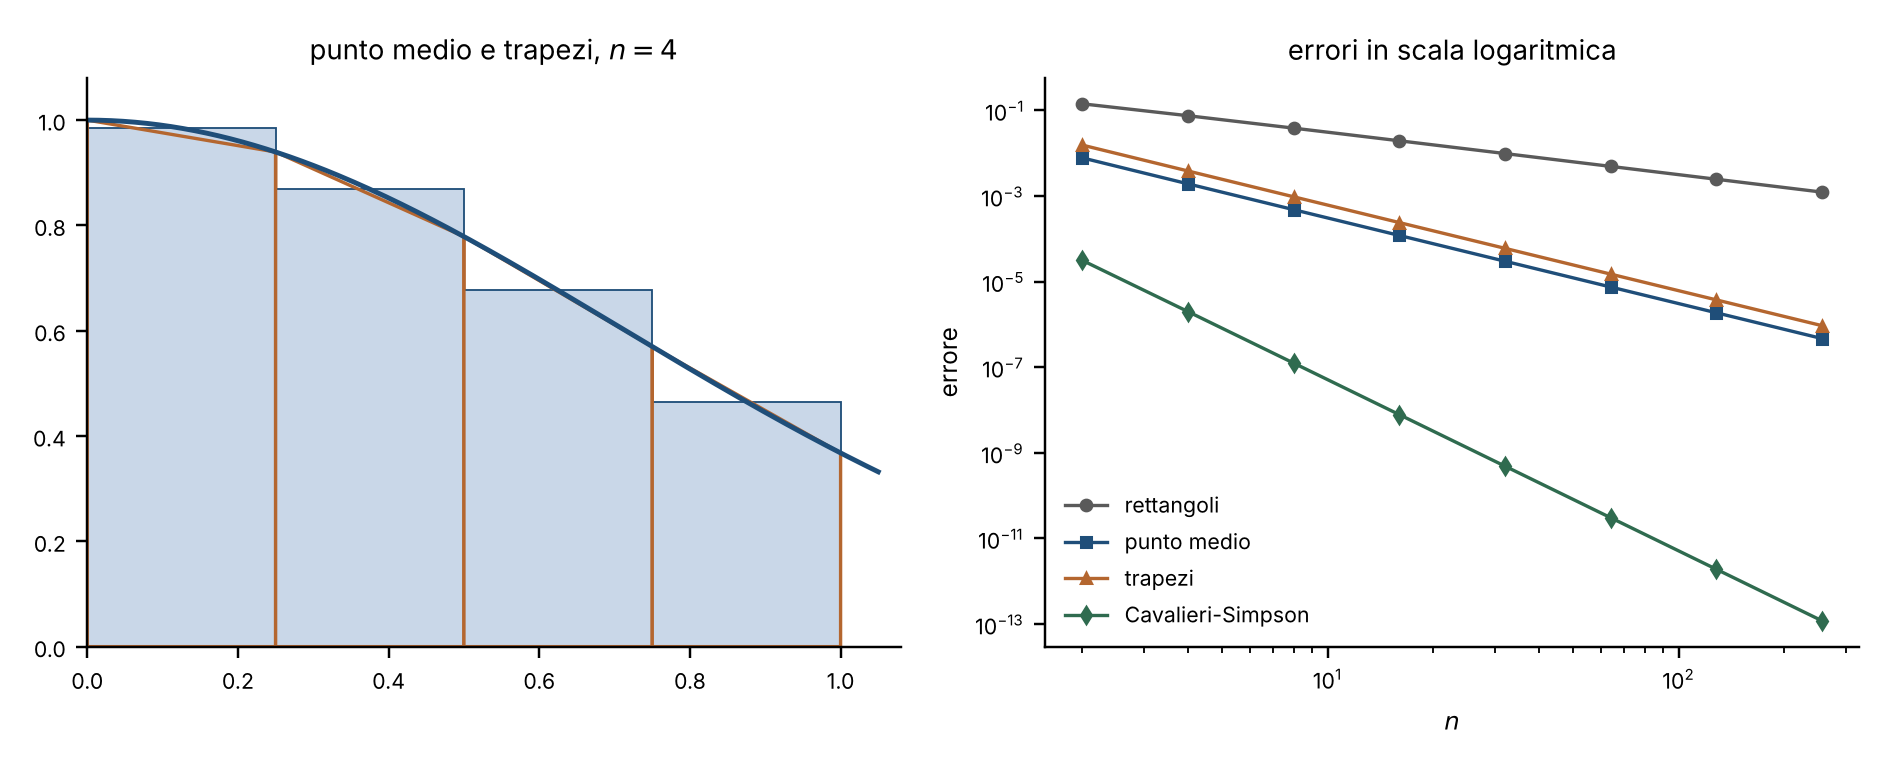
\includegraphics[width=\textwidth]{figure/quadratura.png}
\caption{A sinistra, le formule del punto medio (rettangoli azzurri) e dei trapezi
(contorni in color rame) per $e^{-x^{2}}$ in $[0,1]$ con $n=4$. A destra, gli errori
delle quattro formule in funzione di $n$, in scala logaritmica: le pendenze $-1$, $-2$
e $-4$ corrispondono a errori proporzionali a $\frac1n$, $\frac1{n^{2}}$, $\frac1{n^{4}}$
(\texttt{python/fig\_quadratura.py}).}
\label{fig:quadratura}
\end{figure}

\begin{notastorica}[Da Cauchy a Lebesgue]
Cauchy dimostrò nel 1823 che le somme costruite sugli estremi sinistri di una funzione
continua convergono, quando l'ampiezza della partizione tende a zero, a un limite
indipendente dalle partizioni: è un caso particolare del nostro
\cref{teo:riemann-continue} (sulla lacuna della dimostrazione si veda la nota del
\S\ref{sec:uniforme-continuita}). Riemann, con il suo criterio, estese l'integrale a
funzioni con infinite discontinuità: quali funzioni limitate sono integrabili?
Dirichlet, nella memoria del 1829 in cui compare la sua funzione (\cref{oss:dirichlet}),
aveva indicato come necessario che tra due punti qualsiasi si trovasse sempre un
intervallo di continuità; ma Riemann costruì una funzione integrabile discontinua in un
insieme denso. Hermann Hankel (1870) credette che un insieme non denso in alcun
intervallo si potesse racchiudere in un numero finito di intervalli di lunghezza totale
piccola a piacere; Henry Smith (1875) mostrò che non è così. La risposta
definitiva venne all'inizio del Novecento da Henri Lebesgue e, indipendentemente, da
Giuseppe Vitali (1903): sono integrabili le funzioni limitate il cui insieme dei punti di
discontinuità ha \emph{misura nulla}, cioè si può ricoprire con una successione di
intervalli di lunghezza totale piccola a piacere (come l'insieme numerabile dei salti di
una funzione monotòna, ma non $[0,1]$, dove è discontinua la funzione di Dirichlet).
Quanto alle formule di quadratura, quella che in Italia porta il nome di
Cavalieri--Simpson era nota, in forme equivalenti, a Keplero, che nel 1615 la usò per
stimare il volume delle botti, a Bonaventura Cavalieri e a James Gregory, prima che
Thomas Simpson la diffondesse nel 1743.
\end{notastorica}

%% ----------------------------------------------------------------------------
%%  §8.7  Esercizi di riepilogo
%% ----------------------------------------------------------------------------
\section{Esercizi di riepilogo}
\label{sec:esercizi-cap8}

Come nei capitoli precedenti, ogni soluzione è accompagnata da una nota sulla
\emph{scelta logica} che la guida.

\needspace{8\baselineskip}
\subsection*{Somme integrali e definizione}

\begin{esercizio}\label{es:integrale-x3}
Dimostrare per induzione che $\sum_{k=1}^{n}k^{3}=\bigl(\frac{n(n+1)}2\bigr)^{2}$ e dedurne
che $\int_{0}^{b}x^{3}\,dx=\frac{b^{4}}4$ per ogni $b>0$.
\begin{soluzione}
Per $n=1$ entrambi i membri valgono $1$. Se la formula vale per $n$, allora
$\sum_{k=1}^{n+1}k^{3}=\frac{n^{2}(n+1)^{2}}4+(n+1)^{3}=\frac{(n+1)^{2}}4\bigl(n^{2}+4n+4\bigr)
=\frac{(n+1)^{2}(n+2)^{2}}4$, che è la formula per $n+1$. Per la partizione uniforme di
$[0,b]$ e la funzione crescente $x^{3}$, $M_{k}=x_{k}^{3}$ e $m_{k}=x_{k-1}^{3}$:
\[
  S(P_{n})=\frac bn\sum_{k=1}^{n}\frac{k^{3}b^{3}}{n^{3}}=\frac{b^{4}}4\cdot\frac{(n+1)^{2}}{n^{2}},
  \qquad
  s(P_{n})=\frac{b^{4}}4\cdot\frac{(n-1)^{2}}{n^{2}} ,
\]
con $S(P_{n})-s(P_{n})=\frac{b^{4}}n\to0$ (somma telescopica, come nella
\eqref{eq:monotone-S-s}). Per il \cref{cor:limite-somme} l'integrale è il limite comune,
$\frac{b^{4}}4$. \emph{Scelta logica:} lo schema è quello del settore di parabola; i
risultati $\frac{b^{2}}2$, $\frac{b^{3}}3$, $\frac{b^{4}}4$ suggeriscono
$\int_{0}^{b}x^{p}\,dx=\frac{b^{p+1}}{p+1}$, e la derivata rispetto a $b$ di ciascuno è
$b^{p}$: è ancora l'indizio dell'\cref{oss:indizio-tfc}.
\end{soluzione}
\end{esercizio}

\begin{esercizio}\label{es:integrale-esponenziale}
Calcolare $\int_{0}^{1}2^{x}\,dx$ con le somme integrali relative alla partizione
uniforme.
\begin{soluzione}
La funzione è crescente, quindi $M_{k}=2^{k/n}$. Posto $q=2^{1/n}$, la somma superiore è
una progressione geometrica (\cref{prop:geometrica}):
\[
  S(P_{n})=\frac1n\sum_{k=1}^{n}q^{k}=\frac1n\cdot\frac{q\,(q^{n}-1)}{q-1}
  =2^{1/n}\cdot\frac{1/n}{2^{1/n}-1},
\]
perché $q^{n}=2$. Per il limite notevole \eqref{eq:ln-exp}, calcolato lungo la
successione $\frac1n\to0$, $\frac{2^{1/n}-1}{1/n}\to\log2$; inoltre $2^{1/n}\to1$. Dunque
$S(P_{n})\to\frac1{\log2}$. Per il \cref{teo:integrabilita-monotone},
$S(P_{n})-s(P_{n})=\frac1n(2-1)\to0$, e quindi anche $s(P_{n})\to\frac1{\log2}$: per il
\cref{cor:limite-somme}
$\int_{0}^{1}2^{x}\,dx=\frac1{\log2}\approx1{,}4427$. \emph{Scelta logica:} per gli
esponenziali la partizione uniforme trasforma la somma in una progressione geometrica
(nel procedimento di Fermat la progressione geometrica compariva invece nei nodi della
partizione); il calcolo si chiude con un limite notevole del
\cref{cap:funzioni-continue}.
\end{soluzione}
\end{esercizio}

\begin{esercizio}\label{es:integrale-a-b}
Dimostrare che, per $0\le a<b$, $\int_{a}^{b}x\,dx=\frac{b^{2}-a^{2}}2$ e
$\int_{a}^{b}x^{2}\,dx=\frac{b^{3}-a^{3}}3$, e calcolare la media integrale di $x^{2}$ in
$[a,b]$.
\begin{soluzione}
Per l'additività (\cref{teo:additivita}), $\int_{0}^{b}=\int_{0}^{a}+\int_{a}^{b}$, quindi
$\int_{a}^{b}x^{2}\,dx=\frac{b^{3}}3-\frac{a^{3}}3$ per la \eqref{eq:integrale-x2}, e
analogamente per $x$. La media è
$\frac{b^{3}-a^{3}}{3(b-a)}=\frac{a^{2}+ab+b^{2}}3$. \emph{Scelta logica:} l'additività
permette di ottenere l'integrale su un intervallo qualsiasi da quelli con primo estremo
nell'origine, senza nuove somme.
\end{soluzione}
\end{esercizio}

\begin{esercizio}\label{es:valore-in-un-punto}
Sia $f$ integrabile in $[a,b]$ e sia $g$ una funzione che differisce da $f$ in un solo
punto $\bar x$. Dimostrare che $g$ è integrabile e che $\int_{a}^{b}g=\int_{a}^{b}f$.
\begin{soluzione}
La funzione $h=g-f$ è nulla tranne che in $\bar x$, dove vale $d\neq0$; supponiamo
$d>0$ (altrimenti si ragiona su $-h$). In ogni intervallo di una partizione $P$ esistono
punti diversi da $\bar x$, quindi $m_{k}=0$ e $s(P,h)=0$; inoltre $M_{k}=d$ negli intervalli
(al più due) che contengono $\bar x$, e $M_{k}=0$ negli altri, quindi
$0\le S(P,h)\le2d\abs P$. Per la partizione uniforme $P_{n}$, $S(P_{n},h)-s(P_{n},h)\to0$, e
per il \cref{cor:limite-somme} $h$ è integrabile con integrale $0$. Per la linearità,
$g=f+h$ è integrabile e $\int g=\int f+0$. Ripetendo il ragionamento, la conclusione vale
anche se $g$ differisce da $f$ in un numero finito di punti. \emph{Scelta logica:} un
punto «non ha larghezza», e i rettangoli che lo contengono hanno area totale piccola
quanto l'ampiezza della partizione. Modificando $f$ in \emph{infiniti} punti, invece,
l'integrabilità si può perdere: la funzione di Dirichlet si ottiene dalla funzione
nulla cambiandone il valore nei razionali.
\end{soluzione}
\end{esercizio}

\begin{esercizio}
Sia $f(x)=x$ per $x\in\Q$ e $f(x)=0$ per $x\notin\Q$. Calcolare l'integrale inferiore e
l'integrale superiore di $f$ in $[0,1]$.
\begin{soluzione}
In ogni intervallo $[x_{k-1},x_{k}]$ ci sono irrazionali, dove $f=0$, e razionali
arbitrariamente vicini a $x_{k}$, per la densità di $\Q$; poiché
$0\le f(x)\le x\le x_{k}$ in $[x_{k-1},x_{k}]$, risulta $m_{k}=0$ e $M_{k}=x_{k}$. Dunque $s(P,f)=0$ per ogni $P$, e $s(f)=0$; e
$S(P,f)=\sum x_{k}\Delta x_{k}=S(P,\mathrm{id})$ è la somma superiore della funzione
$\mathrm{id}(x)=x$, quindi $S(f)=\inf_{P}S(P,\mathrm{id})=\int_{0}^{1}x\,dx=\frac12$. Poiché
$0\neq\frac12$, $f$ non è integrabile. \emph{Scelta logica:} le somme di $f$ si
riconducono a quelle di funzioni note (la funzione nulla e l'identità); l'esempio
mostra che $s(f)$ e $S(f)$ possono essere entrambi calcolabili e diversi.
\end{soluzione}
\end{esercizio}

\needspace{8\baselineskip}
\subsection*{Proprietà, simmetrie, stime}

\begin{esercizio}\label{es:riflessione}
Sia $f$ integrabile in $[-a,a]$, con $a>0$. Dimostrare che
$\int_{-a}^{0}f(x)\,dx=\int_{0}^{a}f(-t)\,dt$, e dedurne che
$\int_{-a}^{a}f=0$ se $f$ è dispari e $\int_{-a}^{a}f=2\int_{0}^{a}f$ se $f$ è pari.
\begin{soluzione}
Sia $g(t)=f(-t)$ per $t\in[0,a]$. A ogni partizione $P=\set{x_{0},\dots,x_{n}}$ di
$[0,a]$ corrisponde la partizione $-P=\set{-x_{n},\dots,-x_{0}}$ di $[-a,0]$, e la
corrispondenza è biunivoca. I valori di $g$ in $[x_{k-1},x_{k}]$ sono i valori di $f$ in
$[-x_{k},-x_{k-1}]$, intervallo della stessa ampiezza: quindi $s(P,g)=s(-P,f)$ e
$S(P,g)=S(-P,f)$. Gli insiemi delle somme inferiori e superiori di $g$ in $[0,a]$
coincidono con quelli di $f$ in $[-a,0]$, e così gli integrali. Se $f$ è dispari,
$f(-t)=-f(t)$, e per l'additività e la linearità
$\int_{-a}^{a}f=\int_{0}^{a}f(-t)\,dt+\int_{0}^{a}f=-\int_{0}^{a}f+\int_{0}^{a}f=0$; se $f$ è pari
si ottiene $2\int_{0}^{a}f$. \emph{Scelta logica:} una trasformazione che manda partizioni
in partizioni conservando le ampiezze, e valori in valori, conserva le somme integrali
e quindi l'integrale. Ritroviamo così il valore $0$ trovato numericamente per
$x^{3}-3x$ in $[-2,2]$, e la simmetria delle due semiali nell'\cref{es:corda-media}.
\end{soluzione}
\end{esercizio}

\begin{esercizio}\label{es:scala-traslazione}
Sia $f$ integrabile in $[a,b]$. Dimostrare che, per ogni $\alpha>0$ e ogni $c\in\R$,
\[
  \int_{\alpha a}^{\alpha b}f\Bigl(\frac x\alpha\Bigr)dx=\alpha\int_{a}^{b}f(t)\,dt, \qquad
  \int_{a+c}^{b+c}f(x-c)\,dx=\int_{a}^{b}f(t)\,dt .
\]
\begin{soluzione}
Si ragiona come nell'esercizio precedente. La corrispondenza $P\mapsto\alpha P$ è
biunivoca tra le partizioni di $[a,b]$ e quelle di $[\alpha a,\alpha b]$; la funzione
$x\mapsto f(x/\alpha)$ assume nell'intervallo $[\alpha x_{k-1},\alpha x_{k}]$ gli stessi
valori che $f$ assume in $[x_{k-1},x_{k}]$, mentre le ampiezze si moltiplicano per
$\alpha$. Quindi tutte le somme inferiori e superiori si moltiplicano per $\alpha$, e
così l'integrale. Per la traslazione le ampiezze non cambiano. \emph{Scelta logica:}
sono i primi, semplicissimi casi della \emph{formula di cambiamento di variabile} che
studieremo nel prossimo capitolo.
\end{soluzione}
\end{esercizio}

\begin{esercizio}\label{es:portanza-ellittica-esatta}
Calcolare la portanza totale $L=\int_{-b/2}^{b/2}l(y)\,dy$ per la distribuzione
ellittica \eqref{eq:portanza-ellittica}.
\begin{soluzione}
La funzione $l$ è continua, quindi integrabile. Con la formula di cambiamento di scala
dell'esercizio precedente, con $\alpha=\frac b2$,
\[
  L=l_{0}\int_{-b/2}^{b/2}\sqrt{1-\Bigl(\frac{2y}b\Bigr)^{2}}\,dy
  =l_{0}\,\frac b2\int_{-1}^{1}\sqrt{1-t^{2}}\,dt .
\]
L'ultimo integrale è l'area, nel senso della \eqref{eq:area-rettangoloide}, del
rettangoloide di $\sqrt{1-t^{2}}$ in $[-1,1]$, cioè del semicerchio di raggio $1$. Nel
\cref{teo:area-cerchio} l'area del cerchio è stata definita in altro modo, come limite
delle aree dei poligoni inscritti; \emph{ammettendo per ora} che le due definizioni diano
lo stesso valore (lo verificheremo nel prossimo capitolo calcolando direttamente
l'integrale), si ha $\int_{-1}^{1}\sqrt{1-t^{2}}\,dt=\frac\pi2$. Dunque $L=\frac\pi4\,l_{0}b$, e il volo livellato $L=W$ richiede
$l_{0}=\frac{4W}{\pi b}$. \emph{Scelta logica:} il cambiamento di scala riconduce
qualsiasi distribuzione ellittica alla stessa funzione di riferimento, il semicerchio
unitario: per questo $\pi$ compare nelle formule dell'aerodinamica delle ali, come nella
resistenza indotta $C_{Di}=\frac{C_{L}^{2}}{\pi AR}$.
\end{soluzione}
\end{esercizio}

\begin{esercizio}
Dimostrare che $\frac12\le\int_{0}^{1}\frac{dx}{1+x^{2}}\le1$, e migliorare la stima con la
partizione $P=\set{0,\frac12,1}$.
\begin{soluzione}
La funzione è decrescente in $[0,1]$, quindi integrabile, con minimo $\frac12$ e massimo
$1$: la prima stima segue dalla \eqref{eq:positivita-stima}. Con la partizione $P$, per
la decrescenza $m_{1}=f(\frac12)=\frac45$, $M_{1}=1$, $m_{2}=\frac12$, $M_{2}=\frac45$, e
\[
  s(P)=\frac12\Bigl(\frac45+\frac12\Bigr)=0{,}65, \qquad
  S(P)=\frac12\Bigl(1+\frac45\Bigr)=0{,}9 .
\]
La media dei due valori, $0{,}775$, è la formula dei trapezi con $n=2$. Nel prossimo
capitolo vedremo che l'integrale vale $\frac\pi4\approx0{,}785$. \emph{Scelta logica:} per
una funzione monotòna gli estremi su ogni intervallo si leggono negli estremi
dell'intervallo, e ogni punto aggiunto alla partizione migliora entrambe le stime.
\end{soluzione}
\end{esercizio}

\needspace{8\baselineskip}
\subsection*{Il teorema della media}

\begin{esercizio}
Durante la corsa di decollo un velivolo accelera uniformemente da fermo fino alla
velocità di rotazione $V=30$~m/s in $T=20$~s, con velocità $v(t)=at$. Calcolare la
lunghezza della corsa, la velocità media e l'istante in cui essa viene raggiunta.
\begin{soluzione}
L'accelerazione è $a=\frac VT=1{,}5$~m/s$^{2}$. Lo spazio percorso è il limite delle
somme $\sum v(t_{k})\,\Delta t_{k}$, cioè l'integrale della velocità (lo giustificheremo
con il teorema fondamentale): per la \eqref{eq:integrale-x},
$\int_{0}^{T}at\,dt=\frac{aT^{2}}2=\frac{VT}2=300$~m. La velocità media è
$\frac1T\int_{0}^{T}v=\frac V2=15$~m/s, raggiunta all'istante $t_{0}=\frac T2=10$~s,
come garantisce il teorema della media. \emph{Scelta logica:} con accelerazione costante
la velocità è lineare, la sua media è la semisomma dei valori estremi e l'area sotto il
grafico è quella di un triangolo.
\end{soluzione}
\end{esercizio}

\begin{esercizio}\label{es:media-interno}
(a) Sia $g$ continua e non negativa in $[a,b]$, con $\int_{a}^{b}g=0$. Dimostrare che $g$
è identicamente nulla. (b) Dedurne che nel teorema della media il punto $x_{0}$ si può
scegliere \emph{interno} all'intervallo $[a,b]$.
\begin{soluzione}
(a) Se fosse $g(x_{1})=\eta>0$ per qualche $x_{1}$, per la permanenza del segno
(\cref{teo:permanenza-segno-continue}) applicata a $g-\frac\eta2$ si avrebbe
$g\ge\frac\eta2$ in un intervallo $[c,d]\subseteq[a,b]$ con $c<d$. Per l'additività e il
confronto, $\int_{a}^{b}g\ge\int_{c}^{d}g\ge\frac\eta2(d-c)>0$, contro l'ipotesi.
(b) Se $f$ è costante, ogni punto va bene. Altrimenti $m<M$; se fosse
$y_{0}=\frac1{b-a}\int f=M$, la funzione $g=M-f$ sarebbe continua, non negativa, con
integrale nullo e non identicamente nulla, contro la (a); dunque $y_{0}<M$, e
analogamente $y_{0}>m$. Siano $x_{1}$, $x_{2}$ punti di minimo e di massimo: applicando il
teorema degli zeri (\cref{teo:zeri}) alla funzione $f-y_{0}$ (oppure a $y_{0}-f$, se
$x_{2}<x_{1}$) nell'intervallo di estremi $x_{1}$ e $x_{2}$,
negli estremi del quale essa ha segni opposti e diversi da zero, si trova $x_{0}$
strettamente compreso tra $x_{1}$ e $x_{2}$, quindi interno ad $[a,b]$, con
$f(x_{0})=y_{0}$. \emph{Scelta logica:} una funzione continua positiva in un punto è
positiva in tutto un intervallo, e un intervallo «pesa» nell'integrale; la (a) si usa
spesso, ad esempio per dimostrare che due funzioni continue con gli stessi integrali
su ogni intervallo coincidono.
\end{soluzione}
\end{esercizio}

\needspace{8\baselineskip}
\subsection*{Uniforme continuità}

\begin{esercizio}\label{es:uno-su-x-non-uniforme}
Dimostrare che $f(x)=\frac1x$ non è uniformemente continua in $(0,1]$, mentre è
lipschitziana, e quindi uniformemente continua, in ogni semiretta $[a,+\infty)$ con
$a>0$.
\begin{soluzione}
I punti $x_{n}=\frac1n$ e $x_{n}'=\frac1{n+1}$ distano $\frac1{n(n+1)}$, che tende a zero,
mentre $\abs{f(x_{n})-f(x_{n}')}=1$: con $\epsilon_{0}=1$, nessun $\delta$ soddisfa la
\eqref{eq:uniforme-continuita}. In $[a,+\infty)$, invece,
$\bigl|\frac1x-\frac1{x'}\bigr|=\frac{\abs{x-x'}}{xx'}\le\frac{\abs{x-x'}}{a^{2}}$: la
funzione è lipschitziana con $L=\frac1{a^{2}}$, in accordo con il
\cref{teo:lipschitz-derivata}, perché $\abs{f'(x)}=\frac1{x^{2}}\le\frac1{a^{2}}$.
\emph{Scelta logica:} per negare l'uniforme continuità si cercano coppie di punti
sempre più vicine con valori lontani, e conviene cercarle dove il grafico è più
ripido, cioè vicino a $0$.
\end{soluzione}
\end{esercizio}

\begin{esercizio}
Stabilire se le funzioni $\sen\frac1x$ e $x\sen\frac1x$ sono uniformemente continue in
$(0,1]$.
\begin{soluzione}
Per $\sen\frac1x$ si scelgano $x_{n}=\frac1{\pi/2+2n\pi}$ e $x_{n}'=\frac1{3\pi/2+2n\pi}$:
distano meno di $\frac1{n^{2}}$, mentre i valori sono $1$ e $-1$; la funzione non è
uniformemente continua. Invece $x\sen\frac1x$, posto $f(0)=0$, diventa continua in
$[0,1]$, perché $\abs{x\sen\frac1x}\le\abs x\to0$; per il teorema di Cantor è
uniformemente continua in $[0,1]$, e quindi anche in $(0,1]$. \emph{Scelta logica:} una
funzione continua in $(0,1]$ che si prolunga per continuità in $0$ è uniformemente
continua per Cantor; si può dimostrare che vale anche il viceversa, e $\sen\frac1x$,
che non ha limite per $x\to0^{+}$, non si prolunga.
\end{soluzione}
\end{esercizio}

\needspace{8\baselineskip}
\subsection*{Somme di Riemann e integrabilità}

\begin{esercizio}\label{es:limiti-riemann}
Calcolare i limiti
\[
  \text{(a)}\ \lim_{n\to+\infty}\sum_{k=1}^{n}\frac{k^{2}}{n^{3}}, \qquad
  \text{(b)}\ \lim_{n\to+\infty}\sum_{k=1}^{n}\frac n{n^{2}+k^{2}}
\]
riconoscendo nelle somme delle somme di Riemann.
\begin{soluzione}
(a) $\sum\frac{k^{2}}{n^{3}}=\frac1n\sum\bigl(\frac kn\bigr)^{2}$ è la somma di Riemann di $x^{2}$
in $[0,1]$ con la partizione uniforme e i punti $\xi_{k}=\frac kn$ (estremi destri); per
il \cref{teo:riemann-continue} tende a $\int_{0}^{1}x^{2}\,dx=\frac13$. (b) Raccogliendo
$n^{2}$ al denominatore, $\frac n{n^{2}+k^{2}}=\frac1n\cdot\frac1{1+(k/n)^{2}}$: la somma è la
somma di Riemann di $\frac1{1+x^{2}}$ in $[0,1]$ con gli estremi destri, e tende a
$\int_{0}^{1}\frac{dx}{1+x^{2}}$, che vedremo valere $\frac\pi4$. \emph{Scelta logica:}
una somma di $n$ termini con un fattore $\frac1n$ e la dipendenza da $k$ soltanto
attraverso $\frac kn$ è una somma di Riemann: il teorema di convergenza trasforma un
limite di successione in un integrale.
\end{soluzione}
\end{esercizio}

\begin{esercizio}\label{es:continua-tratti}
Sia $f$ limitata in $[a,b]$ e continua in $(a,b)$. Dimostrare che $f$ è integrabile
in $[a,b]$, e dedurne che è integrabile ogni funzione limitata che sia continua tranne
che in un numero finito di punti (ad esempio $\sen\frac1x$, con un valore qualsiasi in
$0$, nell'intervallo $[0,1]$).
\begin{soluzione}
Sia $\abs f\le K$ e sia $\epsilon>0$. Scegliamo $\eta>0$ con $\eta<\frac{b-a}2$ e
$4K\eta<\frac\epsilon2$. In $[a+\eta,b-\eta]$ la funzione è continua, quindi integrabile,
ed esiste una sua partizione $P'$ con $S(P')-s(P')<\frac\epsilon2$. La partizione
$P=P'\cup\set{a,b}$ di $[a,b]$ ha in più i due intervalli $[a,a+\eta]$ e $[b-\eta,b]$, in
ciascuno dei quali $M_{k}-m_{k}\le2K$; dunque
$S(P)-s(P)<\frac\epsilon2+2\cdot2K\eta<\epsilon$, e $f$ è integrabile per il criterio. Se i
punti di discontinuità sono in numero finito, si spezza $[a,b]$ in intervalli che li
hanno come estremi, si applica il risultato a ciascuno e si conclude con il
\cref{lem:sottointervallo}(b). \emph{Scelta logica:} vicino ai punti in cui non si sa
nulla sulla continuità si rinuncia a controllare l'oscillazione e si controlla invece
l'ampiezza degli intervalli; poiché $f$ è limitata, il loro contributo è piccolo. È lo stesso principio
dell'\cref{es:valore-in-un-punto}.
\end{soluzione}
\end{esercizio}

Il programma seguente verifica numericamente alcuni risultati degli esercizi.

\begin{python}[Verifiche numeriche degli esercizi]
import math

def punto_medio(f, a, b, n=100000):
    """Formula del punto medio con n intervalli."""
    h = (b - a) / n
    return h * sum(f(a + (k + 0.5) * h) for k in range(n))

i2 = punto_medio(lambda x: 2**x, 0, 1)
print(f"int_0^1 2^x dx = {i2:.8f}   1/log 2 = {1 / math.log(2):.8f}")
sc = punto_medio(lambda t: math.sqrt(1 - t * t), -1, 1)
print(f"int_-1^1 sqrt(1 - t^2) dt = {sc:.6f}"
      f"   pi/2 = {math.pi / 2:.6f}")
for n in (10, 100, 10000):
    a = sum(k * k for k in range(1, n + 1)) / n**3
    b = sum(n / (n * n + k * k) for k in range(1, n + 1))
    print(f"n = {n:5d}:  somma (a) = {a:.6f}   somma (b) = {b:.6f}")
print(f"1/3 = {1 / 3:.6f}   pi/4 = {math.pi / 4:.6f}")
\end{python}
\begin{risultato}
int_0^1 2^x dx = 1.44269504   1/log 2 = 1.44269504
int_-1^1 sqrt(1 - t^2) dt = 1.570796   pi/2 = 1.570796
n =    10:  somma (a) = 0.385000   somma (b) = 0.759981
n =   100:  somma (a) = 0.338350   somma (b) = 0.782894
n = 10000:  somma (a) = 0.333383   somma (b) = 0.785373
1/3 = 0.333333   pi/4 = 0.785398
\end{risultato}

%% ----------------------------------------------------------------------------
%%  §8.8  Punti fondamentali del capitolo
%% ----------------------------------------------------------------------------
\section{Punti fondamentali del capitolo}
\label{sec:sintesi-cap08}

L'idea centrale del capitolo è quella di Archimede, resa rigorosa dall'assioma di
completezza: si approssima la grandezza da accumulare per difetto e per eccesso con
somme di rettangoli, e l'integrale è l'unico numero che separa tutte le stime per
difetto da tutte quelle per eccesso. Le proprietà dell'integrale e il teorema della
media discendono da questa definizione; l'uniforme continuità garantisce che ogni
funzione continua in un intervallo chiuso e limitato sia integrabile.

\begin{puntichiave}
\item \textbf{Somme integrali.} Per $f$ limitata in $[a,b]$ e una partizione $P$,
$s(P)=\sum m_{k}\Delta x_{k}$ e $S(P)=\sum M_{k}\Delta x_{k}$, dove $m_{k}$ e $M_{k}$
sono l'estremo inferiore e l'estremo superiore di $f$ in $[x_{k-1},x_{k}]$.
Raffinando la partizione $s(P)$ non diminuisce e $S(P)$ non aumenta, e ogni somma
inferiore è minore o uguale di ogni somma superiore
(\cref{def:somme-integrali,lem:raffinamento}).
\item \textbf{Integrale di Riemann.} Gli elementi separatori tra somme inferiori e
superiori sono tutti e soli i numeri di $[s(f),S(f)]$, con $s(f)=\sup_{P}s(P)$ e
$S(f)=\inf_{P}S(P)$; $f$ è integrabile se il separatore è unico, cioè se $s(f)=S(f)$, e
tale numero è $\int_{a}^{b}f(x)\,dx$ (\cref{prop:separatori,def:integrale}). La sola
limitatezza non basta: per la funzione di Dirichlet $s=0$ e $S=1$
(\cref{es:dirichlet-non-integrabile}).
\item \textbf{Criterio di integrabilità.} Una funzione limitata è integrabile se e solo
se per ogni $\epsilon>0$ esiste una partizione con $S(P)-s(P)<\epsilon$. In pratica
basta una successione di partizioni con $S(P_{n})-s(P_{n})\to0$: allora l'integrale è
il limite comune di $s(P_{n})$ e $S(P_{n})$
(\cref{teo:criterio-integrabilita,cor:limite-somme}).
\item \textbf{I primi integrali.} Con la partizione uniforme e le differenze
telescopiche si ottengono $\int_{a}^{b}c\,dx=c(b-a)$, $\int_{0}^{b}x\,dx=\frac{b^{2}}2$ e
$\int_{0}^{b}x^{2}\,dx=\frac{b^{3}}3$, l'area del settore di parabola calcolata da
Archimede (\cref{es:integrale-costante,es:integrale-x-x2,prop:settore-parabola}).
\item \textbf{Proprietà dell'integrale.} Per $f$, $g$ integrabili valgono l'additività
$\int_{a}^{b}f=\int_{a}^{c}f+\int_{c}^{b}f$ (per ogni ordine di $a,b,c$, con le
convenzioni sugli estremi), la linearità, il confronto ($f\le g$ implica
$\int_{a}^{b}f\le\int_{a}^{b}g$) e, se $f$ è integrabile, anche $\abs f$ lo è con
$\bigl|\int_{a}^{b}f\bigr|\le\int_{a}^{b}\abs f$
(\cref{teo:additivita,teo:linearita,teo:confronto-integrali,teo:valore-assoluto}).
\item \textbf{Area e area con segno.} Per $f\ge0$ integrabile l'integrale
\emph{definisce} l'area del rettangoloide. Se $f$ cambia segno,
$\int_{a}^{b}f=\int_{a}^{b}f^{+}-\int_{a}^{b}f^{-}$ è una differenza di aree, mentre
$\int_{a}^{b}\abs f$ è l'area totale (\cref{def:rettangoloide,fig:area-segno}).
\item \textbf{Teorema della media.} Se $f$ è integrabile e $m\le f\le M$ in $[a,b]$, la
media integrale $\frac1{b-a}\int_{a}^{b}f$ è compresa tra $m$ e $M$; se $f$ è
\emph{continua} in $[a,b]$, esiste $x_{0}\in[a,b]$ con
$\int_{a}^{b}f=f(x_{0})\,(b-a)$, e $x_{0}$ si può scegliere interno
(\cref{prop:media-stima,teo:media,es:media-interno}). Senza continuità la tesi può
essere falsa (\cref{oss:media-discontinua}).
\item \textbf{Uniforme continuità.} Nella definizione il $\delta$ dipende soltanto da
$\epsilon$, non dal punto: conta l'ordine dei quantificatori. Le funzioni $x^{2}$ su
$\R$ e $\frac1x$ su $(0,1]$ sono continue ma non uniformemente continue
(\cref{def:uniformemente-continua,es:x2-non-uniforme,es:uno-su-x-non-uniforme}).
\item \textbf{Teorema di Cantor.} Una funzione continua in un intervallo
\emph{chiuso e limitato} è uniformemente continua; la dimostrazione, per assurdo, usa
il teorema di Bolzano--Weierstrass, ed entrambe le ipotesi sull'intervallo sono
necessarie (\cref{teo:cantor}).
\item \textbf{Funzioni lipschitziane.} Una funzione lipschitziana è uniformemente
continua; una funzione derivabile in un intervallo è lipschitziana con costante $L$ se
e solo se $\abs{f'}\le L$. La funzione $\sqrt x$ è uniformemente continua in $[0,1]$ ma
non lipschitziana
(\cref{prop:lipschitz-uniforme,teo:lipschitz-derivata,es:lipschitz-esempi}).
\item \textbf{Funzioni integrabili.} Sono integrabili in $[a,b]$ le funzioni continue
(con $S(P)-s(P)<\epsilon$ per \emph{ogni} partizione di ampiezza minore di un
opportuno $\delta$), le funzioni monotòne e le funzioni limitate continue tranne che in
un numero finito di punti; modificare $f$ in un numero finito di punti non cambia
l'integrale
(\cref{teo:integrabilita-continue,teo:integrabilita-monotone,es:continua-tratti,es:valore-in-un-punto}).
\item \textbf{Somme di Riemann e quadratura.} Per $f$ continua, le somme di Riemann
relative a partizioni di ampiezza tendente a zero convergono all'integrale, con punti
$\xi_{k}$ arbitrari. Ne derivano le formule dei rettangoli (errore dell'ordine di
$\frac1n$ per $f$ monotòna), del punto medio e dei trapezi (ordine $\frac1{n^{2}}$ se
$f''$ è continua) e di Cavalieri--Simpson (\cref{teo:riemann-continue,fig:quadratura}).
\item \textbf{Errori da evitare.} Integrabilità e continuità non coincidono: esistono
funzioni discontinue integrabili e funzioni limitate non integrabili; l'integrabilità
di $\abs f$ non implica quella di $f$; l'integrale di una funzione che cambia segno non
è un'area; la media integrale non è, in generale, il valore nel punto medio
(\cref{teo:valore-assoluto,es:media-x2}).
\item \textbf{Applicazioni aeronautiche.} Con la teoria delle strisce la portanza
totale è l'integrale della portanza per unità di apertura; per la distribuzione
ellittica vale $L=\frac\pi4\,l_{0}b$. La corda media geometrica è $\bar c=\frac Sb$, con
$AR=\frac b{\bar c}$, e la corda media aerodinamica è
$c_{MA}=\frac2S\int_{0}^{s}c(y)^{2}\,dy$
(\cref{es:portanza-ellittica-esatta,es:corda-media}).
\end{puntichiave}

\paragraph{Il filo del discorso.} Il capitolo ha definito l'integrale e ne ha
garantito l'esistenza per le funzioni continue e monotòne, ma il calcolo effettivo è
rimasto faticoso: abbiamo dovuto ricorrere a formule ad hoc per le somme, e alcuni
valori, come l'area $\frac\pi2$ del semicerchio, sono stati soltanto ammessi. Il
prossimo capitolo trasforma l'indizio dell'\cref{oss:indizio-tfc} nel teorema
fondamentale del calcolo integrale: per calcolare $\int_{a}^{b}f$ basterà trovare una
primitiva $G$ di $f$ e calcolare $G(b)-G(a)$.

